%----------------------------------------------------------------------------------------------------
%   AAST, Computer Engineering Department LaTEX template
%   Use this template as a base to help you write your thesis (MSc and Phd) 
%   or your graduation project (BSc) documentation.
%
%   This version is created on the 5th of May, 2023
%   Build this template using LuaLatex engine
% 
%   Class File Version 1.0 (4/5/23)
%
%   The department LaTEX transformation project is currently maintained (as per LPPL v1.3c) by: -
% 
%   Sherif Fadel, PhD
%   Noureldin S. Eissa, PhD
%
%   Copyrights(c) AASTMT, Sheraton, Cairo, Computer Engineering Dept.
%
%   Class license:
%   LPPL v1.3c (http://www.latex-project.org/lppl)
%   All modified components must be identified "clearly and unambiguously", and must be declared as 
%   modified versions, both in the source and also when called in some sort of interactive mode. 
%   This is a requirement of LPPL v1.3c
%
%----------------------------------------------------------------------------------------------------



%------------------------------------------------------------------------ 
% Template setup
% DO NOT MODIFY any of the following parameters
%------------------------------------------------------------------------ 

\documentclass[
12pt,
oneside, 
onehalfspacing, 
nolistspacing, 
parskip, 
chapterinoneline, 
]{AASTCOMPUTER} 

\usepackage{fontspec}
\setmainfont{times}[
  Extension      = .ttf ,
  BoldFont       = *bd ,
  ItalicFont     = *i ,
  BoldItalicFont = *bi
]
\newfontfamily\arabicfont
    [Script=Arabic,     
    Scale=1.2]          
        {Arial} 
\newcommand{\textarabic}[1]    
    {\bgroup\textdir TRT\arabicfont{#1}\egroup}
\newcommand{\n}         [1]    
    {\bgroup\textdir TLT #1\egroup}
\newcommand{\afootnote} [1]     
    {\footnote{\textarabic{#1}}}
\newenvironment{Arabic}    
    {\textdir TRT\pardir TRT\arabicfont}{}

\usepackage{tikz}
\usepackage{datetime}

\geometry{
	paper=a4paper, 
	left=3.0cm, 
	right=2.0cm,
	top=2.5cm, 
	bottom=2.5cm,
}

\addbibresource{references.bib} 

%------------------------------------------------------------------------ 
% MODIFY the upcoming sections based on your requirements
%------------------------------------------------------------------------ 

%------------------------------------------------------------------------ 
% Type of Degree (BSc, MSs or PhD)
%------------------------------------------------------------------------
% 1: MSc
% 2: PhD
% 3: BSc (Graduation Project)
\degree{3} 

%------------------------------------------------------------------------ 
% Thesis Title in English
%------------------------------------------------------------------------ 
\thesistitle{VEHICLE TELEMATICS – THE KEY TO SMART CARS \\
(part 1) \\
{\small Integrating V2V/V2C Communication in a Software-Defined-Vehicle Architecture}}

%------------------------------------------------------------------------ 
% Thesis Title in Arabic
%------------------------------------------------------------------------ 
\arabicthesistitle{\begin{Arabic}تواصل المركبات - مفاح السيارات الذكية\end{Arabic}} 
 

%------------------------------------------------------------------------ 
% Department Name
%------------------------------------------------------------------------ 
\department{Computer Engineering}
\arabicdepartment{هندسة الحاسب الآلي}

%------------------------------------------------------------------------ 
% The number of supervisors (MAX is 3)
%------------------------------------------------------------------------ 
\numberofsupervisors{2}

%------------------------------------------------------------------------ 
% Information regarding your supervisors
%------------------------------------------------------------------------ 
%Supervisor 1 name
\supervisor{Prof. Sherif Fadel Fahmy}  
\arabicsupervisor{\begin{Arabic}أد. شريف فاضل فعمي \end{Arabic}}
%Supervisor 1 specialization
\supervisorspeciality{Professor of Computer Engineering}
\arabicsupervisorspeciality{\begin{Arabic}استاذ هندسة الحاسبات\end{Arabic}}
%Supervisor 1 university
\supervisoruniversity{Arab Academy for Science, Technology and Maritime Transport} 
\arabicsupervisoruniversity{\begin{Arabic}الاكاديميه العربيه للعلوم و التكنولوجيا\end{Arabic}}

%Supervisor 2 name
\supervisortwo{Eng. Alaa Mahdi} 
\arabicsupervisortwo{\begin{Arabic}م. علاء مهدي\end{Arabic}}
%Supervisor 2 specialization
\supervisortwospeciality{Senior Chief Software Engineer}
\arabicsupervisortwospeciality{\begin{Arabic}خبير هندسة البرمجيات\end{Arabic}}
%Supervisor 2 university
\supervisortwouniversity{Valeo}
\arabicsupervisortwouniversity{\begin{Arabic}فاليو\end{Arabic}}

%------------------------------------------------------------------------ 
% Number of Examiners (MAX is 3)
%------------------------------------------------------------------------ 
\numberofexaminers{0}

%------------------------------------------------------------------------ 
% Information regarding your examiners
%------------------------------------------------------------------------ 
% Examiner 1 name
\examiner{Prof. First Examiner Name} 
\arabicexaminer{\begin{Arabic}د. اسم الممتحن الاول\end{Arabic}}  
% Examiner 1 university
\examineruniversity{AASTMT, Cairo}
\arabicexamineruniversity{\begin{Arabic}الاكاديميه العربيه للعلوم و التكنولوجيا\end{Arabic}}

% Examiner 2 name
\examinertwo{Dr. Second Examiner Name} 
\arabicexaminertwo{\begin{Arabic}د. اسم الممتحن الثاني\end{Arabic}} 
% Examiner 2 university
\examinertwouniversity{AASTMT, Cairo}
\arabicexaminertwouniversity{\begin{Arabic}الاكاديميه العربيه للعلوم و التكنولوجيا\end{Arabic}}

% Examiner 3 name
\examinerthree{Dr. Third Examiner Name} 
\arabicexaminerthree{\begin{Arabic}د. اسم الممتحن الثالث\end{Arabic}} 
% Examiner 3 university
\examinerthreeuniversity{AASTMT, Cairo}
\arabicexaminerthreeuniversity{\begin{Arabic}الاكاديميه العربيه للعلوم و التكنولوجيا\end{Arabic}}

%------------------------------------------------------------------------ 
% Number of students (MAX is 1 student for postgrduate studies (MSc or PhD) 
% and 6 students for BSc graduation project).
%------------------------------------------------------------------------ 
\numberofstudents{5}

% Student 1 name
\author{Youssef Mohamed Abbas} 

% Student 2 name
\authortwo{Mohamed Nabil Mohamed} 

% Student 3 name
\authorthree{Mohamed Emad Eldin} 

% Student 4 name
\authorfour{Ahmed Samir Abd El Rehim} 

% Student 5 name
\authorfive{Mina Nadi Basily} 



%------------------------------------------------------------------------ 
% BEGINNING OF THE DOCUMENT
%------------------------------------------------------------------------ 

%-----------------------DO NOT MODIFY THIS SECTION-----------------------
\begin{document}
\frontmatter 
\pagestyle{plain} 
%------------------------------------------------------------------------

%----------------------------------------------------------------------------------------
%	TITLE PAGE (DO NOT MODIFY)
%----------------------------------------------------------------------------------------
\titlep

%----------------------------------------------------------------------------------------
%	DECLARATION PAGE (DO NOT MODIFY)
%----------------------------------------------------------------------------------------
\declarationp

%----------------------------------------------------------------------------------------
%	EXAMINERS PAGE (APPROVAL) (DO NOT MODIFY)
%----------------------------------------------------------------------------------------
\examinersp

%----------------------------------------------------------------------------------------
%	DEDICATION PAGE (optional) (MODIFY AS DESIRED)
%----------------------------------------------------------------------------------------
\dedicationp{We dedicate this graduation project to our loving family and esteemed mentors, Prof. Sherif Fadel and Eng. Alaa Mahdy. Your guidance and unwavering support have shaped our passion and inspired us to push the boundaries of our knowledge. We are grateful for the countless opportunities, including the invaluable Valeo mentorship, that have contributed to our personal and professional growth. This achievement is a testament to our collective dedication and collaboration. Thank you for being an integral part of our remarkable journey.\ldots}


%----------------------------------------------------------------------------------------
%	ACKNOWLEDGMENTS PAGE (optional) (MODIFY AS DESIRED)
%----------------------------------------------------------------------------------------
\begin{acknowledgmentsp}
We express our deepest appreciation to our mentors, Prof. Sherif Fadel and Eng. Alaa Mady. Their guidance, expertise, and unwavering support have been invaluable throughout this project. Their mentorship has not only shaped our understanding of computer engineering but has also inspired us to push the boundaries of our knowledge. We are truly grateful for their dedication and the time they have invested in us.

We would also like to acknowledge the contribution of the Valeo mentorship program. The opportunity to be part of this program has been a transformative experience for us. The insights, resources, and industry exposure provided through the program have significantly enhanced our understanding of the automotive industry. We are thankful to Valeo for their support and for fostering an environment of collaboration and innovation.
\ldots
\end{acknowledgmentsp}

%-----------------------DO NOT MODIFY THIS SECTION-----------------------
\cleardoublepage
%------------------------------------------------------------------------


%----------------------------------------------------------------------------------------
%	ABSTRACT PAGE (MODIFY AS DESIRED)
%----------------------------------------------------------------------------------------

\begin{abstractp}
The Vehicle Telematics Control Unit (TCU) has revolutionized the automotive industry, prioritizing vehicle safety through its advanced connectivity and communication capabilities. Acting as a central hub within vehicles, the TCU enables seamless interaction through Vehicle-to-Cloud (V2C) and Vehicle-to-Vehicle (V2V) communications. The TCU is a pivotal component that enables seamless V2V communication by harnessing wireless technologies such as Dedicated Short Range Communication (DSRC) networks. Through these wireless connections, the TCU empowers vehicles to instantly exchange critical information like location, speed, and braking status. This swift and real-time data sharing significantly heightens situational awareness among vehicles, fostering cooperative driving capabilities and ultimately advancing road safety.

Moreover, the TCU enables V2C communication, establishing a secure connection between the vehicle and cloud-based platforms. Utilizing cellular networks, the TCU facilitates data exchange with cloud servers, offering various functionalities like over-the-air software updates, remote diagnostics, fleet management, and access to cloud-based applications and services.

The adoption of a software-defined vehicle architecture in the TCU brings multiple advantages. By separating software from hardware, the TCU becomes more flexible, enabling easy integration of new features. It also allows for advanced algorithms and machine learning models, enhancing real-time data processing. The software-defined approach enables remote updates and upgrades, ensuring compatibility with evolving standards and protocols, and facilitating continuous improvements.

Overall, the TCU, with its software-defined architecture, enhances vehicle connectivity, safety, and efficiency by enabling seamless V2V and V2C communications and providing access to a wide range of cloud-based services.
\end{abstractp}

%-----------------------DO NOT MODIFY THIS SECTION-----------------------
\clearpage
\tableofcontents 
\cleardoublepage
\phantomsection
\addcontentsline{toc}{chapter}{List of Figures} 
\listoffigures
\cleardoublepage
\phantomsection

%------------------------------------------------------------------------

%----------------------------------------------------------------------------------------
%	ABBREVIATIONS/ACRONYMS PAGE (MODIFY AS DESIRED)
%----------------------------------------------------------------------------------------
\listofabbre
\addabbre{ECU}{Electronic Control Unit}
\addabbre{TCU}{Telematics Control Unit}
\addabbre{MCU}{MicroController Unit}
\addabbre{IPC}{Inter-Process Communication}
\addabbre{SOME/IP}{Scalable service-Oriented MiddlewarE over IP}
\addabbre{OTA}{Over-The-Air updates}
\addabbre{SOAFEE}{Scalable Open Architecture for Embedded Edge}
\addabbre{MQTT}{Message Query Telemetry Transport}
\addabbre{API}{Application Programming Interface}
\addabbre{GNSS}{Global Navigation Satellite System}
\addabbre{GPS}{Global Positioning System}
\addabbre{DSRC}{Dedicated Short-Range Communication} 
\addabbre{UART}{Universal Asynchronous Receiver / Transmitter}
\addabbre{SPI}{Serial Peripheral Interface}
\addabbre{I2C}{Inter-IC bus}
\addabbre{USB}{Universal Serial Bus}
\addabbre{V2V}{Vehicle to Vehicle}
\addabbre{V2C}{Vehicle to Cloud}
\addabbre{JSON}{JavaScript Object Notation} 
\addabbre{JWT}{JSON Web Token}
\addabbre{RPC}{Remote Procedure Call}
\addabbre{UDP}{User Datagram protocol}
\addabbre{TCP}{Transmission Control Protocol}
\addabbre{OEM}{Original Equipment Manufacturer}
\addabbre{HTTP}{Hyper Text Transfer Protocol}
%-----------------------DO NOT MODIFY THIS SECTION-----------------------
\mainmatter 
\pagestyle{thesis} 
%------------------------------------------------------------------------

%----------------------------------------------------------------------------------------
%	THESIS CONTENT(MODIFY AS DESIRED)
%----------------------------------------------------------------------------------------
\chapter{Introduction}
\section{What is TCU}

A telematics control unit (TCU) is an electronic device that enables the transfer of data between a vehicle and a remote system. It acts as a communication gateway, connecting the vehicle's internal systems to external networks or platforms. The TCU incorporates various technologies, including cellular networks, GPS, and onboard sensors, to collect and transmit real-time data about the vehicle's performance, location, and other relevant information.

The primary function of a TCU is to facilitate telematics services, which involve the exchange of data between the vehicle and a central server or cloud-based platform. This enables a wide range of applications and functionalities, such as vehicle tracking, remote diagnostics, fleet management, and advanced driver assistance systems (ADAS). By leveraging the TCU's connectivity capabilities, these services can provide valuable insights into the vehicle's operation, improve efficiency, enhance safety, and enable a seamless user experience.

The TCU acts as an intermediary between the vehicle's electronic control units (ECUs) and the external telematics system. It collects data from various sources within the vehicle, such as the engine control unit, braking system, and sensors, and packages it into a standardized format for transmission. The TCU then utilizes cellular networks, such as 3G, 4G, or even 5G, to establish a communication link with the telematics service provider or the vehicle manufacturer's backend system.

Apart from data transmission, a TCU may also receive commands or updates from the external system, allowing remote interactions with the vehicle. For example, it can receive over-the-air (OTA) software updates to improve the vehicle's performance or add new features. Additionally, the TCU may support emergency services by automatically transmitting vehicle data and location in the event of an accident, enabling prompt assistance.
\newpage
\section{What is Vehicle to Vehicle communication}

Vehicle-to-vehicle (V2V) communication refers to the exchange of data and information between vehicles in real-time. It enables vehicles to communicate with one another, sharing important data such as position, speed, acceleration, and heading. V2V communication utilizes wireless technologies, such as Dedicated Short-Range Communications (DSRC) or Cellular Vehicle-to-Everything (C-V2X), to establish a reliable and secure communication network among nearby vehicles.

The primary goal of V2V communication is to enhance road safety and improve traffic efficiency. By exchanging information about their current state and intentions, vehicles can anticipate potential hazards and take proactive measures to avoid accidents. For example, if a vehicle suddenly applies the brakes or encounters a hazardous condition, it can broadcast this information to nearby vehicles, enabling them to react accordingly and adjust their driving behavior to avoid collisions or traffic congestion.

V2V communication can facilitate a wide range of safety applications. One prominent example is the cooperative adaptive cruise control (CACC) system, which allows vehicles to maintain a safe and consistent distance from each other by continuously sharing speed and distance data. This feature can reduce traffic congestion, enhance traffic flow, and minimize the risk of rear-end collisions.

Another important safety application is the intersection collision warning, where vehicles approaching an intersection share their position and trajectory information with other vehicles. This allows the system to warn drivers if there is a high risk of a collision at the intersection, prompting them to take appropriate action.

V2V communication also plays a vital role in advanced driver assistance systems (ADAS) and autonomous driving. By exchanging data about road conditions, traffic patterns, and potential obstacles, vehicles can make more informed decisions and navigate complex driving scenarios more effectively. For example, V2V communication can enable cooperative merging, where vehicles negotiate and coordinate their merging actions to optimize traffic flow and minimize disruptions.

Moreover, V2V communication can be utilized to enhance the efficiency of traffic management systems. By collecting data on traffic density, average speeds, and congestion levels, authorities can gain valuable insights into the overall traffic conditions and make informed decisions to optimize traffic flow and reduce congestion.
\newpage
\section{What is Vehicle to Cloud communication}
Vehicle-to-cloud \cite{sliwa2019boosting} (V2C) communication refers to the transmission of data and information between vehicles and cloud-based platforms or services. It involves establishing a secure and reliable connection between the vehicle's onboard systems and the remote cloud infrastructure.

The primary purpose of V2C communication is to enable the exchange of data between vehicles and the cloud for various applications and services. By leveraging the connectivity capabilities of the vehicle, data collected from onboard sensors, telematics control units (TCUs), and other sources can be transmitted to the cloud in real-time.

One key application of V2C communication is vehicle telematics. Telematics services utilize the data sent from the vehicle to the cloud to provide valuable insights into vehicle performance, diagnostics, and maintenance. For example, information on fuel consumption, engine health, and tire pressure can be collected and analyzed in the cloud, allowing for proactive maintenance scheduling and optimizing vehicle performance.

V2C communication also enables remote software updates for vehicles. Manufacturers can deliver over-the-air (OTA) updates to vehicles through the cloud, allowing for bug fixes, security patches, and even feature enhancements. OTA updates ensure that vehicles can receive the latest software improvements without requiring physical visits to service centers, resulting in increased convenience and cost savings.

Furthermore, V2C communication supports connected services and infotainment features in vehicles. By connecting to the cloud, vehicles can access real-time traffic information, weather updates, navigation services, and multimedia content. Cloud connectivity enables enhanced mapping and routing capabilities, personalized content delivery, and integration with third-party applications and services.

V2C communication also plays a crucial role in advanced driver assistance systems (ADAS) and autonomous driving. By leveraging the cloud's computational power and storage capabilities, vehicles can offload intensive processing tasks to the cloud. This allows for more sophisticated algorithms, machine learning, and artificial intelligence applications that enhance the accuracy and effectiveness of ADAS and autonomous systems.

Moreover, V2C communication enables data sharing and collaboration among vehicles, infrastructure, and other connected entities. For example, vehicles can transmit anonymized data about road conditions, traffic patterns, and hazardous situations to the cloud, which can then be used to improve overall traffic management, urban planning, and road safety.


\section{Software Defined Vehicle Architecture}
SDV \cite{liu2022impact} stands for Software-Defined Vehicle. It refers to a vehicle that incorporates advanced software and digital technologies to enhance its functionality, performance, and connectivity. SDVs are transforming the automotive industry by integrating concepts from cloud computing, Internet of Things (IoT), and other emerging technologies.

\begin{figure}[!ht]
	\centering
	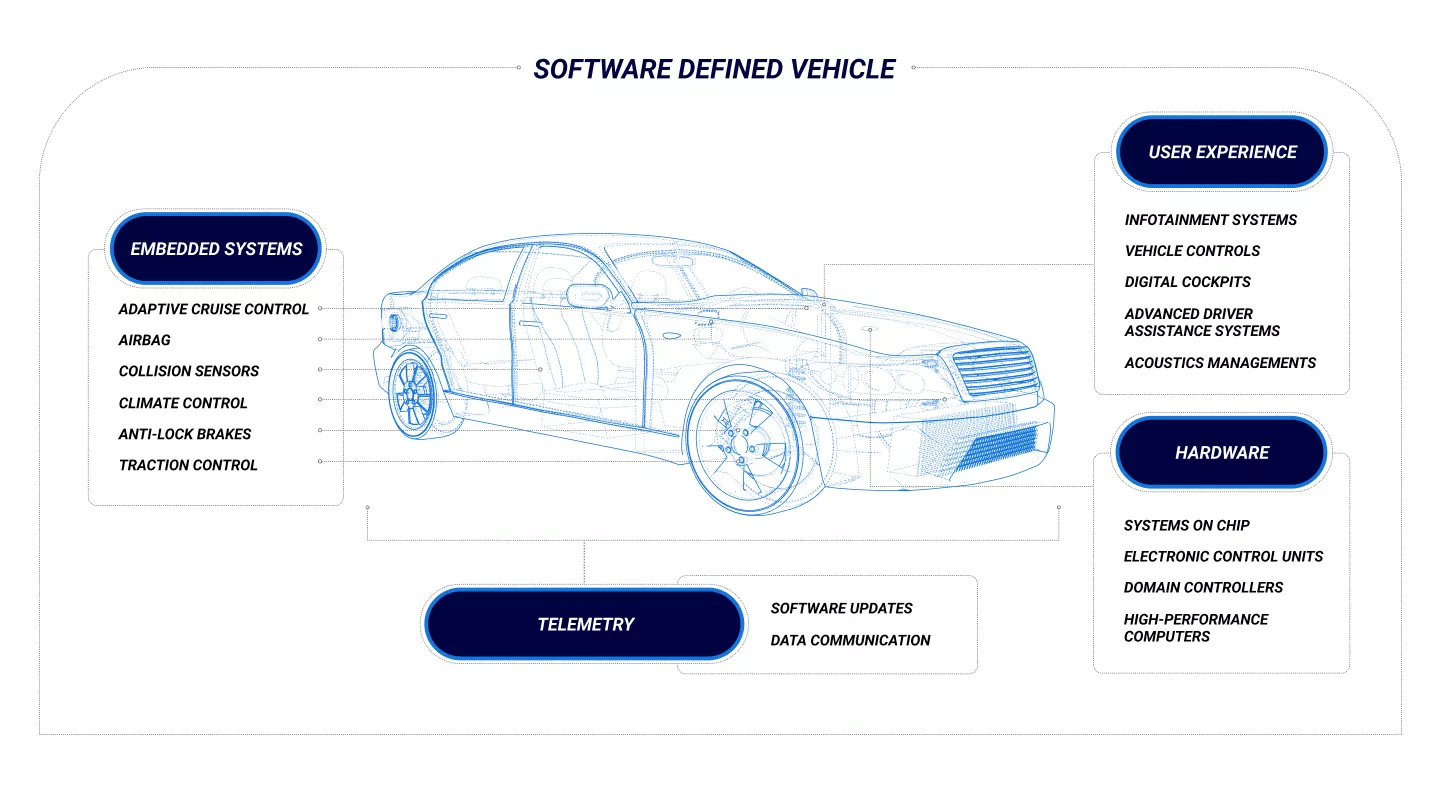
\includegraphics[scale=0.32]{Figures/SDV.png}
  	\caption{Software defined vehicles}
  	\label{fig:Software defined vehicles}
\end{figure}

At its core, an SDV relies on software systems to control and manage various aspects of the vehicle's operations. These software systems govern functions such as engine management, powertrain control, braking, steering, and infotainment systems. By utilizing software, SDVs can offer improved performance, increased safety, and enhanced user experiences.

One of the key features of SDVs is their ability to collect and analyze vast amounts of data from various sensors and sources within the vehicle. This data includes information from cameras, radars, LiDARs, GPS, and other sensors, which is processed and utilized for various purposes such as object detection, collision avoidance, adaptive cruise control, and autonomous driving capabilities.

SDVs also leverage connectivity technologies to interact with the external environment. They can communicate with other vehicles, infrastructure systems, and cloud-based services to exchange information, access real-time data, and enhance driving experiences. Connectivity enables features like vehicle-to-vehicle (V2V) and vehicle-to-infrastructure (V2I) communication, enabling cooperative driving, traffic optimization, and enhanced safety.

Furthermore, SDVs often incorporate advanced software update mechanisms, allowing manufacturers to remotely deploy software updates and enhancements to vehicles. Over-the-air (OTA) updates eliminate the need for physical visits to service centers, providing convenience, efficiency, and the ability to continuously improve and upgrade vehicle functionalities.

The concept of SDVs also extends beyond individual vehicles. It encompasses the integration of vehicles into larger smart mobility ecosystems, where vehicles can communicate and collaborate with each other, infrastructure systems, and mobility service providers. This integration facilitates intelligent transportation systems, shared mobility, and the potential for more efficient and sustainable transportation solutions.

Overall, SDVs represent the convergence of software, connectivity, and advanced technologies in the automotive industry. By leveraging software-defined capabilities, these vehicles offer enhanced performance, safety, connectivity, and intelligent features, paving the way for the future of mobility.

\section{Problem statement}
\subsection{Safety and Security}
One of the key challenges in the development of Software-Defined Vehicles (SDVs) is ensuring the safety and security of the software and communication systems. As SDVs rely heavily on software algorithms, connectivity, and data exchange, vulnerabilities and potential cyber threats pose significant risks. The project aims to address the challenge of designing robust security measures, implementing secure communication protocols, and developing reliable fail-safe mechanisms to ensure the safety of SDVs and protect against potential cyberattacks.

\subsection{Standardization and Interoperability}
With the rapid evolution of SDV technologies, the lack of standardization and interoperability among different components and systems is a significant challenge. SDVs involve complex software architectures, multiple sensors, communication networks, and control systems, making it crucial to establish common standards and protocols for seamless integration and interoperability. The project focuses on exploring and developing standardized frameworks, protocols, and interfaces that enable interoperability between various SDV components, facilitating collaboration and compatibility among different manufacturers and service providers.
\subsection{Ethical and Legal Implications}
As SDVs become more advanced and autonomous, ethical and legal considerations arise. The project addresses questions related to liability, responsibility, and decision-making in critical situations. It explores the ethical implications of autonomous decision-making algorithms, such as how SDVs prioritize safety, handle potential accidents, and navigate complex moral dilemmas. Additionally, the project delves into the legal frameworks and regulatory requirements necessary to govern the deployment and operation of SDVs, ensuring compliance with local and international laws.

\subsection{User Acceptance and Trust}
The successful adoption of SDVs relies on user acceptance and trust in the technology. The project examines factors influencing user perception, concerns, and attitudes towards SDVs, including issues such as privacy, data collection, and the reliability of autonomous systems. It aims to identify strategies to increase user acceptance, improve transparency, and build trust by addressing user concerns through effective communication, education, and user-centered design principles.

\subsection{Infrastructure Readiness}
The deployment of SDVs requires a supportive infrastructure that includes robust communication networks, intelligent transportation systems, and infrastructure-to-vehicle connectivity. The project investigates the readiness of existing infrastructure to accommodate SDVs and identifies the necessary upgrades and investments needed to enable seamless integration and communication. It explores challenges related to network coverage, latency, data transmission, and infrastructure compatibility to ensure the infrastructure can support the demands of SDVs effectively.

\chapter{TCU Architecture}
\section{Overview of the TCU Functionality}
The Telematics Control Unit (TCU) implemented in this project aims to transform conventional vehicles into software-defined vehicles with advanced features including Vehicle-to-Vehicle (V2V) and Vehicle-to-Cloud (V2C) communication capabilities. The TCU incorporates various functionalities to enhance vehicle connectivity, safety, customization, and communication with external entities.
The TCU acts as the central hub for managing the telematics and connectivity capabilities of the vehicle. It serves as the interface between the vehicle's internal systems and the external world, enabling communication, data transfer, and remote-control functionalities. By leveraging the power of the TCU, automakers can introduce a wide range of software-defined features and services, enhancing both the driving experience and the overall functionality of the vehicle. Here are more details on the TCU functions.

\section{Software defined vehicle overview (SDV)}
The Software Defined Vehicle (SDV) is a concept that involves the ability to upgrade and enhance a car's functionality throughout its lifetime by leveraging a centralized architecture and integrating new applications. This concept is seen as the next revolution in the automotive industry. Similar to how smartphones can receive software updates and new applications to enhance their capabilities, SDVs follows a similar principle but on a much more complex scale. The software-defined approach allows for flexibility and agility in the automotive industry. Instead of relying solely on hardware upgrades or replacing the entire vehicle, SDVs offer the possibility of enhancing and extending the vehicle's capabilities through software updates. 

\begin{figure}[!ht]
\centering
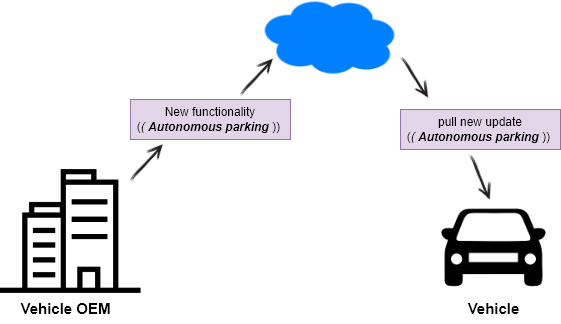
\includegraphics[scale=0.5]{Figures/1.png}
\caption[vehicle OTA Update]{vehicle OTA Update}
\label{fig:TCU}
\end{figure}

The adoption of Software Defined Vehicles empowers OEMs to continually enhance the capabilities of their vehicles by delivering new features through software updates over the air. This opens up opportunities for improved business models where end users can purchase additional features for their vehicles even after they have left the dealership.



\section{V2C Communication overview}
The TCU supports Vehicle-to-Cloud (V2C) communication. This functionality enables the vehicle to establish a connection with a cloud-based infrastructure, allowing bidirectional communication between the vehicle and the cloud. V2C communication opens up a wide range of possibilities, such as remote diagnostics, software updates, and personalized services for vehicle owners. It enables the vehicle to send data to the cloud for analysis and receive commands or information from the cloud, enhancing functionality, efficiency, and user experience.

\subsection{Integration with Cloud Backend overview}
The TCU integrates with a cloud backend, enabling V2C communication and providing a gateway for interactions with external systems. Through this integration, the vehicle can transmit and receive data to and from the cloud infrastructure securely. V2C communication enables various services, such as remote vehicle monitoring, data analytics, and personalized services, which can be delivered to the vehicle from the cloud. The TCU utilizes cloud connectivity for OTA updates, remote diagnostics, and other cloud-based services.

\section{V2V Communication overview}
The TCU enables Vehicle-to-Vehicle \cite{biswas2006vehicle} (V2V) communication, allowing vehicles to exchange critical information with each other. This functionality enhances road safety by facilitating the sharing of real-time data, such as location, speed, and potential hazards, among nearby vehicles. This information exchange enables the implementation of cooperative features like cooperative adaptive cruise control, where vehicles can maintain a safe distance and adjust their speed collectively, improving traffic flow and reducing accidents. V2V communication can also enhance safety by alerting drivers to potential hazards, such as sudden braking or approaching emergency vehicles. V2V communication helps drivers make informed decisions and mitigates potential accidents.

\begin{figure}[!ht]
\centering
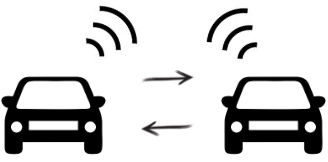
\includegraphics[scale=0.5]{Figures/V2V communication data exchange between vehicles.png}
\caption[V2V Communication overview]{V2V communication data exchange between vehicles}
\label{fig:V2V communication data exchange between vehicles}
\end{figure}
 


\section{Communication with External ECUs overview}
The TCU (Transmission Control Unit) seamlessly integrates with external Electronic Control Units (ECUs) by utilizing Ethernet communication as well as other embedded communication protocols such as SPI and UART. By employing Ethernet, the TCU ensures reliable and high-speed data exchange between itself and the external ECUs, facilitating smooth integration with diverse vehicle systems. This advanced communication protocol enhances the TCU's capability to connect and interact with various components, contributing to efficient and seamless vehicle operations.

\section{Industry Standards and Ecosystem Integration}
The TCU adheres to industry standards such as SOAFEE initiative. By following its standards, the TCU ensures seamless connectivity and integration within the vehicle ecosystem and with external entities. It promotes compatibility with other components, systems, and services, enabling efficient and standardized communication.

\section{TCU Layered Architecture}



The TCU software architecture based on the Linux operating system follows a layered approach, which allows for modularity, scalability, and ease of maintenance. Each layer focuses on specific functionalities and interacts with the layers above and below it.

The TCU layered software architecture is designed to provide robust and reliable connectivity and communication capabilities for vehicles. The architecture comprises several layers that work together to enable the functionality and communication of the system as visualized in figure \ref{fig:TCUs Layered architecture}.
\clearpage

\begin{figure}[h]
\centering
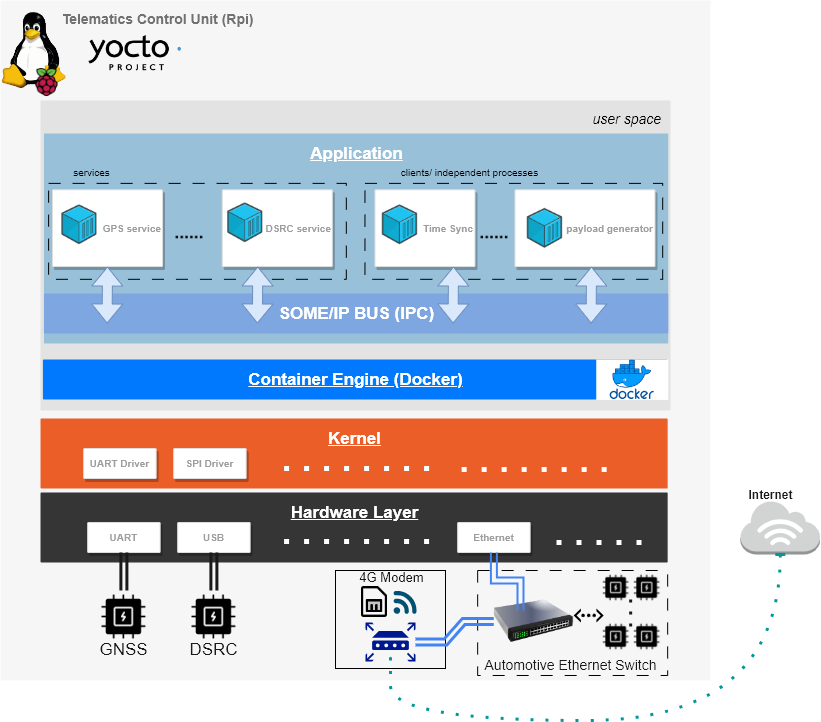
\includegraphics[scale=0.5]{Figures/TCUs Layered architecture.png}
\caption[TCUs Layered architecture]{TCUs Layered architecture}
\label{fig:TCUs Layered architecture}
\end{figure}

The TCU architecture includes an application layer where microservices communicate through IPC using SOME/IP protocol, Docker container runtime environment, the Linux Kernel, and the hardware layer. 
Let's explore the layers of the TCU software architecture in more details from bottom-up: 
\subsection{Hardware Layer}
The hardware layer represents the physical components and peripherals that constitute the TCU. This layer includes processors, memory, storage, network interfaces, and other hardware elements necessary for the TCU's operation.
The Hardware Layers provides:
    \begin{itemize}
      \item External devices communication: TCU establishes communication with external devices such as the GNSS receiver using the UART protocol for location information, and with the DSRC transceiver via USB 3.0 for V2V communication. 
      \item Connection with other ECUs: The connection between the TCU and other ECUs in the vehicle is facilitated through an ethernet switch where the TCU is connected to, which acts as a central hub for communication between the TCU and the various ECUs.
      \item Internet connectivity: The TCU is connected to the internet by utilizing an Ethernet interface, enabling internet access for tasks such as data exchange, accessing cloud services, and software updates.
    \end{itemize}
\subsection{Kernal Layer}
    At the Linux kernel level, the TCU interacts with the operating system's kernel, which is responsible for managing the hardware resources and providing an interface for software applications to access those resources. key aspects of the Linux kernel level in the TCU:
    \begin{itemize}
  \item Device Drivers – abstraction to low-level details: The Linux kernel utilizes device drivers to communicate with the hardware peripherals connected to the TCU. These device drivers serve as software interfaces that abstract the low-level details of the hardware, allowing the kernel to control and manage the hardware resources effectively as visualized in (figure4). Device drivers specific to the TCU's hardware components, such as processors, memory, storage, network interfaces, UART, SPI, and USB, are developed to enable seamless communication and control.
  \item Network Stack: The Linux kernel incorporates a robust network stack that handles network communication protocols and facilitates internet connectivity for the TCU. This network stack includes components like network drivers, protocols (TCP/IP, UDP, etc.), routing, and network address translation (NAT). It allows the TCU to establish network connections, transmit and receive data packets, and interact with external servers or cloud services over the internet.
\end{itemize}

  
\begin{figure}[h]
\centering
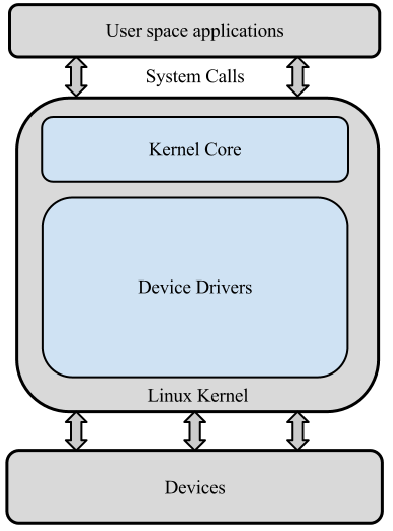
\includegraphics[scale=0.4]{Figures/LinuxKernel.png}
\caption[Kernel Layer]{User space application communicates with hardware through Linux Kernel APIs}
\label{fig:Kernel Layer}
\end{figure}
\clearpage

\subsection{Docker runtime environment Layer}
The Docker engine operates within the Linux user space layer, which we have identified as a separate layer responsible for running containerized applications. It is specifically designed to execute and manage containerized applications within the Application Layer.  The definition and customization of containerized applications behavior, is done using Docker Compose. It facilitates the configuration process using configuration YAML files. These files serve as a means to specify the desired settings and parameters for the Docker Compose. By employing YAML files, developers can easily define multiple services, their configurations, and interconnections in a structured manner. These configurations encompass various aspects such as environment variables, command-line arguments, volume mounts, and more. Here are the reasons why a container runtime environment is used.
\begin{itemize}
  \item Scalability and Resource Efficiency: Embedded systems often have limited resources in terms of processing power, memory, and storage. Containerization enables efficient utilization of these resources by isolating applications and their resource requirements. Each container can be optimized individually, allowing for better resource allocation and maximizing the performance of the overall system.
  
  \item Isolation and Security: Embedded systems run critical software components. Containerization provides strong isolation between different software components by ensuring that each application runs in its own containerized environment as visualized in (figure4). This isolation helps prevent conflicts and provides enhanced security by limiting the impact of vulnerabilities or misbehaving applications on the overall system.
  
  \item Portability and Compatibility: Containers are designed to be highly portable, allowing applications to be deployed consistently across different hardware platforms and operating systems.
  
  \item Over-the-Air Updates: Finally, one of the biggest advantages of using Containerization is that it simplifies the process of delivering over-the-air updates to vehicles. By using containers, manufacturers can package software updates into isolated units that can be securely deployed and activated on vehicles without disrupting the entire system.
\end{itemize}

\clearpage

\begin{figure}[h]
\centering
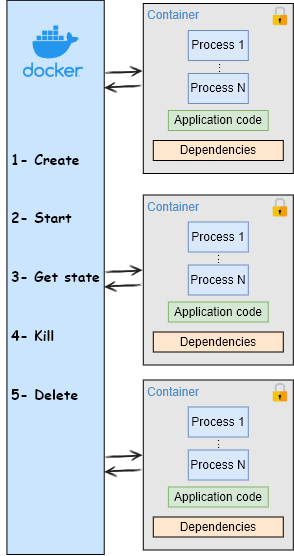
\includegraphics[scale=0.5]{Figures/5.png}
\caption[Docker runtime environment Layer]{Docker runtime environment Layer}
\label{fig:5}
\end{figure}

\subsection{Application Layer and VSOME/IP}
The application layer encompasses the telematics functionalities and services provided by the TCU. The application layer is responsible for hosting the containerized services that provide the primary functionality of the system. It includes modules for vehicle diagnostics, over-the-air updates, telematics services, and other specific applications. To enable seamless communication and data exchange between these services, an Inter-Process Communication (IPC) mechanism is employed.

\begin{itemize}
  \item Hosting containerized services: This layer is responsible for hosting the containerized services that provide the primary functionality of the TCU, creating a Service-Oriented Architecture (SOA).
  \item Inter-Process Communication (IPC) using VSOME/IP: The TCU employs an IPC mechanism for communication and data exchange between the containerized services within the application layer. The IPC is implemented through VSOME/IP, utilizing the standardized SOME/IP protocol for efficient and reliable communication between different services.
  \item Service-Oriented Architecture (SOA): VSOME/IP follows a service-oriented architecture approach, where software components or services communicate with each other through well-defined interfaces. It allows for the decoupling of components, promoting modularity and reusability. VSOME/IP provides a standardized means for components within the TCU to exchange data and control information, ensuring seamless interoperability.
  \item Publish/Subscribe Pattern: VSOME/IP supports the publish/subscribe pattern, where the containerized services can publish messages (events or data) to a specific topic, and interested subscribers can receive those messages.
\end{itemize}

\chapter{Hardware Components of the TCU}
\section{Raspberry Pi 4B SOC}
\subsection{What is the Raspberry Pi 4B?}
The Raspberry Pi 4 Model B is a popular single-board computer (SOC) developed by the Raspberry Pi Foundation. It is the fourth generation of the Raspberry Pi series and offers significant improvements over its predecessors.

The Raspberry Pi 4 offers powerful performance with its quad-core Cortex-A72 processor, multiple RAM options, and support for dual 4K displays, making it suitable for a wide range of projects that require robust computing power. The board's connectivity options, including USB 3.0 ports, Gigabit Ethernet, and wireless capabilities, further enhance its usability. With its affordable price point, accessibility, and extensive support available, the Raspberry Pi 4 stands out as a highly versatile and user-friendly SOC solution.
\begin{figure}[!ht]
\centering
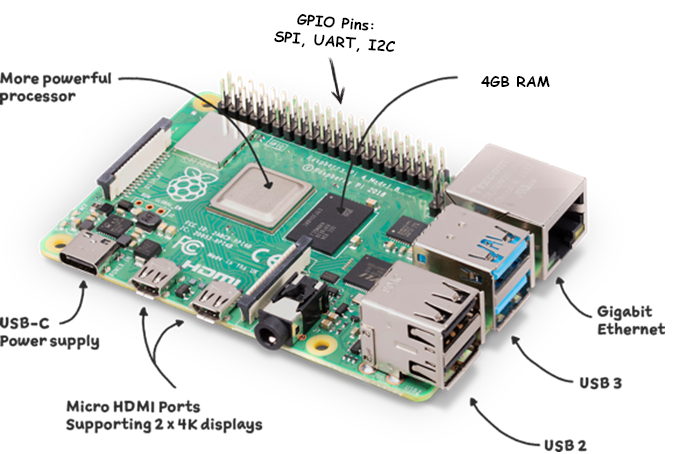
\includegraphics[scale=0.5]{Figures/6.png}
\caption[Raspberry-pi]{Raspberry-pi 4B layout}
\label{fig:6}
\end{figure}

\subsection{Raspberry Pi 4B Specifications}
Performance: The Raspberry Pi 4 is a powerful device, featuring a Broadcom BCM2711 quad-core Cortex-A72 processor running at 1.5GHz. This provides a substantial performance boost compared to previous models, making it suitable for a wide range of applications.

RAM Options: The Raspberry Pi 4 is equipped with 4GB of RAM, which allows for smoother multitasking and better performance when running over a hundred services on the TCU.

Connectivity: The Raspberry Pi 4 boasts improved connectivity options, including two USB 3.0 ports and two USB 2.0 ports. These ports enable faster data transfer speeds when connecting external devices. Additionally, it incorporates a Gigabit Ethernet port that offers high-speed internet connectivity.

Storage: The board features a microSD card slot for the operating system and storage. It also has two USB 3.0 ports and two USB 2.0 ports, allowing for external storage devices to be connected.

Operating Systems: The Raspberry Pi 4 supports a variety of operating systems, including the official Raspberry Pi OS (formerly known as Raspbian), as well as popular Linux distributions like Ubuntu, Fedora, and others. It can also run other specialized operating systems like RetroPie for gaming emulation. In our case, we build our own Linux OS using the Yocto Project.

GPIO Pins: Like previous Raspberry Pi models, the Raspberry Pi 4 has a 40-pin GPIO (General Purpose Input/Output) header, which allows for interfacing with external devices and expansion boards. This makes it suitable for electronics and prototyping projects.

Power: The Raspberry Pi 4 requires a USB-C power supply. It is recommended to use a power supply with a rating of 5V and at least 3A to ensure stable operation, which is provided to it through a 12V to 5V step-down buck converter.

\section{The DSRC Module}
DSRC (Dedicated Short-Range Communications) is a wireless communication technology designed specifically for automotive and transportation applications. It enables communication between vehicles (V2V) and between vehicles and infrastructure (V2I) to enhance safety, efficiency, and overall transportation system performance.

DSRC operates in the 5.9 GHz frequency band and utilizes IEEE 802.11p as the underlying communication standard. This frequency band is globally allocated for Intelligent Transportation Systems (ITS) and provides a dedicated spectrum for vehicle communication, ensuring reliable and low-latency communication in a short-range environment.

The primary goal of DSRC is to enable cooperative systems that can share important information among vehicles and infrastructure. This information includes vehicle position, speed, acceleration, braking status, and other relevant data that can be used to improve road safety and traffic efficiency. By providing real-time communication, DSRC allows vehicles to exchange data and coordinate actions to prevent accidents, reduce traffic congestion, and optimize traffic flow.

DSRC supports various applications and services to enhance road safety and transportation efficiency. These include:

\begin{itemize}
    \item Collision Avoidance: DSRC enables vehicles to exchange information about their speed, heading, and location, allowing them to detect potential collision risks and take preventive measures.
    \item Intersection Safety: DSRC allows vehicles and traffic infrastructure (e.g., traffic lights) to communicate, enhancing safety at intersections by providing warnings and coordinating traffic movements.
    \item Cooperative Adaptive Cruise Control (CACC): DSRC facilitates platooning, where a group of vehicles can travel in close proximity and maintain a constant speed through coordinated acceleration and braking. This can improve traffic flow and reduce fuel consumption.
    \item Emergency Vehicle Warning: DSRC enables emergency vehicles to transmit their position, direction, and status to surrounding vehicles, notifying drivers in advance and allowing them to make way efficiently.
    \item Road Weather Information: DSRC can deliver real-time weather and road condition information to vehicles, helping drivers adapt their driving behavior to changing conditions and improving overall safety.
    \item Infrastructure-to-Vehicle Communication (I2V): DSRC enables traffic infrastructure, such as road signs or traffic management systems, to communicate with vehicles, providing drivers with real-time information and warnings.
\end{itemize}

While DSRC has shown promise in enhancing road safety and transportation efficiency, it faces some challenges and competition from emerging technologies. One such technology is Cellular Vehicle-to-Everything (C-V2X), which utilizes cellular networks for communication. The ongoing debate between DSRC and C-V2X has led to uncertainty regarding the future of DSRC deployment.

However, DSRC modules are not readily available in Egypt due to their working frequency, making it difficult to procure them for our project. Additionally, due to regulatory restrictions, exporting DSRC modules from other countries was not feasible. Therefore, we needed to find an alternative solution that could provide similar functionality to DSRC.

To address this challenge, we opted to utilize ESP32/8266 microcontrollers as a replacement for DSRC modules. These microcontrollers support the ESP-NOW communication protocol, which allows direct communication between ESP32/8266 chips without the need for a centralized access point or router. By leveraging the ESP-NOW protocol, we were able to establish reliable and efficient communication between vehicles, enabling the exchange of vital information and mimicking the core functionality of DSRC.

\section{ESP32/8266 and ESP-NOW Protocol}
ESP-NOW \cite{ESP-NOW} is a communication protocol developed by Espressif Systems, the company behind the ESP8266 and ESP32 microcontroller platforms. It enables low-power, low-latency, and peer-to-peer communication between ESP8266 and ESP32 devices without the need for an existing Wi-Fi network.

ESP-NOW operates in the 2.4 GHz frequency band and uses a simple point-to-point or broadcast communication model. It is designed for scenarios where devices need to communicate directly with each other, such as sensor networks or home automation systems.

Some key features of ESP-NOW include:

\begin{itemize}
    \item Low Power: ESP-NOW is optimized for low power consumption, making it suitable for battery-powered applications.
    \item Low Latency: The protocol provides fast and efficient communication between devices with minimal latency.
    \item Peer-to-Peer Communication: ESP-NOW enables devices to communicate directly with each other without the need for a central access point or Wi-Fi network.
    \item Simple API: The API for implementing ESP-NOW is straightforward, making it relatively easy to integrate into projects.
    \item Secure Communication: ESP-NOW supports AES encryption, ensuring secure data transmission between devices.
\end{itemize}

ESP-NOW can be used in various applications, such as remote sensing, home automation, industrial monitoring, and wireless mesh networks. It allows ESP8266 and ESP32 devices to form a network and exchange data efficiently and reliably. This approach enabled us to overcome the unavailability of DSRC modules and regulatory limitations, allowing us to proceed with our project and achieve the desired communication capabilities in an unlicensed frequency band.

The ESP32/8266 leverages the ESP-NOW communication protocol to facilitate data exchange with nearby vehicles. It utilizes the ESP32's ESP-NOW communication protocol to send and receive data with all surrounding vehicles and sends the received data to the Encoder-Decoder on the same Raspberry Pi the ESP is connected to. It also receives data from the Encoder-Decoder on that same Raspberry Pi, which represents the data received from the available sensors of the vehicle, and broadcasts the data to surrounding vehicles. ESP-NOW is a lightweight protocol that allows direct communication between ESP32 chips without the need for a centralized access point or router.

\begin{figure}[!ht]
\centering
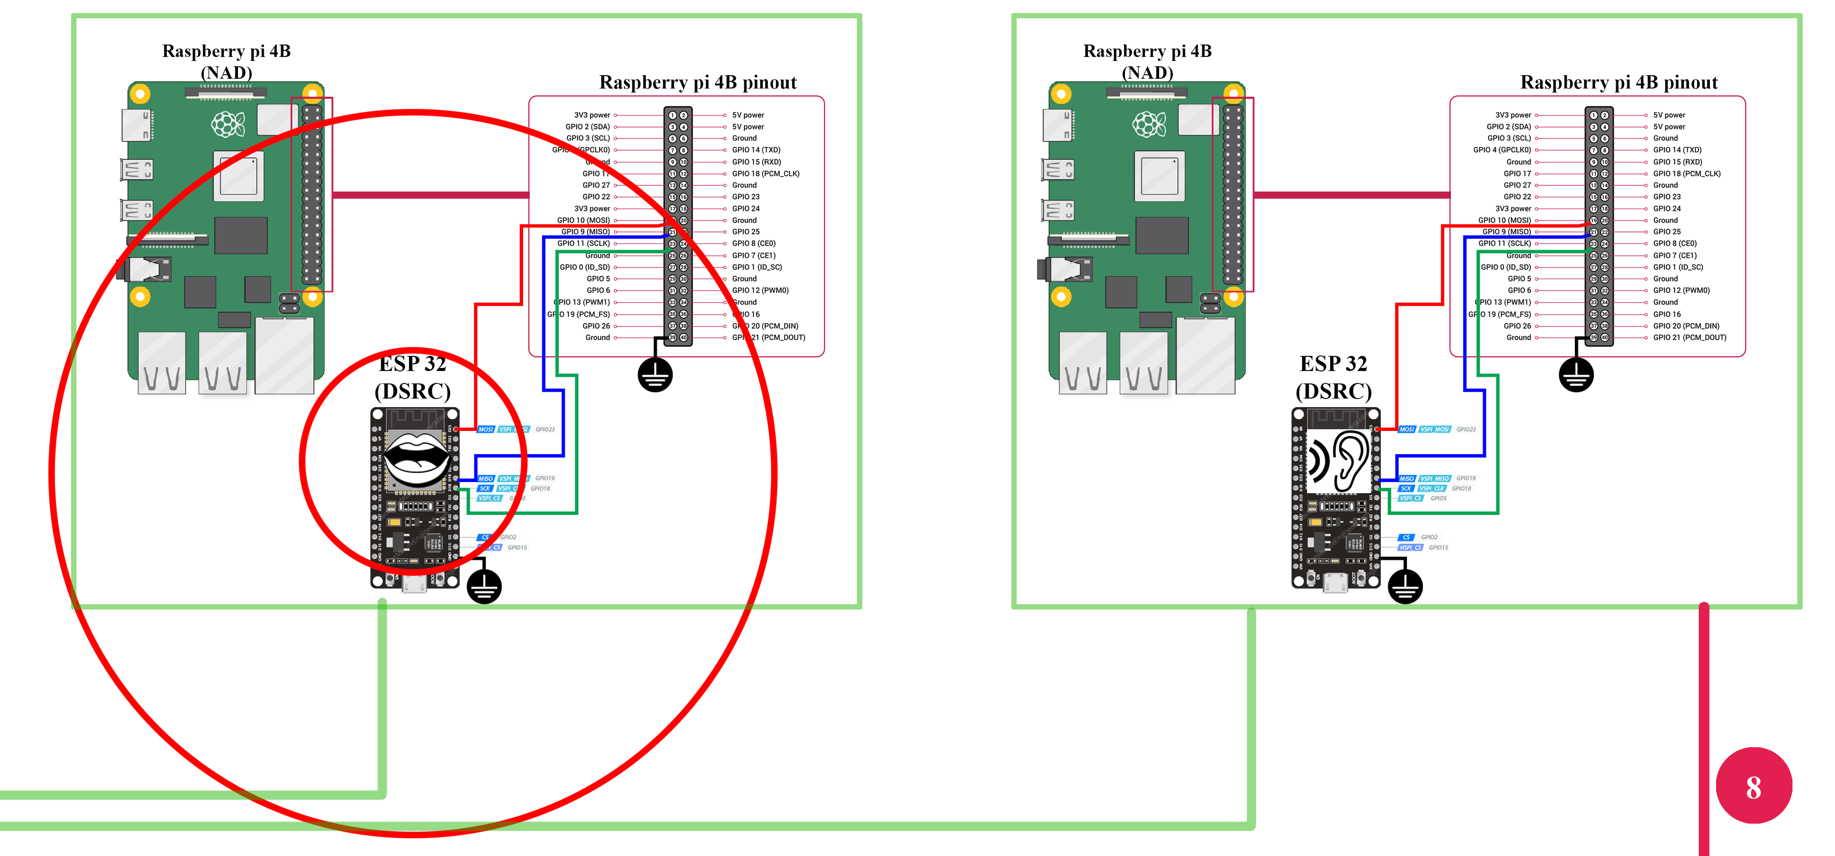
\includegraphics[scale=0.2]{Figures/7.png}
\caption[Sender/Receiver ESP Node Diagram]{Sender/Receiver ESP Node Diagram}
\label{fig:TCU}
\end{figure}

Upon initialization, the program sets up the ESP32 in station (STA) mode, disconnects from any previously connected Wi-Fi network, and initializes ESP-NOW. It also registers a receive callback function (receiveCallback()) and a send callback function (sentCallback()).
\begin{figure}[!ht]
\centering
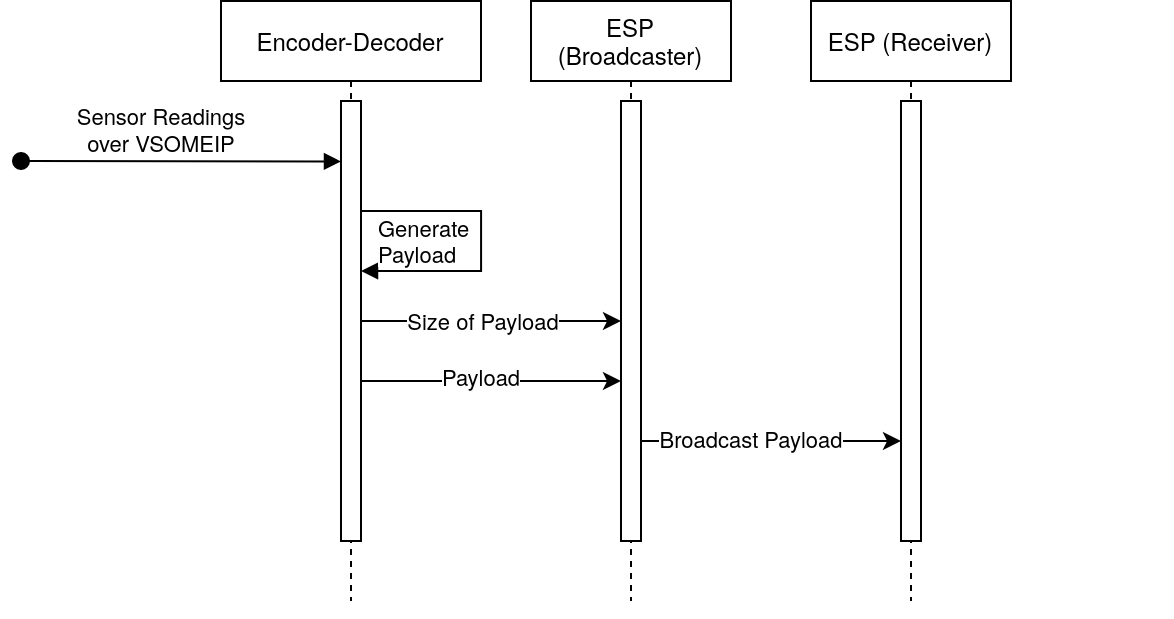
\includegraphics[scale=0.5]{Figures/8.png}
\caption[Data broadcasting UML Sequence diagram]{Data broadcasting UML Sequence diagram}
\label{fig:TCU}
\end{figure}

\begin{figure}[!ht]
\centering
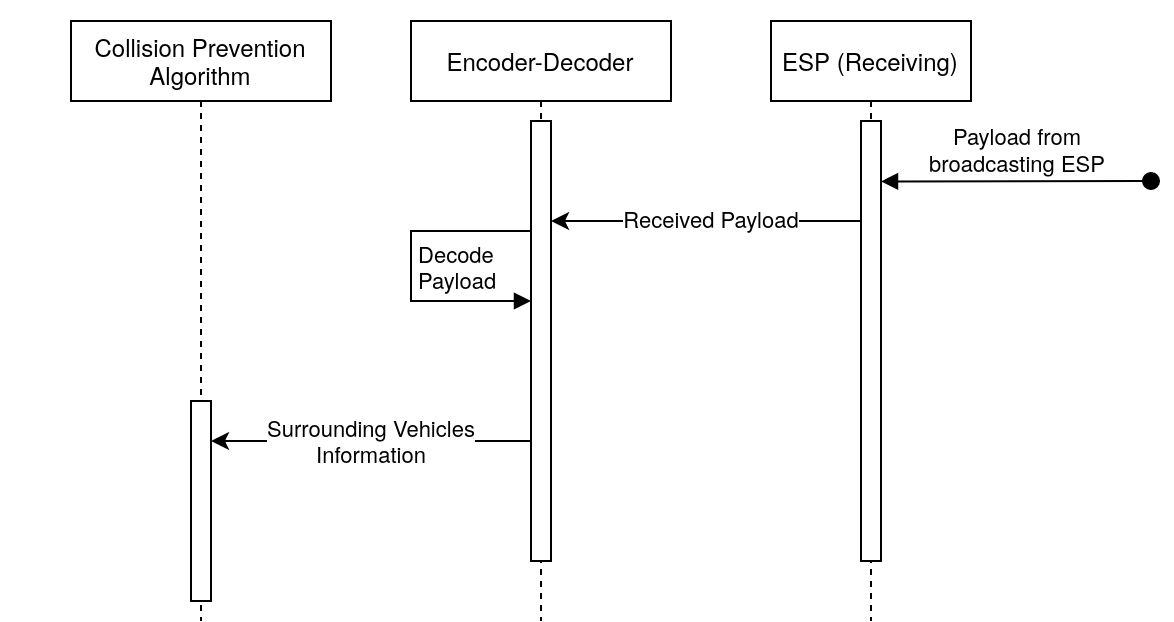
\includegraphics[scale=0.5]{Figures/9.png}
\caption[Data Reception UML Sequence diagram]{Data Reception UML Sequence diagram}
\label{fig:TCU}
\end{figure}
The receiveCallback() function is called whenever a valid packet is received via ESP-NOW as visualized in  (figure7). It extracts the MAC address and data from the received packet, formats the MAC address into a printable string with minimum format possible (0xFF0xFF0xFF0xFF0xFF0xFF), The program optimizes the data transmission by eliminating unnecessary characters, allowing the data to be sent in the smallest possible size without any superfluous additions. And prints debug information to the serial port when needed. The received payload is then concatenated with the MAC address of the sender and with any identification numbers available and then send over UART from the ESP to the Encoder-Decoder software. 
The broadcast() function is responsible for broadcasting a message to all devices in range. It prepares the broadcast address (0xFF:0xFF:0xFF:0xFF:0xFF:0xFF) which represents all surrounding vehicles of whatever mac address, and then sends the message to all surrounding vehicles.
Within the main loop of the ESP program, the program awaits incoming data on the serial port from the Encoder-Decoder which represents the data of the vehicle itself. It begins by reading a byte that represents the length of the data, followed by reading the remaining bytes into a buffer array. However, there is a possibility of the reading process being interrupted by a read timeout, which can result in the buffer being split and receiving incomplete data. This incomplete data can lead to inaccurate information processing by the receiver. Although adjusting the baud rate between the ESP and the Encoder-Decoder on the raspberry pi, still in some cases this issue persists.
To overcome this issue, the Encoder-Decoder program takes the approach of transmitting the size of each payload before sending the actual payload to the ESP (the receiver). This ensures that the ESP is prepared to receive a specific number of bytes. In the event that the ESP does not receive the expected number of bytes, it enters a loop and continues reading from the Encoder-Decoder program into the buffer. By doing so, the ESP can receive the complete data and avoid processing false information caused by incomplete transmissions.
After that, the payload is sent as a broadcast message using ESP-NOW protocol.
\begin{figure}[!ht]
\centering
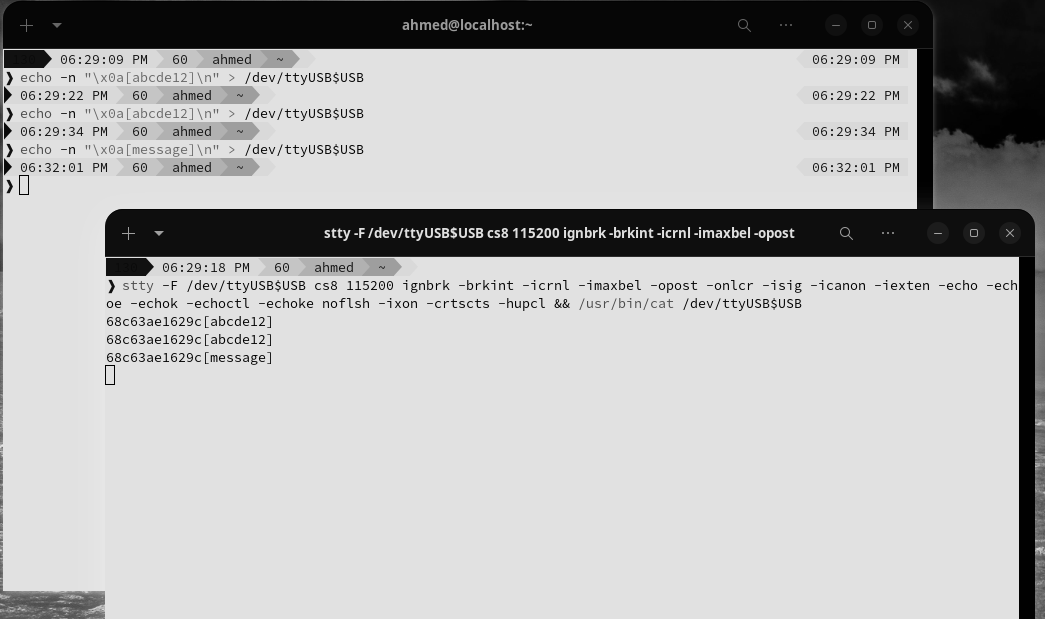
\includegraphics[scale=0.3]{Figures/10.png}
\caption[DSRC working example]{DSRC working example}
\label{fig:TCU}
\end{figure}
Overall, this code sets up the ESP32 as an ESP-NOW broadcaster and receiver. It receives data from the serial port from Encoder-Decoder and broadcasts it to other devices using ESP-NOW. Each ESP is also a receiver, whichever sends a message all surrounding ESPs receive it.

\section{U-Blox M8N GNSS}
\subsection{What is the U-blox M8N GNSS module}
The UBlox M8N GNSS (Global Navigation Satellite System) is a high-performance positioning module. The M8N module is specifically designed to provide precise and reliable satellite positioning data for a wide range of applications, including navigation, timing, and tracking systems. The u-blox M8N module supports multiple satellite positioning systems, including GPS (Global Positioning System), GLONASS (Global Navigation Satellite System), Galileo, BeiDou, and QZSS (Quasi-Zenith Satellite System). This multi-GNSS compatibility ensures better accuracy, reliability, and availability of satellite signals, especially in challenging environments.


\begin{figure}[!ht]
\centering
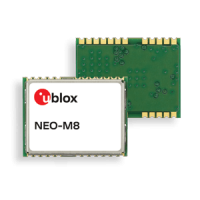
\includegraphics[scale=0.5]{Figures/11.png}
\caption[U-blox M8N GNSS]{U-blox M8N GNSS}
\label{fig:TCU}
\end{figure}

\subsection{U-blox M8N Specifications}
The U-Blox M8N GNSS module offers several features that make it suitable for vehicle Telematics Control Units. Some of its key features and specifications include:

\begin{itemize}
  \item Small Form Factor: The M8N module is available in a compact surface-mount package, making it easy to integrate into a wide range of devices and systems. Its small size and lightweight design (as visualized in Figure 6) enable seamless integration.
  \item High Accuracy: The u-Blox M8N GNSS module leverages advanced positioning algorithms and precise timing techniques to achieve high accuracy positioning. It provides centimeter-level accuracy for real-time positioning, making it ideal for applications requiring precise vehicle tracking or navigation.
  \item External Antenna Port: The u-blox M8N GNSS module offers the flexibility to add an external antenna (see Figure 8 and Figure 7), allowing users to enhance the positioning performance and overcome signal reception challenges. The module provides an interface for connecting an external active or passive antenna, enabling better signal reception in environments with limited sky visibility or high levels of interference.
\end{itemize}

\begin{figure}[!ht]
\centering
\begin{minipage}{0.45\textwidth}
  \centering
  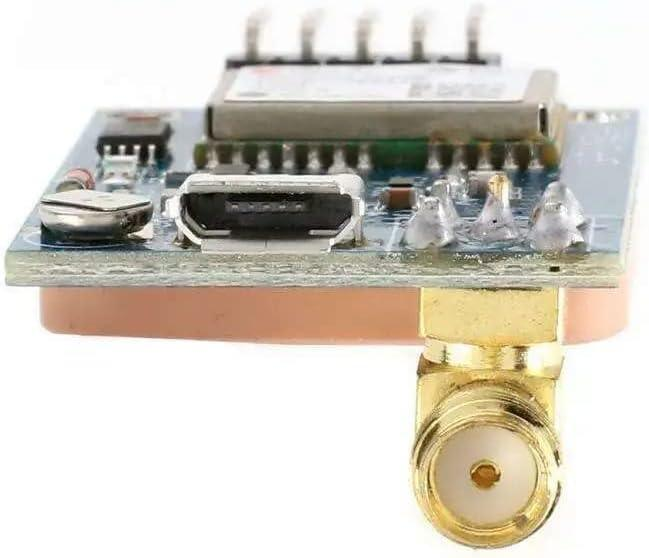
\includegraphics[width=\linewidth]{Figures/Ha.png}
  \caption[u-blox M8N module with external antenna port]{u-blox M8N module with external antenna port}
  \label{fig:M8N specifications}
\end{minipage}\hfill
\begin{minipage}{0.45\textwidth}
  \centering
  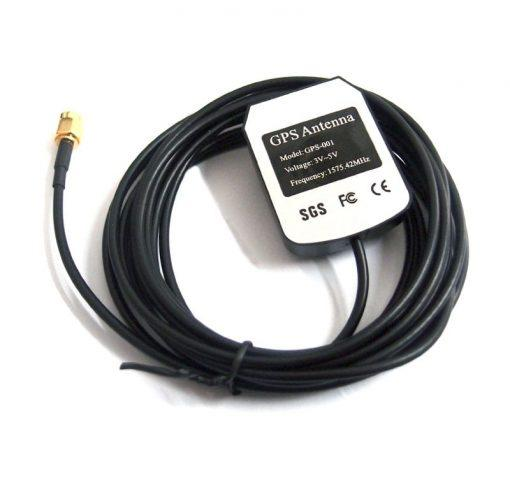
\includegraphics[width=\linewidth]{Figures/13.png}
  \caption[External GPS antenna]{External GPS antenna}
  \label{fig:External GPS antenna}
\end{minipage}
\end{figure}

Fast Time to First Fix (TTFF): The module has a fast Time to First Fix, which means it can acquire satellite signals quickly and determine the vehicle's position rapidly after power-up or signal loss. This feature ensures that the TCU can provide accurate positioning data without significant delays.
GNSS Support: The module supports multiple satellite systems, including GPS (Global Positioning System), GLONASS (Global Navigation Satellite System), Galileo, and BeiDou. This multi-constellation support enhances positioning accuracy and availability, even in challenging environments.
Dead Reckoning (DR) Support: The u-blox M8N GNSS module supports Dead Reckoning technology, which allows the TCU to estimate the vehicle's position based on its last known position, speed, and heading information. This feature is particularly useful in urban canyons or environments with limited satellite visibility, ensuring continuous positioning even when satellite signals are obstructed.
Power Efficiency: The module is designed to be power-efficient, consuming minimal power during operation. This characteristic is essential for telematics applications, as it helps optimize power consumption.
Communication Interfaces: The u-blox M8N GNSS module offers various communication interfaces, including UART (Universal Asynchronous Receiver-Transmitter), USB (Universal Serial Bus), and I2C (Inter-Integrated Circuit). These interfaces enable seamless integration with the TCU's communication architecture. In our TCU the u-blox module communicate with the Raspberry pi (SOC) through UART communication protocol.

Fast Time to First Fix (TTFF): The module has a fast Time to First Fix, which means it can acquire satellite signals quickly and determine the vehicle's position rapidly after power-up or signal loss. This feature ensures that the TCU can provide accurate positioning data without significant delays.
GNSS Support: The module supports multiple satellite systems, including GPS (Global Positioning System), GLONASS (Global Navigation Satellite System), Galileo, and BeiDou. This multi-constellation support enhances positioning accuracy and availability, even in challenging environments.
Dead Reckoning (DR) Support: The u-blox M8N GNSS module supports Dead Reckoning technology, which allows the TCU to estimate the vehicle's position based on its last known position, speed, and heading information. This feature is particularly useful in urban canyons or environments with limited satellite visibility, ensuring continuous positioning even when satellite signals are obstructed.
Power Efficiency: The module is designed to be power-efficient, consuming minimal power during operation. This characteristic is essential for telematics applications, as it helps optimize power consumption.
Communication Interfaces: The u-blox M8N GNSS module offers various communication interfaces, including UART (Universal Asynchronous Receiver-Transmitter), USB (Universal Serial Bus), and I2C (Inter-Integrated Circuit). These interfaces enable seamless integration with the TCU's communication architecture. In our TCU the u-blox module communicate with the Raspberry pi (SOC) through UART communication protocol.

\chapter{Linux OS and Kernel Layer}
\section{Building Custom Image Using Yocto Project}
\subsection{Introduction}
The Yocto Project is an open-source collaboration project that provides a flexible and customizable framework for building embedded Linux systems. Its primary purpose is to simplify the process of creating Linux distributions tailored for specific embedded devices or platforms. By leveraging the Yocto Project, developers can efficiently build and maintain custom Linux-based solutions, enabling them to focus on developing their applications rather than dealing with the intricacies of the underlying software stack.

The Yocto Project offers a set of tools, documentation, and a standardized methodology for building embedded Linux systems. It utilizes the concept of "layers," which are modular components that define different aspects of the build, such as hardware support, Linux kernel configuration, software packages, and system configurations. These layers can be customized and extended to meet the specific requirements of the target device or platform.

The Yocto Project's core tool, called "BitBake," is a build engine that orchestrates the build process. It manages the tasks of fetching source code, configuring the build environment, compiling packages, and generating the final system image. BitBake relies on metadata files called "recipes" to define the build instructions for each component in the system. These recipes specify the source URLs, compilation flags, dependencies, and other necessary information for building each package.

One of the key advantages of the Yocto Project is its ability to provide reproducible builds. This means that the build process can be precisely replicated across different environments, ensuring consistent and reliable results. The Yocto Project achieves this by utilizing "poky," a reference distribution that serves as a baseline for creating custom distributions. Developers can customize poky and add their own layers and packages to create a tailored Linux distribution for their specific needs.

Furthermore, the Yocto Project embraces the open-source philosophy, allowing developers to leverage a vast ecosystem of existing software components and tools. It provides a large collection of pre-built software packages, known as the "OpenEmbedded Core," which can be easily integrated into the build. This reduces the effort required to include popular libraries, frameworks, and applications in the final system image.

\subsection{Why custom OS?}
Customizing the operating system (OS) in embedded Linux is of paramount importance due to several reasons. Embedded systems are designed for specific tasks and have unique requirements that differ from general-purpose computing devices. By customizing the OS, we can optimize the system's performance, reduce resource usage, enhance security, and tailor the functionality to meet the specific needs of the embedded application.

One of the primary reasons for customizing the OS is to optimize performance. Embedded systems often have limited resources such as processing power, memory, and storage. By customizing the OS, unnecessary components, services, and functionalities can be removed or disabled, thereby reducing resource consumption and improving overall system performance. This optimization is crucial in embedded systems where efficiency is crucial.

Moreover, customization allows us to tailor the functionality of the OS to the specific requirements of the embedded application. Each application has its unique set of requirements, interfaces, and protocols. By customizing the OS, we can add or modify drivers, protocols, and interfaces to ensure seamless integration with the embedded hardware and other software components, leading to improved compatibility and functionality.

Customizing the OS also offers the advantage of reducing the system's footprint. Embedded systems often operate on constrained hardware, where every byte of storage matters. By eliminating unnecessary components and stripping down the OS to its essential elements, we can significantly reduce the system's size, leaving more storage space for the actual application and data.

Furthermore, customization enables us to optimize power consumption, a critical factor in many embedded systems. By fine-tuning the OS, unnecessary background processes and power-hungry features can be disabled or optimized, extending the battery life in portable devices or reducing power consumption in energy-conscious applications.

\subsection{Advantages of the Yocto Project}
\begin{itemize}
    \item Flexibility and Customization: The Yocto Project provides a highly flexible and customizable build system. It uses layers and recipes, allowing developers to easily add, modify, or remove components to create custom Linux distributions tailored to their specific requirements. The modular nature of the Yocto Project enables easy integration of additional software packages, configuration options, and hardware support.
    \item Wide Range of Supported Hardware: The Yocto Project supports a broad range of hardware architectures, including x86, ARM, MIPS, PowerPC, and more. It provides a unified framework that can be used across multiple hardware platforms, making it suitable for diverse embedded systems.
    \item Large Ecosystem and Community: The Yocto Project has a vibrant and active community of developers, contributors, and users. It benefits from a wide range of available documentation, tutorials, and resources, making it easier to get started and find solutions to common challenges. The community-driven nature of the Yocto Project ensures continuous improvement, bug fixes, and feature enhancements.
    \item Layered Architecture: The Yocto Project's layered architecture allows for better code reuse and modularity. Developers can leverage existing layers and recipes from the Yocto Project's extensive layer index, which provides a wealth of pre-configured and tested components. This layer-based approach simplifies the integration of software packages, device drivers, and board-specific configurations, speeding up the development process.
    \item Extensive Tooling and Automation: The Yocto Project offers a rich set of tools and utilities that automate the build process and facilitate system configuration. BitBake, the core build engine, provides sophisticated dependency management, parallel build capabilities, and incremental build support. Additionally, tools like the Poky Toolchain enable easy cross-compilation, making it simpler to develop and deploy software for embedded systems.
    \item Long-Term Support: The Yocto Project offers long-term support (LTS) releases, which ensure stability and reliability for production environments. LTS releases receive security updates, bug fixes, and maintenance for an extended period, providing a robust foundation for embedded systems with long product lifecycles.
    \item Industry Adoption and Standards Compliance: The Yocto Project is widely adopted by various industries and companies, including semiconductor manufacturers, embedded system vendors, and automotive companies. It adheres to industry standards and best practices, making it easier to integrate with existing tools, workflows, and development processes.
\end{itemize}


\subsubsection{Yocto Project vs Buildroot}
While Buildroot is a lightweight and straightforward alternative, we preferred to choose the Yocto Project for our project due to its flexibility, scalability, extensive ecosystem, and robust tooling. These factors make it a preferred choice for complex and customized embedded Linux distributions, aligning with our project's specific requirements and objectives.

\textbf{Flexibility:} The Yocto Project provides a highly flexible build system with layers and recipes, allowing us to customize and tailor the Linux distribution to our specific needs. We can easily add, modify, or remove components, configure hardware support, and define system configurations.

\textbf{Scalability:} The Yocto Project is designed to support a broad range of hardware architectures, making it suitable for our diverse embedded systems. It offers a unified framework that can be used across multiple platforms, ensuring scalability and adaptability as our project evolves.

\textbf{Extensive Ecosystem:} The Yocto Project benefits from a large ecosystem of pre-built software packages known as the OpenEmbedded Core. This extensive collection of components can be easily integrated into our build, reducing the effort required to include popular libraries, frameworks, and applications in the final system image.

\textbf{Robust Tooling:} The Yocto Project provides a rich set of tools and utilities, such as the core build engine BitBake and the Poky Toolchain. These tools automate the build process, manage dependencies, and enable easy cross-compilation. The sophisticated tooling ensures efficient development and deployment of software for our embedded systems.

While Buildroot may offer simplicity and a lightweight approach, it lacks the same level of flexibility, scalability, and extensive ecosystem as the Yocto Project. Buildroot may be more suitable for simple and straightforward projects with minimal customization requirements. However, considering our project's complexity and need for customization, the Yocto Project is better suited to meet our specific requirements and objectives.

\textbf{Conclusion:} With its flexibility, scalability, extensive ecosystem, and robust tooling, the Yocto Project provides the ideal solution for our project's embedded Linux distribution needs. We can leverage its features and benefits to efficiently build and maintain customized distributions that align with our project's goals.
\begin{figure}[!ht]
\centering

\includegraphics[scale=0.4]{Figures/16.png}
\caption[SOAFEE Architecture]{SOAFEE Architecture}
\label{fig:TCU}
\end{figure}

\section{Yocto Project Build Process}
\subsection{Setting Up The Yocto Environment}
To ensure a seamless integration of the Yocto Project into our Raspberry Pi-based project, the first step is obtaining the appropriate Board Support Package (BSP). In our case, we acquire the \texttt{meta-raspberrypi} BSP, specifically designed for Raspberry Pi boards. This BSP provides the necessary components, configurations, and drivers tailored to our target hardware.

Additionally, we need to consider the layer dependencies associated with the \texttt{meta-raspberrypi} BSP. This layer has a dependency on the \texttt{poky} layer, which serves as the foundation of the Yocto Project. The \texttt{poky} layer provides essential components, recipes, and tools required for building embedded Linux distributions. By leveraging the \texttt{poky} layer, we gain access to a comprehensive set of features and capabilities for our customized system.

In order to successfully install Yocto and achieve our desired functionality, we must also include the \texttt{meta-virtualization} layer and its associated layer dependencies. The \texttt{meta-virtualization} layer extends the capabilities of our Yocto Project-based system to support virtualization technologies. This layer allows us to incorporate virtual machines or containers within our embedded system, enabling efficient isolation and scalability for running applications and services.

The \texttt{meta-virtualization} layer itself depends on the \texttt{openembedded-core} layer, which is a core component of the Yocto Project. The \texttt{openembedded-core} layer provides foundational elements, including toolchains, libraries, and basic system configurations, necessary for building embedded Linux distributions. By incorporating the \texttt{openembedded-core} layer, we ensure the availability of fundamental components required for our Yocto Project implementation.

Moreover, the \texttt{meta-virtualization} layer relies on several other layers, such as \texttt{meta-oe}, \texttt{meta-networking}, \texttt{meta-filesystems}, and \texttt{meta-python}, which can be found within the \texttt{meta-openembedded} layer collection. Each of these layers brings additional functionality and features to our Yocto Project-based system. \texttt{Meta-oe} provides a range of additional packages and recipes, expanding the software options available to us. \texttt{Meta-networking} focuses on networking-related components and configurations, enabling us to integrate networking capabilities seamlessly. \texttt{Meta-filesystems} offers support for various file systems, accommodating different storage requirements. Lastly, \texttt{Meta-python} enhances our system's capabilities by providing Python-related packages and tools.

To align the Yocto Project with the specific needs of our project, we must modify the distribution configuration. This involves adding support for virtualization within the distribution, enabling us to leverage virtualization technologies effectively. By configuring the appropriate components, packages, and settings, we ensure that our embedded system can create and manage virtual machines or containers, facilitating the isolation and efficient utilization of system resources.

Furthermore, we choose to incorporate \texttt{systemd} as the init system within our Yocto Project-based distribution. \texttt{Systemd} offers advanced features for managing system services, dependencies, and boot processes. By integrating \texttt{systemd}, we benefit from its capabilities, such as parallel service startup, centralized logging, and reliable service management. This modification enhances the overall performance and maintainability of our embedded Linux system.

\subsection{Building core Image Minimal}
In our project, amidst the multitude of base image options provided by the Yocto Project, we have made a deliberate choice to leverage the \texttt{core-image-minimal} as the foundational base image. This particular image selection stems from careful consideration of our project requirements and goals, as well as the inherent advantages and benefits it offers.

The primary driving factor behind selecting the \texttt{core-image-minimal} is its inherent lightweight nature. As an intentionally minimalistic image, it contains only the bare essentials necessary for a functional embedded Linux system. By stripping away extraneous features, applications, and packages that are not crucial to our specific project requirements, we can achieve a lean and streamlined system that optimizes resource utilization and delivers efficient performance on our designated hardware platform---the Raspberry Pi board.

Furthermore, the \texttt{core-image-minimal} image serves as a solid foundation that allows a device to boot and establish a stable operating environment. Its compact size and stripped-down nature contribute to a faster boot time, enabling rapid system startup and responsiveness, which are particularly beneficial in resource-constrained embedded systems.

Additionally, the minimalist nature of the \texttt{core-image-minimal} image provides us with a high degree of flexibility and customization options. With a clean slate to begin with, we have the freedom to selectively add and integrate only the necessary software components and packages specific to our project requirements. This tailored approach empowers us to fine-tune the system to meet our exact needs without the burden of unnecessary bloat or complexity, resulting in a more efficient and focused embedded Linux distribution.

Moreover, the \texttt{core-image-minimal} image serves as a solid foundation for future expansion and customization. As our project evolves and additional features or functionalities are required, we can easily build upon this base image, adding specific layers, components, and configurations to meet the evolving demands of our application. The modular and extensible nature of the Yocto Project enables seamless integration of additional layers and packages, facilitating ongoing development and growth without the need for a complete system overhaul.

\subsection{Building Custom Layer}
In order to tailor the Yocto Project to our specific project requirements, we have taken the initiative to create and integrate a \texttt{meta-custom} layer. This \texttt{meta-custom} layer serves as a dedicated space where we can define and configure custom recipes that align with our project's unique needs and objectives.
Within the \texttt{meta-custom} layer, we have crafted recipes that facilitate the addition of users and the installation of packages that are crucial to the successful implementation of our project. By including these recipes, we ensure that the resulting embedded Linux distribution encompasses all the necessary components and functionalities required for our application.
To enable remote access and administration of our TCU (Raspberry Pi), we have incorporated the \texttt{openssh} package into our custom layer. This package allows us to establish secure SSH connections, granting us the ability to remotely manage and interact with the TCU. This remote access capability simplifies system administration tasks, facilitates troubleshooting, and enhances overall operational efficiency.
Given the nature of our application and the need for containerization, we have included the \texttt{docker} package in our custom layer. Docker provides us with a powerful and flexible containerization platform, allowing us to encapsulate our application and its dependencies within isolated containers. This approach offers numerous benefits, including portability, scalability, and simplified deployment across different environments.
To facilitate seamless file editing and configuration management, we have integrated the \texttt{nano} package into our custom layer. \texttt{Nano} is a user-friendly text editor that enables us to modify and customize various configuration files, scripts, and other textual resources. Its intuitive interface and feature set make it a convenient tool for developers and system administrators alike.
Furthermore, we have added the \texttt{git} package to our custom layer, which enables us to leverage the power of version control for our project's source code. \texttt{Git} provides a distributed and efficient version control system, allowing multiple team members to collaborate, track changes, and manage code repositories effectively. This inclusion ensures streamlined collaboration and enables us to maintain a well-organized and manageable codebase throughout the project's lifecycle.

With the completion of our \texttt{meta-custom} layer, encompassing the necessary recipes and package installations, we have initiated the Yocto Project build process. This process incorporates our customizations seamlessly, ensuring that the resulting embedded Linux distribution reflects our specific project requirements and delivers a tailored and optimized solution.

\section{Conclusion}
In conclusion, the Yocto Project build described incorporates several features and modifications to the bare \texttt{core-image-minimal}, expanding its capabilities and flexibility. The additions of OpenSSH, Nano, Git, and Docker bring secure remote access, convenient text editing, version control, and containerization to the embedded system. Furthermore, the implementation of systemd as the init system enhances service management, startup processes, and logging capabilities. These customizations not only enhance the functionality and performance of the system but also cater to specific requirements, streamlining development and deployment workflows.

Moreover, choosing Yocto Project over Buildroot offers several advantages. Yocto provides a comprehensive and extensible framework that enables developers to create highly customized and optimized embedded Linux systems. Its layer-based architecture and extensive package management system allow for easy integration of additional software components and customizations. The robust community support and extensive documentation of Yocto Project provide resources and knowledge sharing, aiding developers in their projects.

Additionally, Yocto's focus on reproducibility and its ability to generate complete and consistent builds ensure reliability and maintainability throughout the development process. The use of standardized metadata and recipes in Yocto simplifies the management of dependencies and updates, facilitating long-term support and ease of maintenance.

Overall, the Yocto Project offers a powerful and flexible platform for building embedded Linux systems, allowing for customization, scalability, and reproducibility, while benefiting from an active community and extensive documentation. These advantages make Yocto Project a compelling choice for developers seeking to create embedded systems tailored to their specific requirements.


\chapter{Containers run time Environment}
\section{Introduction}
Container runtime environment refers to a lightweight and isolated execution environment that allows for the deployment and execution of applications in a secure and efficient manner. This technology has gained popularity in the embedded systems domain due to its numerous benefits and use cases.

Containerization in embedded systems involves encapsulating applications and their dependencies within self-contained units called containers. These containers provide an isolated runtime environment that encapsulates the application, its libraries, and dependencies, ensuring consistent behavior regardless of the underlying hardware or operating system. This isolation helps to prevent conflicts between applications and provides a predictable execution environment, enhancing system stability and security.

Moreover, containerization simplifies the deployment and management of applications in embedded systems. Containers can be created, replicated, and distributed easily, streamlining the deployment process and allowing for rapid application updates and rollbacks.

Security is another key aspect of using container runtime environments in embedded systems. Containers provide isolation between applications and the underlying system, limiting the potential impact of a compromised application. Each container operates within its own runtime environment, with restricted access to system resources, enhancing overall system security and robustness.

Furthermore, the portability of containerized applications is advantageous in embedded systems. Applications can be developed and tested on a development machine, packaged as a container, and then deployed onto various embedded devices with consistent behavior. This simplifies the software development life cycle and enables faster time-to-market for embedded system applications.

\section{Containers vs Virtual Machines (VMs)}

In embedded systems, both containers and virtual machines (VMs) offer isolation and encapsulation of applications, but they have different approaches and characteristics.

Containers are generally more resource-efficient than VMs. They share the host system's operating system kernel, resulting in reduced overhead and efficient resource utilization. In contrast, VMs require a separate guest operating system for each instance, leading to higher resource consumption.

Containers provide better performance compared to VMs. They have lower startup times, faster application deployment, and less virtualization overhead. This makes them well-suited for real-time and latency-sensitive applications in embedded systems.

Both containers and VMs offer isolation, but at different levels. Containers achieve isolation by leveraging the host system's kernel and namespace separation mechanisms, ensuring application separation without the need for full operating system virtualization. VMs, on the other hand, provide complete isolation by running a separate operating system instance in each virtual machine as visualized in figure \ref{fig:container_vs_vm}.


\begin{figure}[h]
\centering
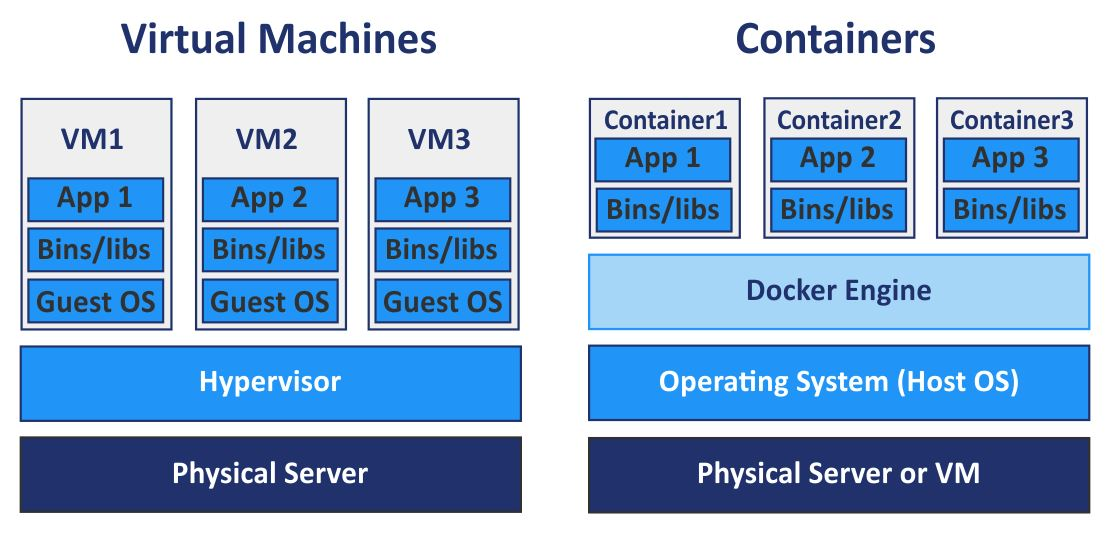
\includegraphics[scale=0.5]{Figures/containervsVM.JPG}
\caption[containers and VMs layered architecture]{containers and VMs layered architecture}
\label{fig:container_vs_vm}
\end{figure}

Containers are highly portable across different systems since they encapsulate applications and their dependencies in a self-contained unit. This portability simplifies application deployment and migration across various embedded devices. VMs, while portable, require the underlying virtualization infrastructure to be compatible across systems.

Containers provide good isolation between applications, but a compromise within a container could potentially affect the host system. VMs, with their stronger isolation due to separate operating systems, offer a higher degree of security in terms of isolating potential vulnerabilities or attacks.

Containers offer simplified management and orchestration capabilities through platforms like Docker and Kubernetes. These tools provide easy application deployment, scaling, and monitoring capabilities. VMs typically require more complex management tools and infrastructure for deploying and managing multiple instances.

In summary, containers are lightweight, resource-efficient, and provide fast performance, making them suitable for many embedded systems. They offer good isolation and portability, but with slightly less security compared to VMs. VMs provide stronger isolation and security but at the cost of higher resource consumption. The choice between containers and VMs in embedded systems depends on specific requirements such as resource constraints, performance needs, and the desired level of isolation.

\section{Docker Engine}
Docker Engine, also known as Docker, is a widely adopted containerization platform that provides a lightweight and efficient solution for running applications in isolated environments called containers. Docker Engine is particularly well-suited for containerizing services on embedded devices due to several key reasons.

Docker Engine offers excellent resource utilization, enabling efficient use of system resources on embedded devices with limited computing power and memory. Docker Engine simplifies the deployment and management of services on embedded devices. Docker images, which contain the application code and dependencies, can be easily created and distributed.

In our implementation, we write Docker Compose scripts, which provide a declarative way to specify the services, their dependencies, networking configurations, volumes, and other parameters required to run the application. By using Docker Compose scripts, the startup and configuration of containers can be automated and streamlined. Developers can define the required services, their dependencies, and the desired network topology in a single YAML configuration file.
\begin{figure}[h]
\centering

\includegraphics[scale=0.16]{Figures/docker_logo.png}
\caption[Docker logo]{Docker logo}
\label{fig:TCU}
\end{figure}

\section{Microservices Architecture}
Microservices architecture is a software development approach that structures an application as a collection of small, loosely coupled, and independently deployable services. Each service focuses on performing a specific business capability and communicates with other services through well-defined APIs. In our implementation, each service communicates with the others through RPC calls or by publishing/subscribing to certain events through VSOME/IP.

\subsection{Why Using Microservices Architecture}
Using the microservices-based architecture allows flexibility and scalability. Microservices offer flexibility and scalability by allowing individual services to scale independently based on their specific needs. This means that resources can be allocated more efficiently, and performance bottlenecks can be addressed by scaling only the services that require it.

\textbf{Modularization:} Microservices architecture allows you to break down a complex embedded system into smaller, independent services. Each microservice focuses on a specific functionality, making it easier to develop, test, and maintain. With Docker, you can package each microservice into a lightweight, isolated container, ensuring that dependencies and configurations are encapsulated within the container itself.

\textbf{Fault Isolation:} In a microservices architecture, a failure in one service does not necessarily affect the entire system. The small, independent nature of services allows failures to be contained within the scope of a single service, reducing the impact on other services.

\subsection{Microservices vs Monolithic Approach}
Microservices and monolith are two architectural approaches used in software development. They represent different ways of designing and organizing an application's codebase and its components. Let's explore the characteristics and advantages of each approach.

A monolithic architecture is a traditional approach where all the application's functionalities are built as a single, tightly-coupled unit. In a monolith, the entire application resides in a single codebase, and all the components are interconnected and share the same memory space. This means that any changes or updates made to one part of the application can potentially affect other parts, requiring extensive testing and coordination. Monoliths are typically built using a single programming language and a unified technology stack.

On the other hand, microservices architecture is an approach where an application is divided into small, independent services that can be developed, deployed, and scaled separately. Each microservice is responsible for a specific business capability and operates as a standalone unit. Microservices can be built using different programming languages and technologies, allowing developers to choose the best tool for each service's specific requirements. Refer to figure \ref{fig:Micro_service_vs_monolith} demonstrating the difference between the monolithic and microservices approach.

\clearpage

\begin{figure}[h]
\centering
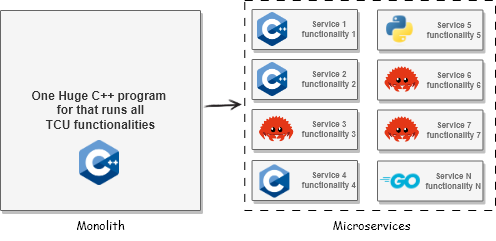
\includegraphics[scale=0.7]{Figures/14.png}
\caption[Microservices vs Monolithic approach]{Microservices vs Monolithic approach}
\label{fig:Micro_service_vs_monolith}
\end{figure}

In the context of embedded systems, where High Power System-on-Chips (SoCs) like the raspberry pi 4B in our case with Linux operating systems are used, the microservices approach can provide several advantages over a monolithic architecture. Let's explore how microservices excel in this domain:
Modularity: Embedded systems often require a high degree of modularity due to the complexity of the hardware and software components involved. Microservices offer a modular approach where each service can be developed, tested, and deployed independently. This modularity enables easier maintenance and extensibility of the system. If a specific functionality or service needs to be updated or replaced, it can be done without affecting the rest of the system.
Resource Efficiency: High Power SoCs in embedded systems often come with significant computational capabilities and memory resources. With a microservices architecture, these resources can be effectively utilized. Each microservice can be allocated resources based on its specific requirements, enabling fine-grained resource management. In a monolithic architecture, the entire application shares the same resources, which might not be efficiently utilized for different components.
Customizability and Flexibility: Embedded systems often require customization to suit specific application requirements. With microservices, different components of the system can be developed using different technologies and programming languages. This flexibility allows developers to choose the most suitable tools for each service, optimizing performance, and reducing development constraints. In a monolithic architecture, the entire system is built using a single technology stack, limiting customization options. As visualized in (figure9).
System Partitioning: Microservices enable the partitioning of the embedded system into logical components, each responsible for a specific functionality. This partitioning allows for better management and separation of concerns. Developers can focus on specific services independently, facilitating easier debugging, testing, and maintenance.
\subsection{Microservices Architecture in SDV}
One of the key advantages of microservices architecture is its container-based nature, which abstracts the underlying hardware and provides several benefits when it comes to deploying and updating applications, as visualized in (figure1). Containers provide a consistent and isolated environment for running microservices. Each microservice can be packaged into its own container, along with its dependencies and runtime environment. This ensures that the application behaves consistently across different deployment environments, regardless of the underlying hardware or operating system. Containers encapsulate the entire runtime environment, including the application and its dependencies. This makes microservices highly portable, allowing them to be easily deployed across different infrastructure platforms, such as local development machines, cloud environments, or edge devices that follow the SOAFEE architecture, as visualized in \ref{fig:SOAFEE Architecture}. The abstraction of hardware details allows developers to focus on building and testing the application logic rather than worrying about compatibility issues across various hardware configurations.
\begin{figure}[!ht]
\centering
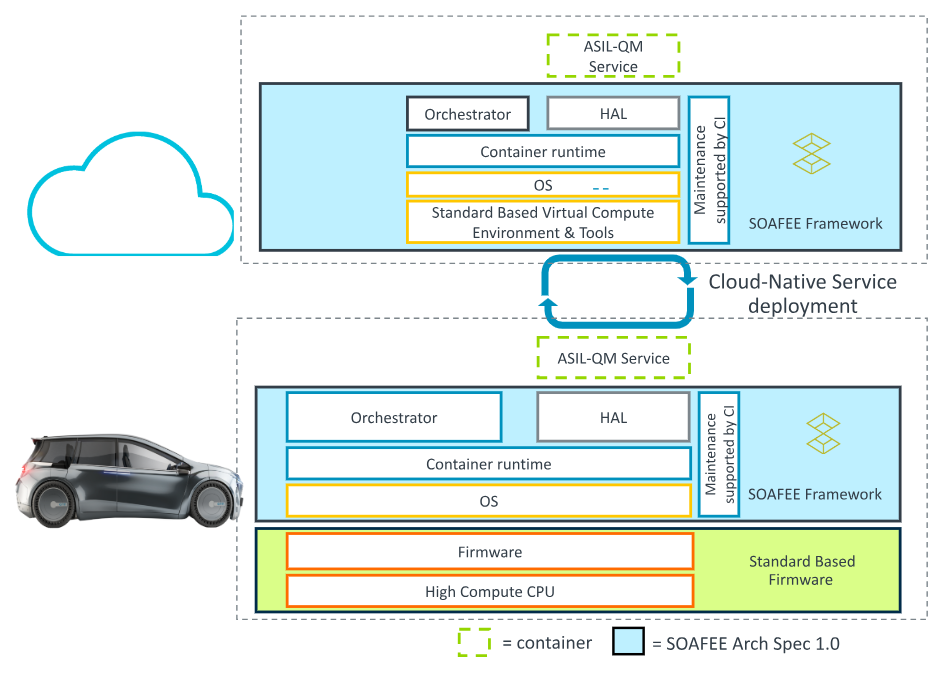
\includegraphics[scale=0.4]{Figures/15.png}
\caption[SOAFEE Architecture]{SOAFEE Architecture}
\label{fig:SOAFEE Architecture}
\end{figure}

\clearpage

\section{Docker Compose}
Docker Compose is a powerful tool that simplifies the deployment and management of multi-container applications. While its usage is prevalent in server applications, Docker Compose also brings significant benefits to embedded systems.

In the context of embedded systems, Docker Compose scripts offer a convenient way to package and deploy complex applications composed of multiple interconnected components. By defining the services, networks, and volumes required to run and connect various Docker containers in a single YAML file, Docker Compose streamlines the deployment process. This allows for easy replication and distribution of the entire application setup across different embedded systems.

One of the key advantages of Docker Compose in embedded systems is its support for application modularity and scalability. By defining each component of the system as a separate container, Docker Compose promotes a modular approach. Each container encapsulates a specific functionality or component, enabling easy scaling or replacement of individual services without impacting the entire application. This flexibility is particularly valuable in embedded systems, where resource constraints and varying software requirements often necessitate granular control over application components.

Dependency management is another area where Docker Compose proves beneficial in embedded systems. With embedded systems often relying on multiple software components and libraries, Docker Compose allows for the precise definition and management of dependencies within their respective containers. This simplifies the process of managing dependencies and reduces the likelihood of conflicts between different software components, ensuring smooth operation of the overall system. Example of a docker compose file in figure \ref{fig:docker_compose_script}.


\begin{figure}[h]
\centering

\includegraphics[scale=0.4]{Figures/17.png}
\caption[docker compose logo]{docker compose logo}
\label{fig:docker_compose_logo}
\end{figure}

\clearpage

\begin{figure}[h]
\centering
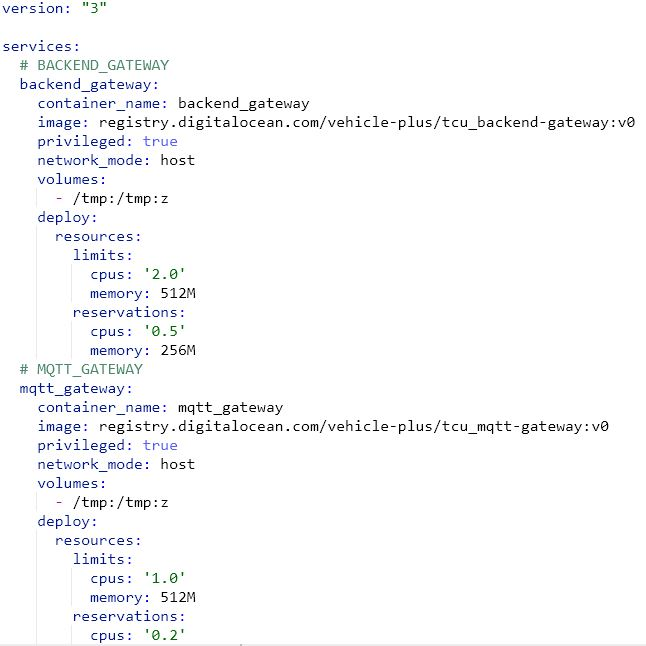
\includegraphics[scale=0.6]{Figures/docker_compose_script.JPG}
\caption[docker compose script]{example of docker compose script}
\label{fig:docker_compose_script}
\end{figure}

\section{VSOME/IP}
\subsection{SOME/IP Overview}
SOME/IP \cite{ioana2020opc}, short for "Scalable service-Oriented middlewarE over IP," is a middleware specifically developed for automotive applications and designed to be compatible with AUTOSAR (at least at the wire-format level). A comprehensive specification for SOME/IP can be accessed publicly at \url{http://some-ip.com/} \cite{SOME/IP}. The specification encompasses three key components:
\begin{itemize}
\item On-wire format
\item Protocol
\item Service Discovery
\end{itemize}

\subsection{SOME/IP On-wire format}
\begin{figure}[!ht]
\centering
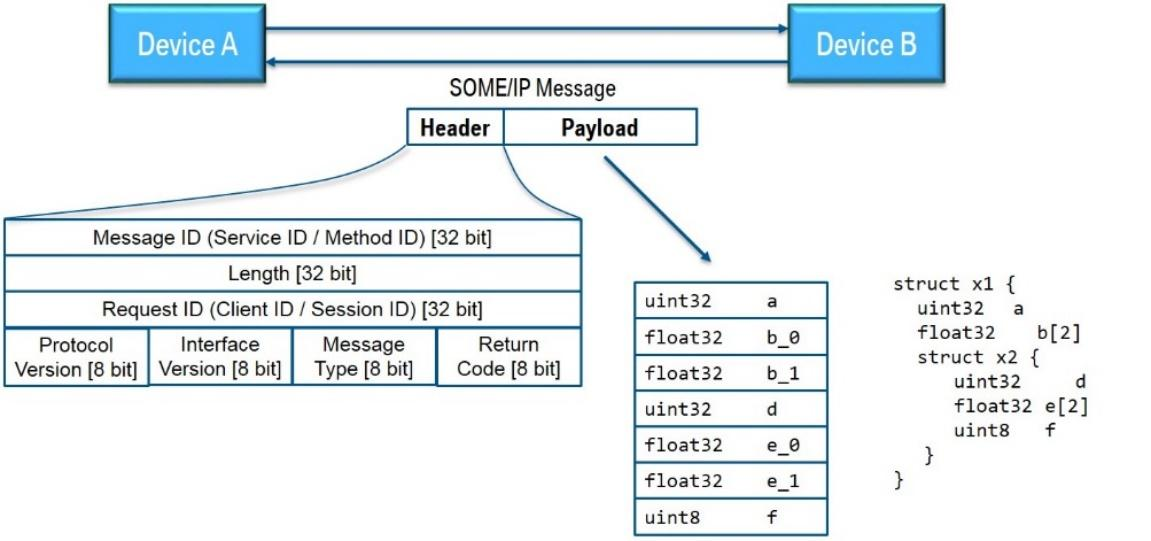
\includegraphics[scale=0.3]{Figures/18.png}
\caption[SOMEIP message sent from Device A to Device B]{SOME/IP message sent from Device A to Device B}
\label{fig:SOME/IP On-wire format}
\end{figure}


In the given scenario, we have two devices, Device A and Device B. Device A sends a SOME/IP message to Device B and expects to receive a response. The underlying transport protocol can be either TCP or UDP, but this choice does not affect the content of the message.

The SOME/IP messages consist of two main parts: the header and the payload. The header primarily contains identifiers that help in message processing. These identifiers include:

\begin{enumerate}
\item Service ID: A unique identifier for each service.
\item Method ID: Ranging from 0 to 32767 for methods and from 32768 to 65535 for events.
\item Length: Indicates the length of the payload in bytes, including the next identifiers (8 additional bytes).
\item Client ID: A unique identifier for the calling client within the Electronic Control Unit (ECU). It must be unique throughout the entire vehicle.
\item Session ID: An identifier used for session handling. It should be incremented for each call.
\item Protocol Version: Set to 0x01.
\item Interface Version: The major version of the service interface.
\item Message Type: Specifies the type of message being sent.
\item Return Code: Indicates the result of the message exchange.
\end{enumerate}
The payload of the SOME/IP message contains serialized data. In the provided illustration (Figure 19), the serialization is demonstrated for a simple case where the transmitted data structure consists of nested structures with only basic data types. In this scenario, the struct elements are flattened and written sequentially into the payload. Therefore, in the given communication setup, Device A sends a SOME/IP message to Device B, including the necessary identifiers in the header and the serialized data in the payload. Device B processes the message and sends back a response message if required. Additionally, errors can be reported as responses with the return code indicating the specific error encountered.


\subsection{SOME/IP Protocol}
\begin{figure}[!ht]
\centering
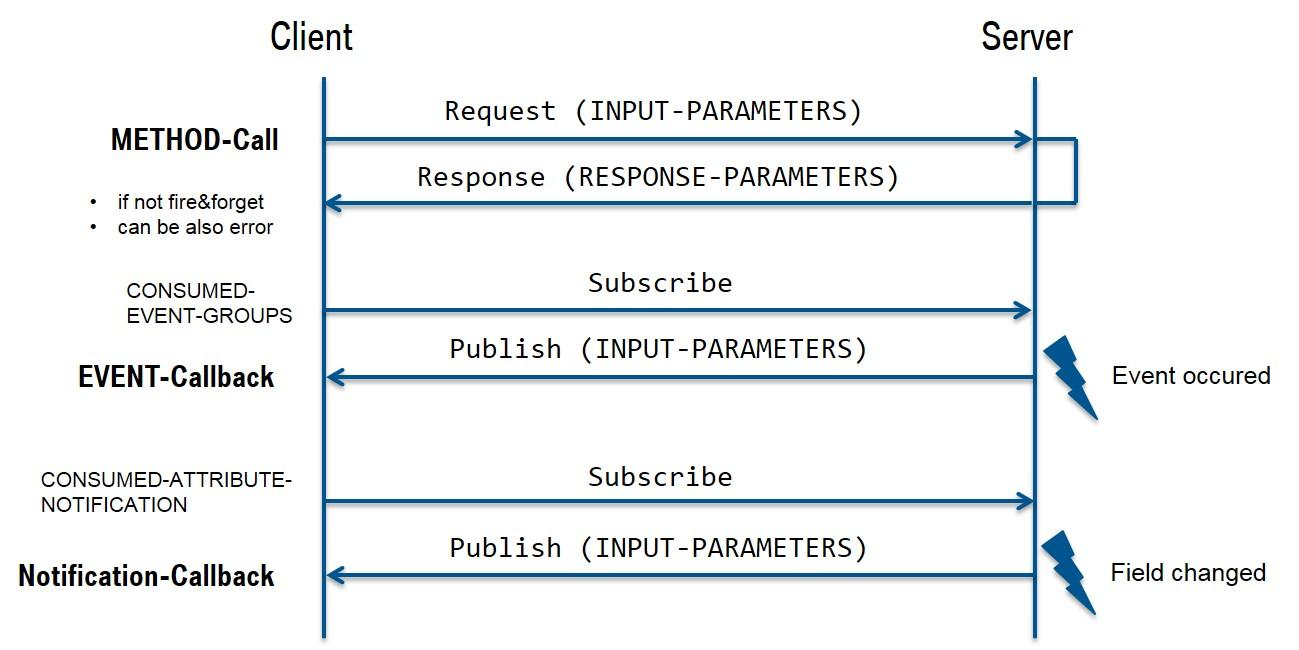
\includegraphics[scale=0.3]{Figures/19.png}
\caption[SOME/IP communication patterns]{SOME/IP communication patterns}
\label{fig:TCU}
\end{figure}
The SOME/IP specification supports two transport bindings: UDP and TCP. These bindings facilitate communication between systems using basic communication patterns, namely publish/subscribe and request/response. In the UDP transport binding, SOME/IP messages are not fragmented. It is possible to have multiple messages within a single UDP packet, but each individual message cannot exceed the maximum size allowed for a UDP package (up to 1400 bytes). If a message exceeds this limit, it must be transported using TCP. In the UDP case, the SOME/IP specification does not utilize the robustness features of TCP.
When TCP is used as the transport protocol, all the robustness features provided by TCP are employed. TCP ensures reliable and ordered delivery of messages between systems. If a synchronization error occurs within the TCP stream, the SOME/IP specification allows the use of "magic cookies." These magic cookies serve as markers to identify the beginning of the next message, allowing for proper message parsing and processing.
In addition to the standard REQUEST/RESPONSE mechanism for remote procedure calls the SOME/IP protocol also uses the PUBLISH/SUBSCRIBE pattern for events as visualized in (figure19).
\subsection{SOME/IP Service Discovery}
\begin{figure}[!ht]
\centering
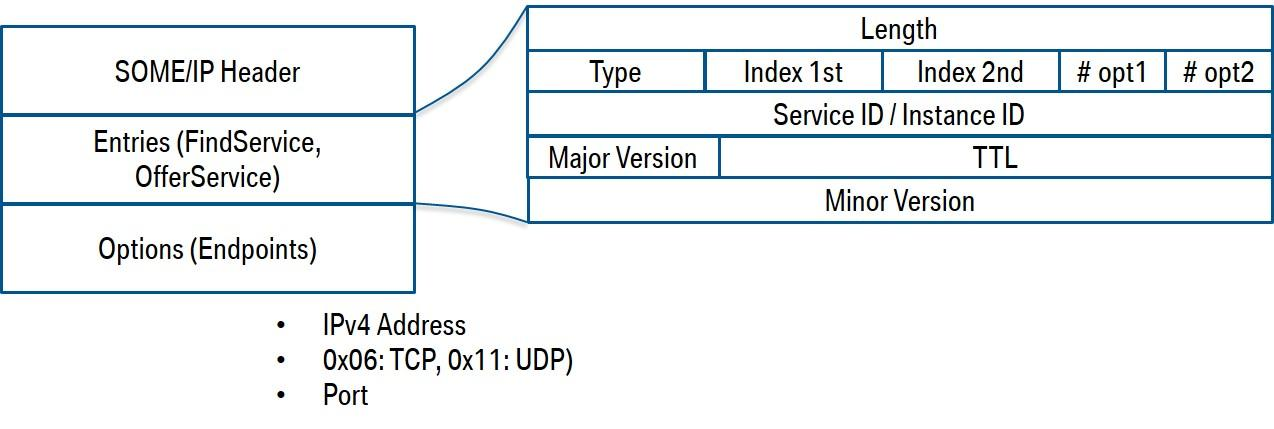
\includegraphics[scale=0.3]{Figures/20.png}
\caption[Structure of SOME/IP service discovery message]{Structure of SOME/IP service discovery message}
\label{fig:TCU}
\end{figure}

SOME/IP Service Discovery used to locate service instances and to detect if service instances are running, determining their availability, and implementing the Publish/Subscribe functionality. This is achieved primarily through the use of "offer messages." Each device broadcasts or multicasts messages that contain information about the services it offers. These offer messages facilitate the discovery of available services across the network.
The communication of SOME/IP Service Discovery messages occurs via UDP, providing a lightweight and efficient means of transmission. By using UDP, devices can efficiently exchange the necessary information for service discovery without the need for additional overhead introduced by TCP. In cases where client applications require specific services that are currently not being offered, "find messages" can be sent to actively search for those services. These find messages help in identifying devices that provide the desired services and enable clients to establish connections accordingly.
Additionally, other SOME/IP Service Discovery messages are utilized for publishing or subscribing to an event group. These messages enable devices to announce the availability of event groups or to express interest in receiving notifications related to specific event groups.
\subsection{VSOME/IP}
\subsubsection{Adopted implementation}
In the TCU we used the implementation provided from GENEVI which is called VSOME/IP.
For more information about VSOME/IP you can check the open-source implementation to the VSOME/IP on GitHub at https://github.com/COVESA/VSOME/IP 
VSOME/IP encompasses not only the external communication between devices but also internal inter-process communication which what we used strongly on the inter-service communication inside the TCU.
 The communication between two devices occurs through communication endpoints, which determine the transport protocol (TCP or UDP) and associated parameters such as port numbers. These parameters are configurable and can be set in a VSOME/IP configuration file, typically in JSON format as outlined in the VSOME/IP user guide.
For internal communication, VSOME/IP employs local endpoints implemented using Unix domain sockets and the Boost.Asio library. This approach enables fast and efficient communication within the system. Unlike centralized systems like the D-Bus daemon, internal communication in VSOME/IP does not require routing through a central component, resulting in improved performance.
\begin{figure}[!ht]
\centering
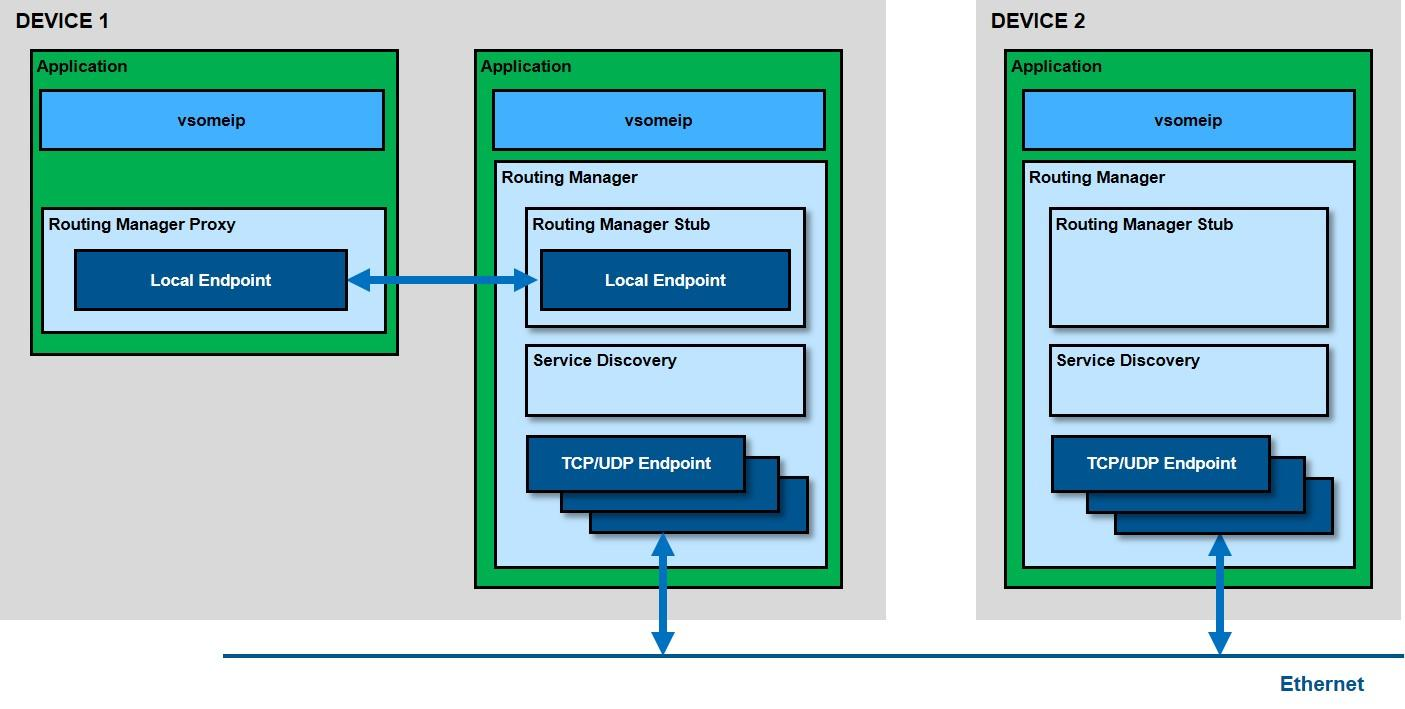
\includegraphics[scale=0.3]{Figures/21.png}
\caption[VSOME/IP communication IPC and with different devices]{VSOME/IP communication IPC and with different devices}
\label{fig:TCU}
\end{figure}


By utilizing communication endpoints and local endpoints with Unix domain sockets, VSOME/IP facilitates both external and internal communication in an efficient and configurable manner. This design allows for seamless communication between devices while maintaining high-speed inter-process communication within the system.

\subsection{Services communication using VSOME/IP}
\subsubsection{VSOME/IP with containerized services}
\begin{figure}[!ht]
\centering
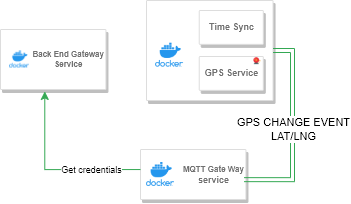
\includegraphics[scale=0.8]{Figures/22.png}
\caption[Different Services communicate using PUB/SUB and RPC using VSOME/IP IPC]{Different Services communicate using PUB/SUB and RPC using VSOME/IP IPC}
\label{fig:TCU}
\end{figure}
In the TCU each service within our system is designed with specific functionalities to fulfill different requirements as visualized in (figure16). For instance, the backend gateway service handles communication with the backend server by utilizing HTTP requests and establishing a secure channel for data transfer. On the other hand, the MQTT gateway service functions as an MQTT client, enabling it to publish messages to and subscribe to various MQTT topics. Additionally, the GPS service is responsible for acquiring data from the GNSS module through UART serial communication.
To facilitate seamless communication and meet the overall system requirements, all services utilize the VSOME/IP stack. The VSOME/IP stack serves as a communication framework that allows services to interact with each other effectively. This integration ensures efficient data exchange and coordination among the services, enabling the system to function harmoniously. 
In this scenario (Figure 16), the MQTT Gateway invokes a method provided by the Backend Gateway service to retrieve credentials. Additionally, the MQTT Gateway subscribes to an event provided by the GPS service. Whenever the GPS service triggers that event, the MQTT Gateway receives notifications containing the published data associated with the event.

\subsubsection{Containerizing service with VSOME/IP}

In the project we use VSOME/IP with containers using this procedure create a Docker file using the Alpine image as the base building image. Within this file, we will include the necessary steps to build the Boost Library, as it is required for the VSOME/IP library. Afterwards, we will proceed to build the VSOME/IP library specifically for this container. Additionally, we will designate the (/tmp) directory as a shared volume for the container, allowing it to utilize the Unix domain socket.

To access more information about our implementation, please scan the QR code provided. It will provide you with detailed insights and details regarding our implementation.

\begin{figure}[!ht]
\centering

\includegraphics[scale=1]{Figures/Vehicle_Plus_VsomeIp_repo.png}
\caption[Vehicle plus Implementation to VSOME/IP]{Vehicle plus Implementation to VSOME/IP}
\label{fig:SOME/IP On-wire format}
\end{figure}


\chapter{TCU Applications and System Services}
\section{Services Layout}
\begin{figure}[h]
\centering
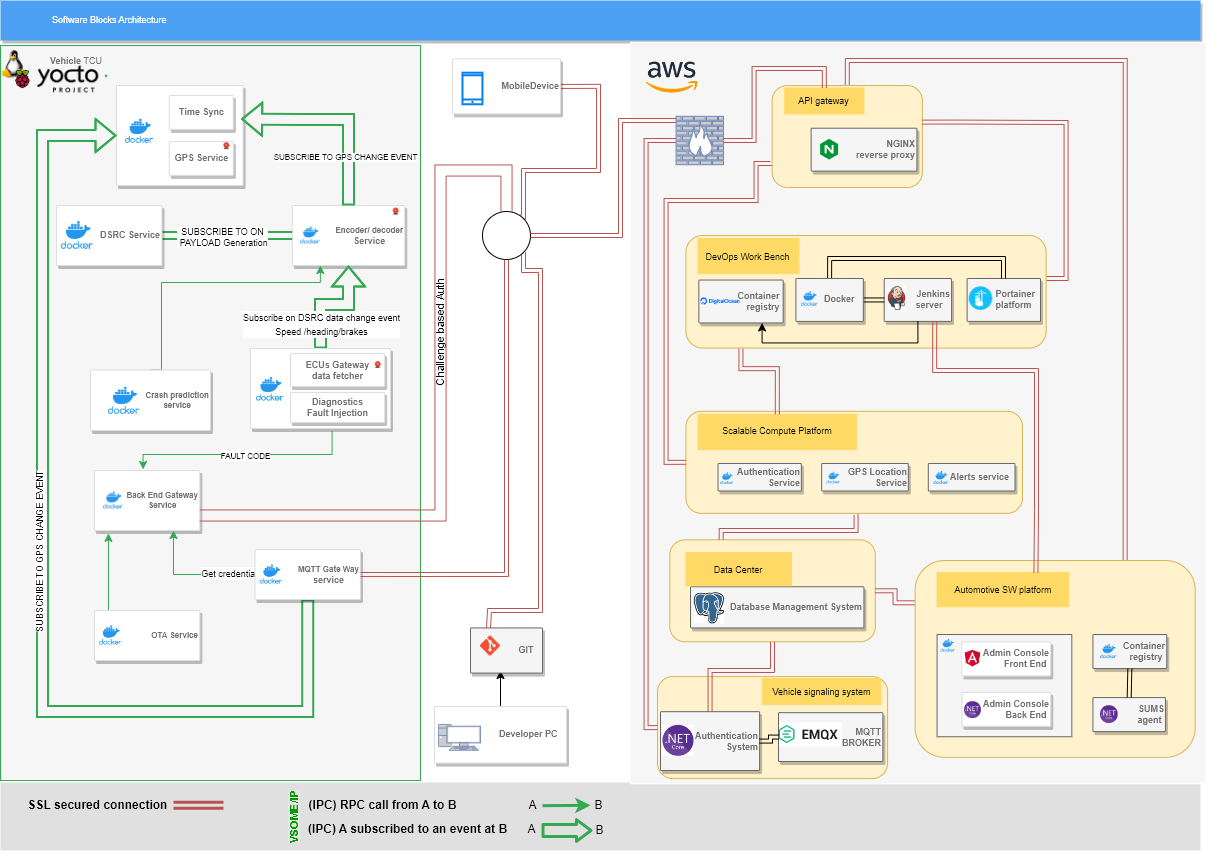
\includegraphics[scale=0.38]{Figures/23.png}
\caption[TCU Containerized Services Layout]{TCU Containerized Services Layout}
\label{fig:TCU Containerized Services Layout}
\end{figure}
The diagram in \ref{fig:TCU Containerized Services Layout} depicts the containerized services running on the TCU along with their interactions. You can see the various services encapsulated within containers, and their connections and communication with each other.
On the right side of the diagram, the services running on the Cloud are illustrated. These services operate separately from the TCU and have their own interactions. They interact not only with each other but also establish secure connections with the TCU over the internet. The diagram shows the flow of information and interactions between the Cloud services and the TCU services.
To summarize previous sections the system is composed of multiple services, each of which operates within its own containerized environment. The Docker engine is utilized to manage and control all of these containers. This design allows for efficient isolation and management of individual services. Communication between the containers is facilitated using VSOME/IP, a communication stack. Two approaches for communication within this architecture are RPC (Remote Procedure Call) calls and the publish/subscribe paradigm. RPC calls enable services to invoke methods on other services residing in different containers. This synchronous communication mechanism allows for direct interaction between services, making it useful for scenarios where immediate responses are required. On the other hand, the publish/subscribe paradigm allows for asynchronous communication. Services can publish messages or events to specific topics, and other services that have subscribed to those topics will receive the messages. This decoupled communication style is well-suited for scenarios where services need to be loosely coupled and independent, enabling them to react to events or messages at their own pace. By leveraging the combination of containerization with the Docker engine and using VSOME/IP for inter-container communication, the system achieves enhanced modularity, scalability, and flexibility.
Each service can be independently deployed, updated, or scaled, facilitating efficient development and deployment processes. Additionally, the choice of RPC calls or publish/subscribe paradigm enables the system to accommodate different communication patterns based on the requirements of specific services or use cases.

\section{Backend Gateway Service}
\begin{figure}[!ht]
\centering
\begin{minipage}{0.45\textwidth}
  \centering
  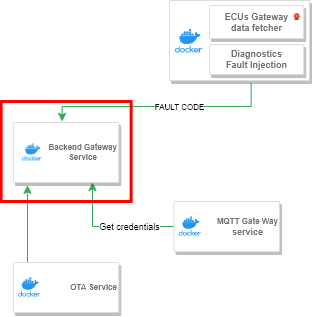
\includegraphics[width=\linewidth]{Figures/24.png}
  \caption[Backend Gateway Service]{Backend Gateway Service}
  \label{fig:Backend Gateway Service}
\end{minipage}\hfill
\begin{minipage}{0.45\textwidth}
  \centering
  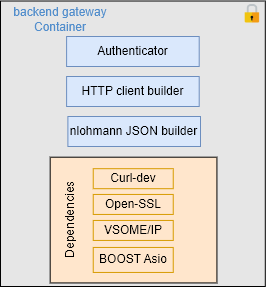
\includegraphics[width=\linewidth]{Figures/25.png}
  \caption[Backend gateway container]{Backend gateway container}
  \label{fig:Backend Gateway container}
\end{minipage}
\end{figure}
The implementation of the backend gateway is on GitHub you can scan the following QR code to get to the source code of the backend gateway.

\begin{figure}[!ht]
\centering

\includegraphics[scale=1]{Figures/backend_gateway_QR.png}
\caption[Backend gateway QR code]{Backend gateway QR code}
\label{fig:SOME/IP On-wire format}
\end{figure}


The Backend Gateway Service, operating on the Telematics Control Unit (TCU), acts as a communication bridge between the TCU and the Backend Server. It employs an HTTP-Builder to generate HTTP requests, facilitating seamless data exchange with the Backend Server. To ensure secure transmission, the Backend Gateway Service establishes an SSL connection using the Open-SSL library, thereby safeguarding the communication between the TCU and the Backend Server located in the cloud. 
A pivotal responsibility of the Backend Gateway is to handle the transmission of various types of HTTP requests, including POST, GET, and PUT, from the TCU to the Backend Server. As part of the authentication process, the Backend Gateway undergoes challenge-based authentication with the Backend Server. Upon successful authentication, the Backend Server issues a JSON Web Token (JWT) to the TCU, granting it access for a specific time period. Subsequently, the Backend Gateway Service utilizes this token to send subsequent requests to the Backend Server.
Maintaining security and access control, the Backend Gateway Service actively monitors the validity of the JWT token. When the token expires or becomes invalid, it is responsible for re-authenticating itself with the Backend Server, ensuring uninterrupted and authorized access.

\subsection{Offered Services}
The backend gateway provides a VSOME/IP service that allows external services running on the TCU to send POST requests to the backend server securely. These requests contain specific data in JSON format, which is then transmitted to the backend server. The service is identified by the following parameters: SERVICE\_ID (0x1234), INSTANCE\_ID (0x5678), and METHOD\_ID (0x0421).

\subsection{Challenge based authentication}
Implementing TCU authentication in our project posed a significant challenge due to its unique requirements and criticality within the automotive domain. Unlike traditional authentication schemes, TCU authentication involves automatic identification and registration of vehicles without any user intervention. Moreover, the level of criticality associated with automotive authentication is considerably higher, as it directly impacts the security of a system considered a human safety critical system. To address these challenges, extensive research and a combination of multiple techniques were employed to provide robust and secure functionality.

One of the key aspects of TCU authentication is the automatic identification of vehicles. This involves implementing techniques such as digital certificates, secure protocols, and cryptographic algorithms to enable secure and automatic identification of vehicles. Digital certificates provide a means to establish the authenticity and trustworthiness of the vehicle, while secure protocols ensure the integrity and confidentiality of the communication between the TCU and the authentication system.

Additionally, a robust registration process had to be developed to facilitate automatic registration of vehicles on the system. This process involves securely exchanging and verifying vehicle credentials, such as vehicle identification numbers (VINs), manufacturer-specific data, and other unique identifiers. These credentials are used to authenticate the vehicle and establish a secure and trusted connection with the system.

To ensure the high level of criticality required for automotive authentication, multiple layers of security were implemented. This includes secure storage and handling of credentials, strong encryption algorithms, and strict access controls. Access to the authentication system is tightly regulated, with role-based access control and strict authentication policies in place to prevent unauthorized access and mitigate potential security threats.



In our solution, the TCU initiates the authentication process by requesting a challenge from the server. The challenge is a stream of bytes encrypted using the public key from the chained certificate, ensuring that only the corresponding private key held by the TCU can decrypt it. This challenge serves as a one-time passphrase that can be used for authentication. Upon receiving the encrypted challenge, the TCU decrypts it using its private key, generating the one-time passphrase. This passphrase, combined with the chained certificate, is then used to initiate the login process on the server. The server, upon receiving the login request, verifies the authenticity of the TCU by checking the MAC address embedded in the certificate. This MAC address serves as a unique identifier for the vehicle, confirming its identity and preventing unauthorized entities from accessing the server.

\begin{figure}[!ht]
\centering
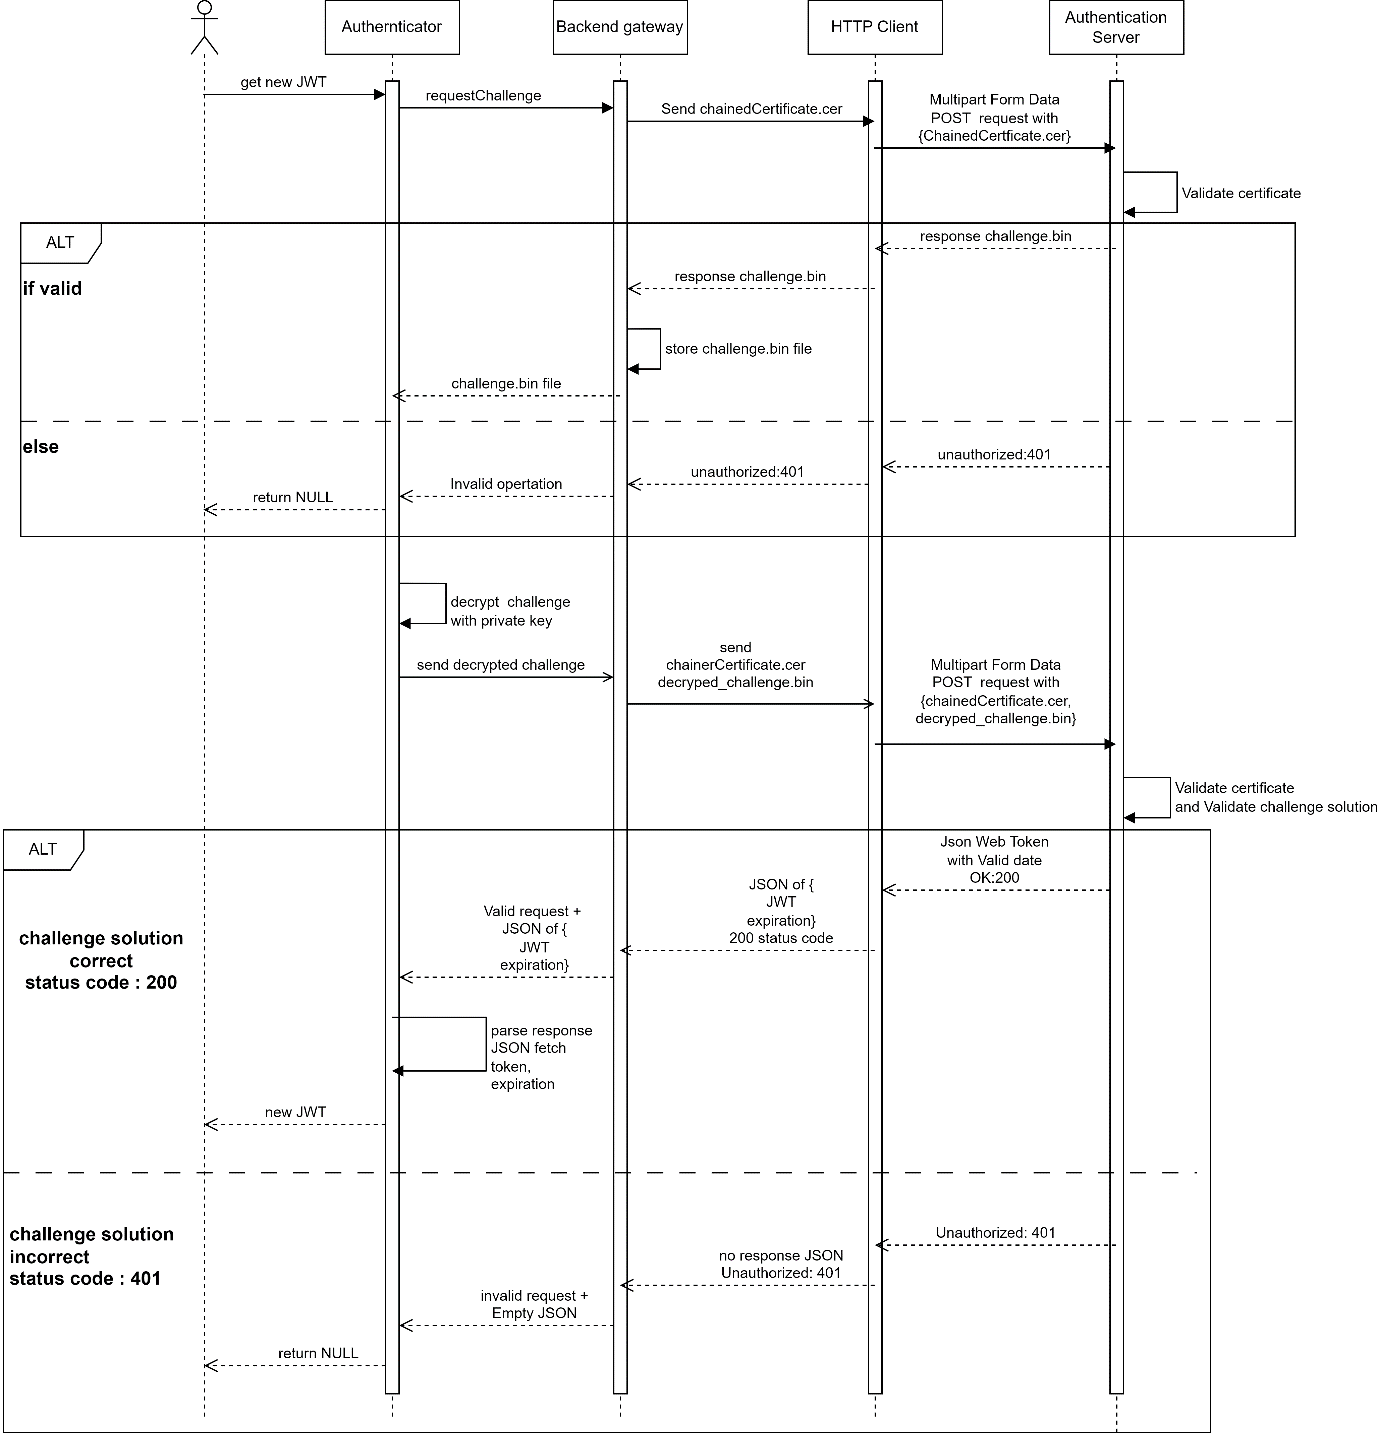
\includegraphics[scale=0.33]{Figures/26.png}
\caption[Authentication UML sequence diagram]{Authentication UML sequence diagram}
\label{fig:TCU}
\end{figure}

\clearpage

By employing challenge-based authentication, our system ensures that only the TCU possessing the private key linked to the public key used in generating the CSR can successfully decrypt the challenge and provide the corresponding passphrase. This approach provides a strong level of assurance in the authentication process and safeguards against unauthorized access to the server. The combination of chained certificates, MAC address verification, and challenge-based authentication establishes a robust and secure mechanism for TCU authentication within our cloud-based system.




\section{ECUs Gateway Data Fetcher}
\subsection{Introduction}
The ECUs Gateway Data Fetcher Service plays a pivotal role in the overall system as a containerized service running on a TCU (Raspberry Pi), harnessing the power of Docker. Utilizing the Boost ASIO library, this service is dedicated to listening on port 5001, eagerly awaiting UDP connections from diverse sources. By leveraging the capabilities of the Boost ASIO library and operating at this low-level network protocol, the ECUs Gateway Data Fetcher Service establishes a direct and efficient channel of communication with other essential components of the system.

The TCU, acting as the central hub, seamlessly integrates with multiple Electronic Control Units (ECUs) through an Ethernet network. With each ECU serving a specific purpose, tailored to contribute precise information crucial for the system's optimal operation, the ECUs Gateway Data Fetcher Service becomes the vital interface for collecting and processing the data transmitted by these ECUs.

\begin{figure}[!ht]
\centering
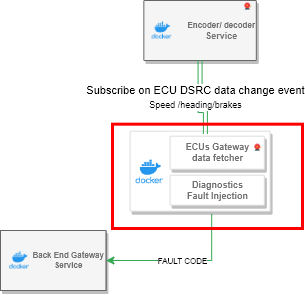
\includegraphics[scale=0.5]{Figures/27.png}
\caption[ECUS gateway data fetcher]{ECUS gateway data fetcher}
\label{fig:ECUS gateway data fetcher}
\end{figure}
\subsubsection{Purpose of The Service}
The ECUs Gateway Data Fetcher Service plays a crucial role in the overall system by providing essential monitoring and diagnostic capabilities. Its purpose and significance can be understood through the following subpoints:

\begin{itemize}
  \item Real-time Monitoring and Alerting: One of the primary purposes of the ECUs Gateway Data Fetcher Service is to enable real-time monitoring and alerting. By seamlessly integrating with a mobile application, the service facilitates the delivery of real-time notifications to users' mobile devices. These notifications serve as a direct means of keeping users informed about the system's diagnostics and status. In the event of critical events or anomalies within the system, such as battery issues, tire pressure abnormalities, or headlight malfunctions, the service promptly generates notifications and transmits them securely to the mobile application. This timely dissemination of information empowers users to stay up to date with the system's performance and take appropriate actions promptly, thereby ensuring optimal system operation and user satisfaction.
  
  \item DSRC Message Notifications: The ECUs Gateway Data Fetcher Service includes a powerful notification mechanism specifically designed to inform clients about updates related to DSRC (Dedicated Short Range Communications) messages. DSRC message notifications are particularly significant as they provide crucial information about speed and heading. By subscribing to these notifications, clients gain access to real-time updates regarding their vehicle's speed and precise heading. This feature enables clients to make informed decisions based on the latest data, supporting crucial decision-making processes related to adaptive cruise control, collision warning systems, and other advanced functionalities. The ability to receive DSRC message notifications in real-time empowers clients to optimize their driving experience, enhance safety measures, and leverage the full potential of the system.
  
  \item Scalability and Extensibility: The ECUs Gateway Data Fetcher Service is designed to be scalable and extensible, capable of handling increasing data volumes and accommodating new diagnostic requirements. It can adapt to evolving system architectures and accommodate additional monitoring sources. This scalability and extensibility ensure that the service remains effective and valuable as the system grows and evolves over time.
\end{itemize}

\subsection{Types of Messages}
The ECUs fulfill various roles such as monitoring and reporting speed, accurately determining the vehicle's heading, and providing critical diagnostic messages. Within the realm of diagnostic messages, the ECUs Gateway Data Fetcher Service recognizes two distinct types: DSRC (Dedicated Short Range Communications) messages and Diagnostic messages. Each type carries valuable insights into the vehicle's health and functionality.

\begin{itemize}
  \item DSRC Messages:
  \begin{enumerate}
    \item Speed Message: This message provides real-time updates on the vehicle's speed. It is crucial for various decision-making processes, such as adaptive cruise control or collision warning systems.
    \item Heading Message: This message conveys information about the vehicle's precise heading. It is essential for navigation systems, adaptive cruise control, or collision warning systems.
  \end{enumerate}

  \item Diagnostic Messages:
  \begin{enumerate}
    \item Battery Message: This message assesses the battery's current condition. By carefully analyzing the battery message, the service determines whether the battery level is dangerously low or if it remains in an acceptable range, ensuring the vehicle's reliability.
    \item Tyre Pressure Message: This message provides crucial details regarding tire pressure. The ECUs Gateway Data Fetcher Service diligently inspects this message to determine whether the tire pressure is below the recommended threshold, warranting immediate attention, or if it remains at an optimal level, guaranteeing a safe and smooth ride.
    \item Headlight Condition Message: This message concerns the functionality of the vehicle's headlights. By meticulously examining this message, the ECUs Gateway Data Fetcher Service ascertains whether any faults or malfunctions exist in the headlights, enabling prompt maintenance or replacements, thus ensuring the safety of the vehicle and its occupants.
  \end{enumerate}
\end{itemize}

To effectively categorize and process these diagnostic messages, the ECUs Gateway Data Fetcher Service relies on the source port associated with each UDP connection. This intelligent parsing mechanism allows the service to accurately identify the type of message received and facilitates further analysis and appropriate actions. Messages related to the vehicle's speed are identified through a source port value of 6000, while a source port of 6001 corresponds to messages pertaining to the vehicle's precise heading. Similarly, a source port of 6002 indicates the presence of a tire message, and a source port of 6003 signifies a battery message. Lastly, a source port of 6004 denotes the arrival of a headlight message. By leveraging these source port identifiers, the ECUs Gateway Data Fetcher Service efficiently processes the diagnostic messages, ensuring precise categorization.

\subsection{VSOME/IP Usage}
\subsubsection{RPC}
The Diagnostics + UDP Server Service not only fulfills its role as a diagnostic message receiver but also leverages advanced technologies to enhance its functionality and integration within the system. One such technology employed by the service is VSOMEIP, which enables seamless communication and interaction among various components of the system. Through VSOMEIP, the Diagnostics + UDP Server Service is able to invoke a function within the backend-gateway service, initiating a POST request to transmit the essential diagnostic information. This request carries the valuable insights gathered from the diagnostic messages and is directed towards the backend server, ensuring the proper storage and further processing of the data. This integration of VSOMEIP and RPC mechanisms facilitates comprehensive analysis and decision-making based on the rich diagnostic insights obtained.

\subsubsection{Subscribe/Notify}
The ECUs Gateway Data Fetcher Service incorporates a powerful subscribe/notify mechanism that enhances its functionality and interconnectivity within the system. This feature allows clients to subscribe to updates related to heading and speed, receiving timely notifications whenever changes occur. One notable client that benefits from this mechanism is the DSRC service. By promptly notifying the DSRC service of any updates in the vehicle's heading and speed, the ECUs Gateway Data Fetcher Service ensures the availability of real-time data for crucial decision-making processes. This synchronization between the ECUs Gateway Data Fetcher Service and the DSRC service empowers the system to make informed and responsive decisions based on the most up-to-date information, contributing to enhanced safety and performance.
\begin{figure}[!ht]
\centering
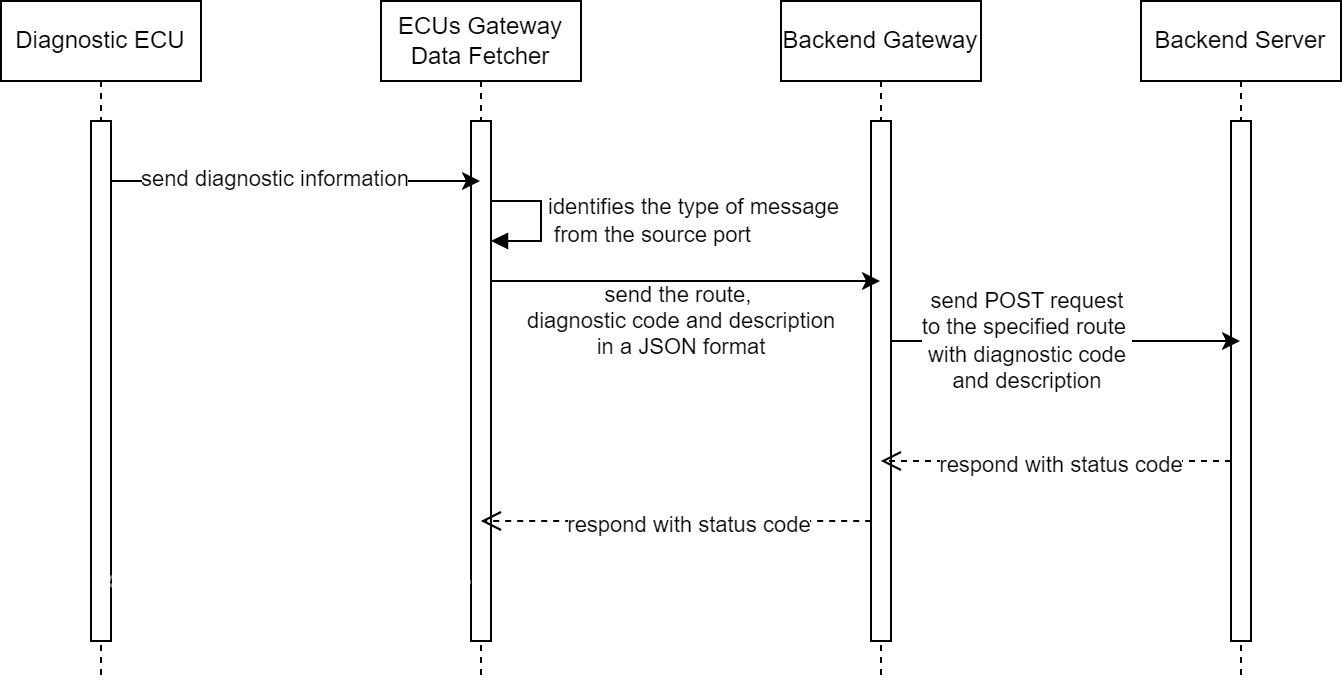
\includegraphics[scale=0.4]{Figures/28.png}
\caption[ECU Gatway pub/sub]{ECU Gatway pub/sub}
\label{fig:TCU}
\end{figure}
\begin{figure}[!ht]
\centering
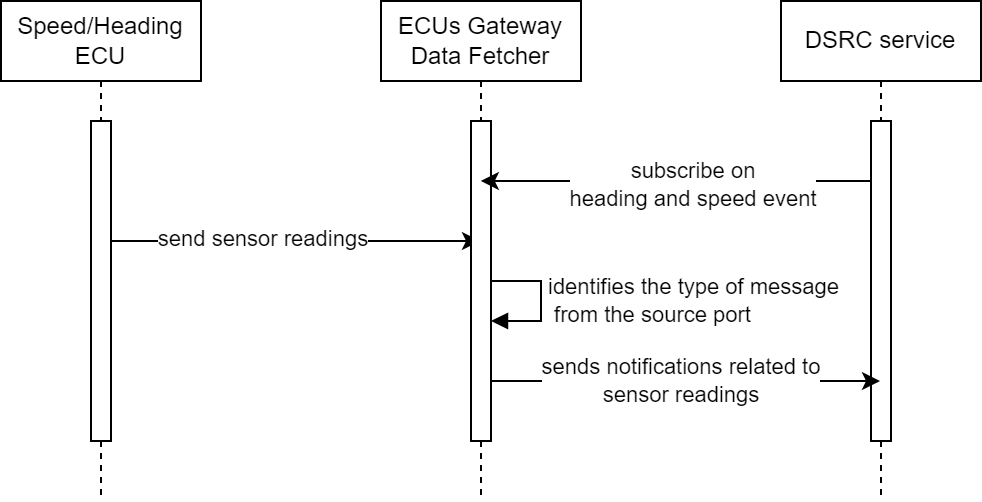
\includegraphics[scale=0.4]{Figures/29.png}
\caption[DSRC withECU Gatway pub/sub]{DSRC withECU Gatway pub/sub}
\label{fig:TCU}
\end{figure}
\subsection{Conclusion}
In conclusion, the ECUs Gateway Data Fetcher Service plays a vital role in the overall system by providing essential monitoring and diagnostic capabilities. It seamlessly integrates with multiple ECUs, serving as the interface for collecting and processing crucial data transmitted by these components. The service enables real-time monitoring and alerting, delivering notifications to users' mobile devices to keep them informed about the system's diagnostics and status. Additionally, the service incorporates a powerful notification mechanism specifically designed to provide DSRC message updates, including speed and heading, allowing clients to make informed decisions based on real-time data.
The ECUs Gateway Data Fetcher Service demonstrates its scalability and extensibility, capable of accommodating increasing data volumes and evolving system architectures. Its integration with advanced technologies like VSOMEIP and RPC mechanisms enhances its functionality and enables comprehensive analysis and decision-making based on the rich diagnostic insights obtained. The service's ability to subscribe/notify clients, particularly the DSRC service, ensures real-time data availability for critical decision-making processes, contributing to enhanced safety and performance.

\section{DSRC Encoder/Decoder}
\begin{figure}[!ht]
\centering
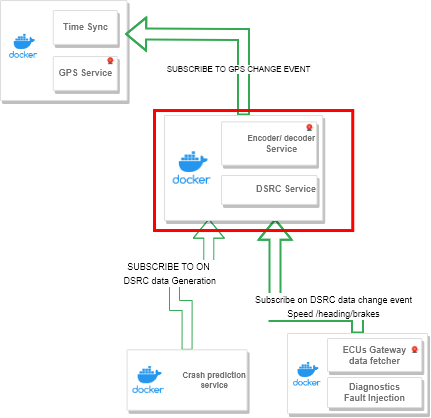
\includegraphics[scale=0.5]{Figures/30.png}
\caption[DSRC Encoder/Decoder service]{DSRC Encoder/Decoder service}
\label{fig:DSRC Encoder/Decoder}
\end{figure}
The Encoder/Decoder software serves as a crucial component in the communication infrastructure of vehicles, operating on the Raspberry Pi platform. Its primary function is to facilitate seamless communication between vehicles by interacting with the Dedicated Short-Range Communications (DSRC) module, which is responsible for broadcasting and receiving payload messages. Additionally, the software receives data from the vehicle's sensors using the Vehicle Service Oriented Middleware over Internet Protocol (VSOMEIP) protocol. This article explores the features and functionalities of the Encoder/Decoder software, highlighting its role in capturing, storing, and transmitting sensor data efficiently.

\subsection{Communication and Integration: The Encoder/Decoder's Role}
The Encoder/Decoder software acts as a vital intermediary between the DSRC module and the vehicle's sensors. Its purpose is to establish and maintain communication channels for transmitting data and payload messages. By constantly monitoring the VSOMEIP services associated with various vehicle sensors, the Encoder/Decoder remains in a ready state to receive notifications from any relevant service. This ensures that all sensor readings can be efficiently captured and processed.

\subsection{Sensor Data Capture and Storage: The Payload Stack}
To store the received sensor readings, the Encoder/Decoder employs a stack-based approach known as the payload stack. This stack serves as a dedicated memory space for organizing and managing sensor data. The payload stack begins with a unique payload ID, which helps identify the type of sensor data being stored. Alongside the ID, the stack contains variables that store the actual sensor readings, ensuring their integrity and accessibility. Additionally, a nested stack within the payload stack is utilized to store timestamps, providing crucial temporal information related to the capture of sensor data.

\subsection{Generating Payloads}
When a sensor's readings are received via the VSOMEIP protocol, the Encoder/Decoder software meticulously organizes this information within the payload stack. The captured sensor data is then packaged into a compact payload, ready for transmission. The payload generation process involves creating a memory copy of the payload stack, encrypting the data to ensure its security, and subsequently sending it to the DSRC module. Prior to broadcasting, the Encoder/Decoder establishes a communication sequence with the DSRC module. This sequence entails sending the payload's size first, followed by the payload itself.

\begin{figure}[!ht]
\centering
\includegraphics[scale=0.5]{Figures/31.png}
\caption[DSRC generate payload]{Encoder/Decoder generate payload on reception of sensor data over VSOMEIP}
\label{fig:EncoderDecoder generate payload on reception of sensor data over VSOMEIP}
\end{figure}

\subsection{Payload Encryption Compression, and Decryption}

\subsubsection{Introduction}
In our V2V (Vehicle-to-Vehicle) graduation project, we have implemented payload encryption and compression techniques to enhance the security and efficiency of data transmission. In this documentation, we will focus on the AES (Advanced Encryption Standard) encryption algorithm, followed by LZW (Lempel-Ziv-Welch) compression. The encryption is performed at the Encoder/Decoder module just before the payload is written to the DSRC (Dedicated Short-Range Communications) for broadcast. Upon receiving the payload, it is decompressed and decrypted, ensuring data integrity and privacy.

\subsubsection{Payload Encryption using AES}
The AES encryption algorithm is applied to the payload data within the Encoder/Decoder module of the V2V system. AES is a widely adopted symmetric encryption standard known for its robust security and efficiency. By encrypting the payload, we ensure that sensitive information transmitted between vehicles remains confidential and protected from unauthorized access. The AES encryption process utilizes a secret encryption key, shared among the participating vehicles, to transform the payload data into an unintelligible format.

\subsubsection{LZW Compression for Payload Size Reduction}
To optimize the payload transmission and utilize network resources efficiently, we employ LZW compression in conjunction with AES encryption. LZW is a lossless data compression algorithm that replaces repetitive patterns in the payload with shorter codes, reducing the overall payload size. By compressing the payload, we minimize the bandwidth requirements and transmission time, allowing for faster and more efficient communication between vehicles. The compressed payload maintains its integrity and can be reliably decompressed at the receiving end.

\subsubsection{Payload Encryption and Compression Sequence}
In our V2V system, the payload encryption and compression are performed in a specific sequence. First, the payload data is prepared within the Encoder/Decoder module, incorporating the sensor readings and relevant information. Then, the AES encryption algorithm is applied to the payload, transforming it into an encrypted form using the shared encryption key. Once the payload is encrypted, the LZW compression algorithm is employed to reduce its size further. The compressed and encrypted payload is then ready for transmission over the DSRC module.

\subsubsection{Payload Decompression and Decryption on Reception}
Upon receiving the compressed and encrypted payload, the DSRC module within the recipient vehicle initiates the decompression and decryption process. The payload is first decompressed using the reverse LZW algorithm, which reconstructs the original payload from the compressed form. Next, the AES decryption algorithm is applied, utilizing the shared encryption key to restore the payload to its original unencrypted format. The decompressed and decrypted payload can then be processed and utilized for further analysis or system functionality.

\subsubsection{Benefits of Payload Encryption and Compression}
The integration of payload encryption and compression techniques brings several advantages to the V2V system:
\begin{itemize}
    \item Enhanced Security: AES encryption ensures that the payload data remains secure and confidential during transmission, protecting it from unauthorized access or tampering.
    \item Efficient Data Transmission: LZW compression reduces the payload size, optimizing network bandwidth and transmission time, enabling faster and more efficient communication between vehicles.
    \item Data Integrity: The combination of encryption and compression maintains the integrity of the payload, ensuring that the original data is accurately reconstructed at the receiving end.
    \item Resource Optimization: By reducing the payload size (Specifically after Encryption), compression minimizes the utilization of network resources, allowing for improved scalability and utilization of V2V communication channels.
\end{itemize}

\subsubsection{Conclusion}
The incorporation of payload encryption and compression techniques within the V2V system significantly enhances data security and transmission efficiency. By employing AES encryption and LZW compression, sensitive payload data is safeguarded during transmission, while also minimizing network bandwidth requirements. The encryption and compression sequence ensures that the payload remains secure, yet can be efficiently decompressed and decrypted upon reception. These techniques contribute to the overall success and effectiveness of V2V communication, fostering safer and more efficient transportation systems.

\section{DSRC Module: Reception and Broadcast}
\begin{figure}[!ht]
\centering
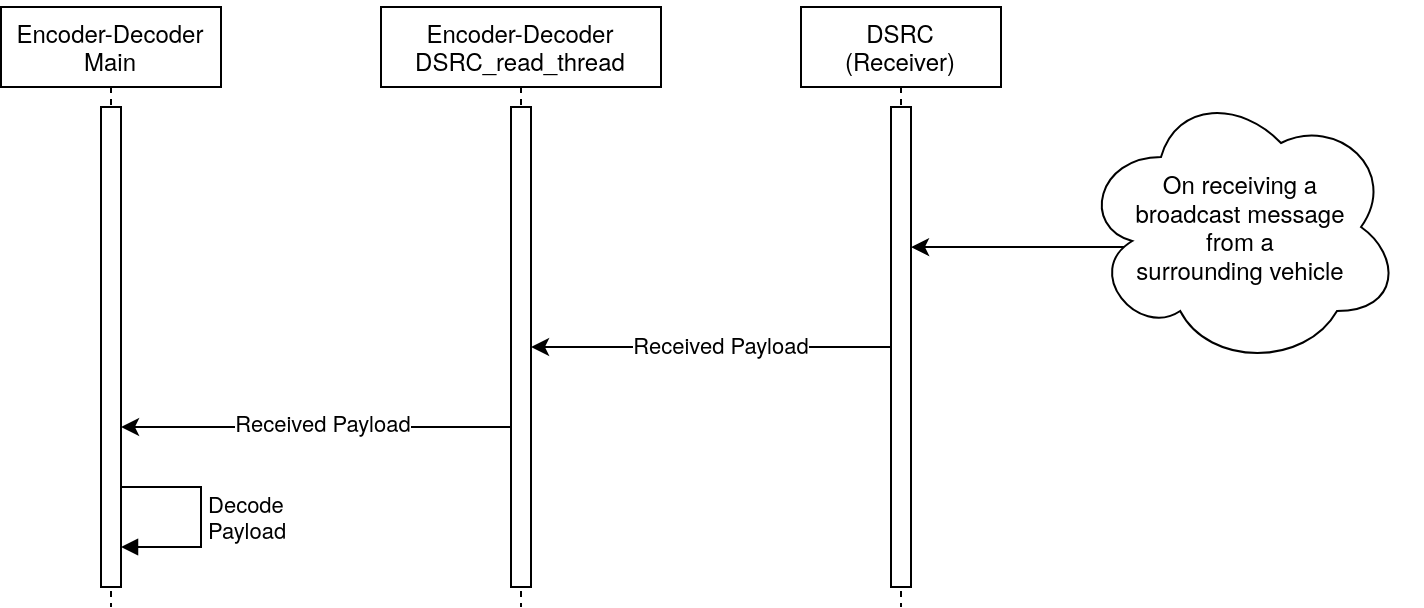
\includegraphics[scale=0.4]{Figures/ReceptionandBroadcast.png}
\caption[DSRC Reception and Broadcast]{DSRC Reception and Broadcast}
\label{fig:DSRC Reception and Broadcast1}
\end{figure}

\clearpage

\begin{figure}[!ht]
\centering
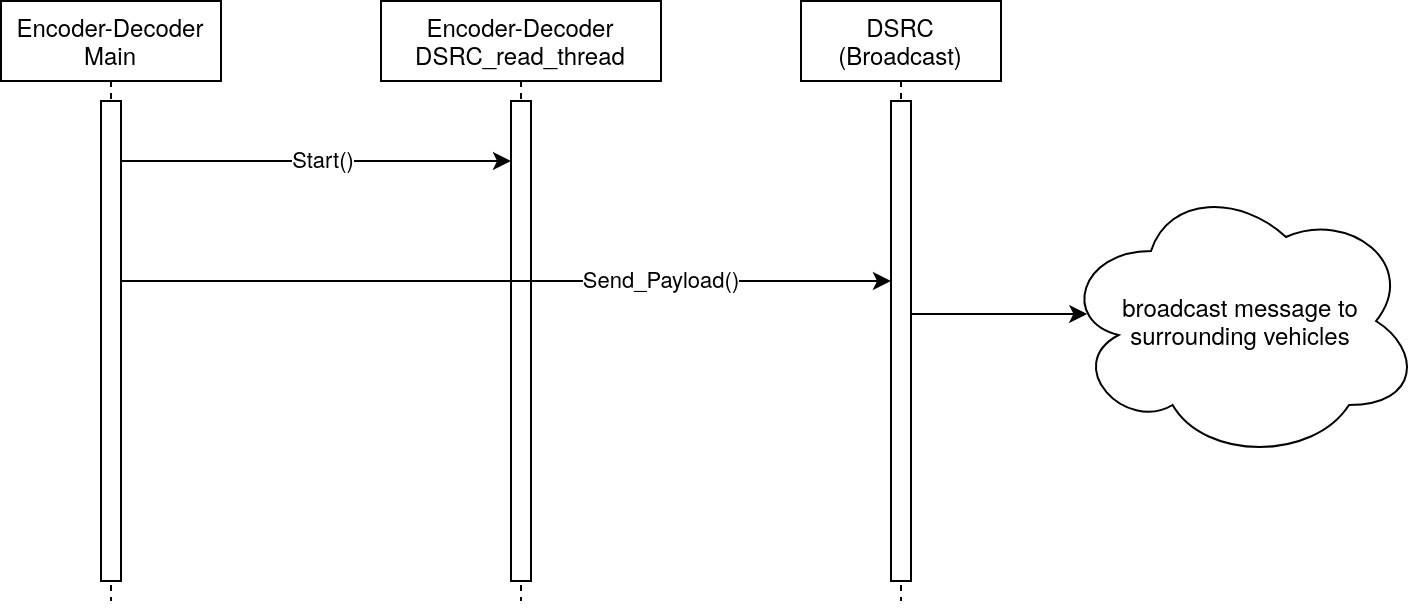
\includegraphics[scale=0.4]{Figures/ReceptionandBroadcast(2).png}
\caption[ReceptionandBroadcast]{DSRC Reception and Broadcast}
\label{fig:DSRC Reception and Broadcast2}
\end{figure}



Upon receiving the payload message from the Encoder/Decoder via UART, the DSRC module plays a vital role in broadcasting the message to surrounding vehicles. Equipped with both a sender and a receiver, all vehicles within the network are capable of communicating via DSRC. The DSRC module decodes the received payload message, independently extracting the ID byte to determine the payload type and identify the appropriate payload stack for storage.

\begin{figure}[!ht]
\centering
\includegraphics[scale=0.4]{31.png}
\caption[EncoderDecoder generate payload and send on an ESP and receive payload and decode on another]{Encoder/Decoder generate payload and send on an ESP and receive payload and decode on another}
\label{fig:TCU}
\end{figure}
\begin{figure}[!ht]
\centering
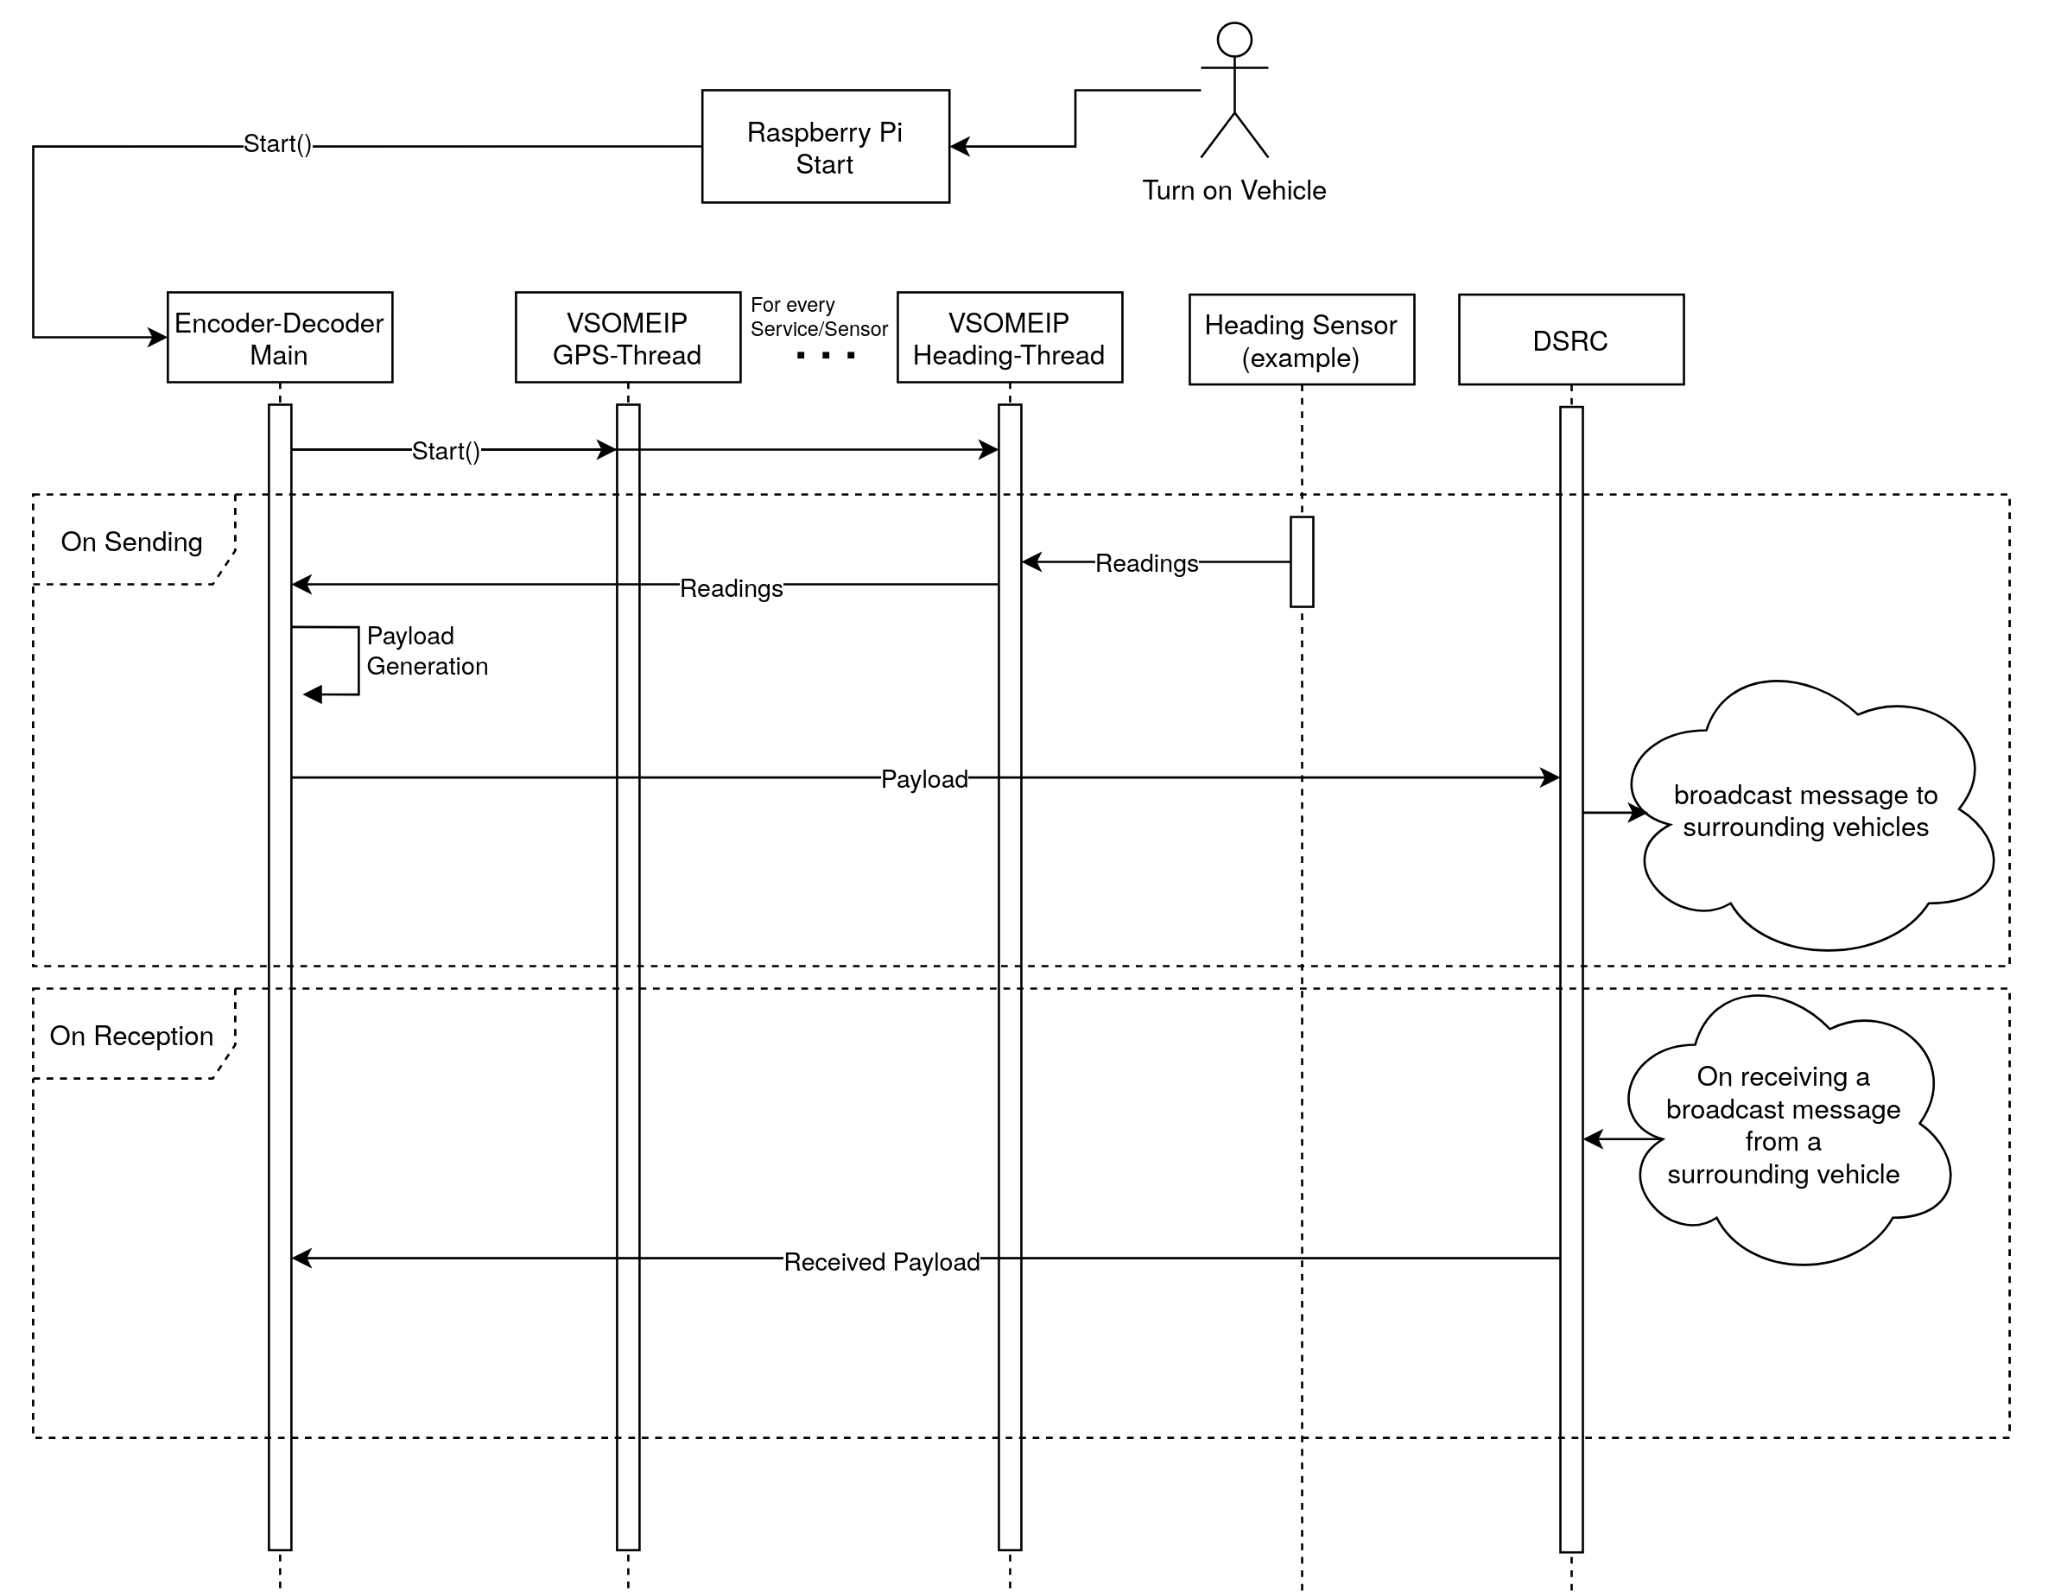
\includegraphics[scale=0.2]{32.png}
\caption[Encoder/Decoder operation UML sequence diagram]{Encoder/Decoder operation UML sequence diagram}
\label{fig:TCU}
\end{figure}
\chapter{TCU Simulation}
\section{Introduction}
In the context of understanding and visualizing the essential processes of a car, as well as its interactions with surrounding vehicles, we have developed a Unity simulation for a V2V (Vehicle-to-Vehicle) graduation project. This simulation serves as a virtual environment that accurately replicates real-world scenarios, enabling us to study and analyse the behaviour of vehicles and their communication protocols. The simulation incorporates the Encoder/Decoder module, which emulates the functionalities of a real vehicle, allowing for realistic interactions with the surrounding virtual vehicles.

\section{The Purpose of the Simulation}
The primary objective of our Unity simulation is to provide a comprehensive visualization of a car's operations and its communication with other vehicles. By creating a virtual representation of a car, we aim to study various aspects such as vehicle behaviour, sensor data capture, communication protocols, and the impact of V2V interactions. The simulation offers a unique opportunity to observe and analyse the intricate processes involved in V2V communication, thus contributing to the development of safer and more efficient transportation systems.
\begin{figure}[!ht]
\centering
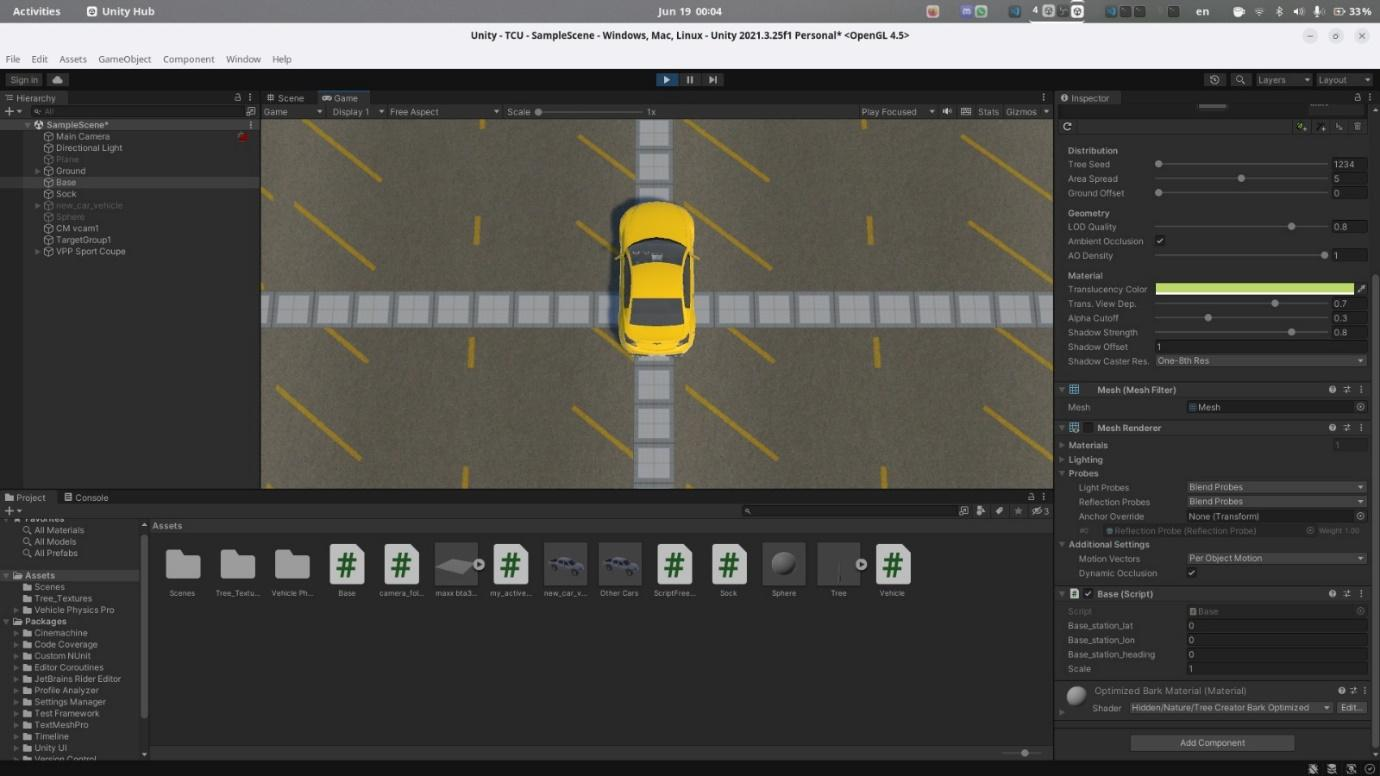
\includegraphics[scale=0.3]{33.png}
\caption[Simulation]{}
\label{fig:TCU}
\end{figure}
\section{Overview of the Encoder/Decoder in the Simulation}
Within the Unity simulation, the Encoder/Decoder module acts as a fundamental component, mirroring the functionalities of a real vehicle's Encoder/Decoder system. This software module is responsible for managing the communication between the virtual car and the real vehicles visible in the simulated environment. By emulating the behavior of a physical vehicle, we can accurately simulate the transmission and reception of payload messages, capturing sensor data, and interacting between the virtual and the real V2V network.

\section{Communication Architecture in the Simulation}
The communication architecture of the Unity simulation closely resembles the real-world V2V communication infrastructure. The Encoder/Decoder within the virtual car is designed to communicate with the DSRC (Dedicated Short-Range Communications) module, replicating the wireless broadcasting and receiving of payload messages. This architecture ensures that the virtual car can effectively exchange information with surrounding virtual vehicles, mimicking real V2V interactions.

\section{Sensor Data Capture and Processing}
The Unity simulation doesn't have real sensors because it is in a virtualized environment. However, it mimics the real-world data by calculating its distance from the Base station in the virtualized environment and calculated the supposed real-life GPS location given the Base station real GPS and the unity position and the virtual vehicle position in unity (by adjusting a scaling factor). This data is then passed to the Encoder/Decoder module, which processes and organizes it within a payload struct suitable for this information. The struct includes variables for storing sensor readings and a nested struct for capturing timestamps. This approach ensures the integrity and accessibility of the captured data for subsequent analysis and processing.

\section{Payload Generation and Broadcasting}
The Encoder/Decoder software is responsible for generating compact payloads that encapsulate any of our vehicles. However, when connected to any real vehicle, The readings come from real sensors through services concerned with fetching data from sensors and sent over VSOMEIP to the Encoder/Decoder. However, for unity simulation, there are no real sensors. So, simulated vehicle information is being sent to the Encoder/Decoder over Unix Sockets. The payloads are created as normal by the Encoder/Decoder module and are then sent to the surrounding vehicles as normal.

\section{DSRC Module: Reception and Broadcast}
Upon receiving the payload messages from neighboring virtual vehicles, the DSRC \cite{kenney2011dedicated} module receives the message, sends it to the Encoder/Decoder of the Unity simulation device, Encodes the message in a defined string format, and sends it over Unix socket to the Unity simulation. The Unity simulation decodes the messages, independently extracting the payload ID byte. This ID byte determines the type of payload received, allowing the simulation to identify the appropriate payload struct for storing the information. By simulating the DSRC module's reception and broadcasting capabilities, the simulation accurately replicates the behavior of a real V2V network.

\section{Memory Management and Struct Allocation}
When the DSRC module forwards received payload messages to the Encoder/Decoder within the simulation, the struct allocation process occurs. If no struct has been allocated for a specific virtual vehicle, the Encoder/Decoder module dynamically creates a new struct. This allocation ensures efficient organization and storage of sensor data, enabling subsequent direct access for detailed analysis and further processing.

\section{Data Analysis and Visualization}
With direct access to the virtual payload struct, the Unity simulation allows for in-depth data analysis and visualization. The simulation can also help retrieve the surrounding sensor's data, examine the timestamps, and perform various analytical operations to gain insights into vehicle behavior, V2V interactions, and system performance. The simulation provides a powerful platform for assessing the effectiveness of V2V protocols and developing advanced algorithms for enhanced safety and efficiency.

\clearpage
\begin{figure}[!ht]
\centering
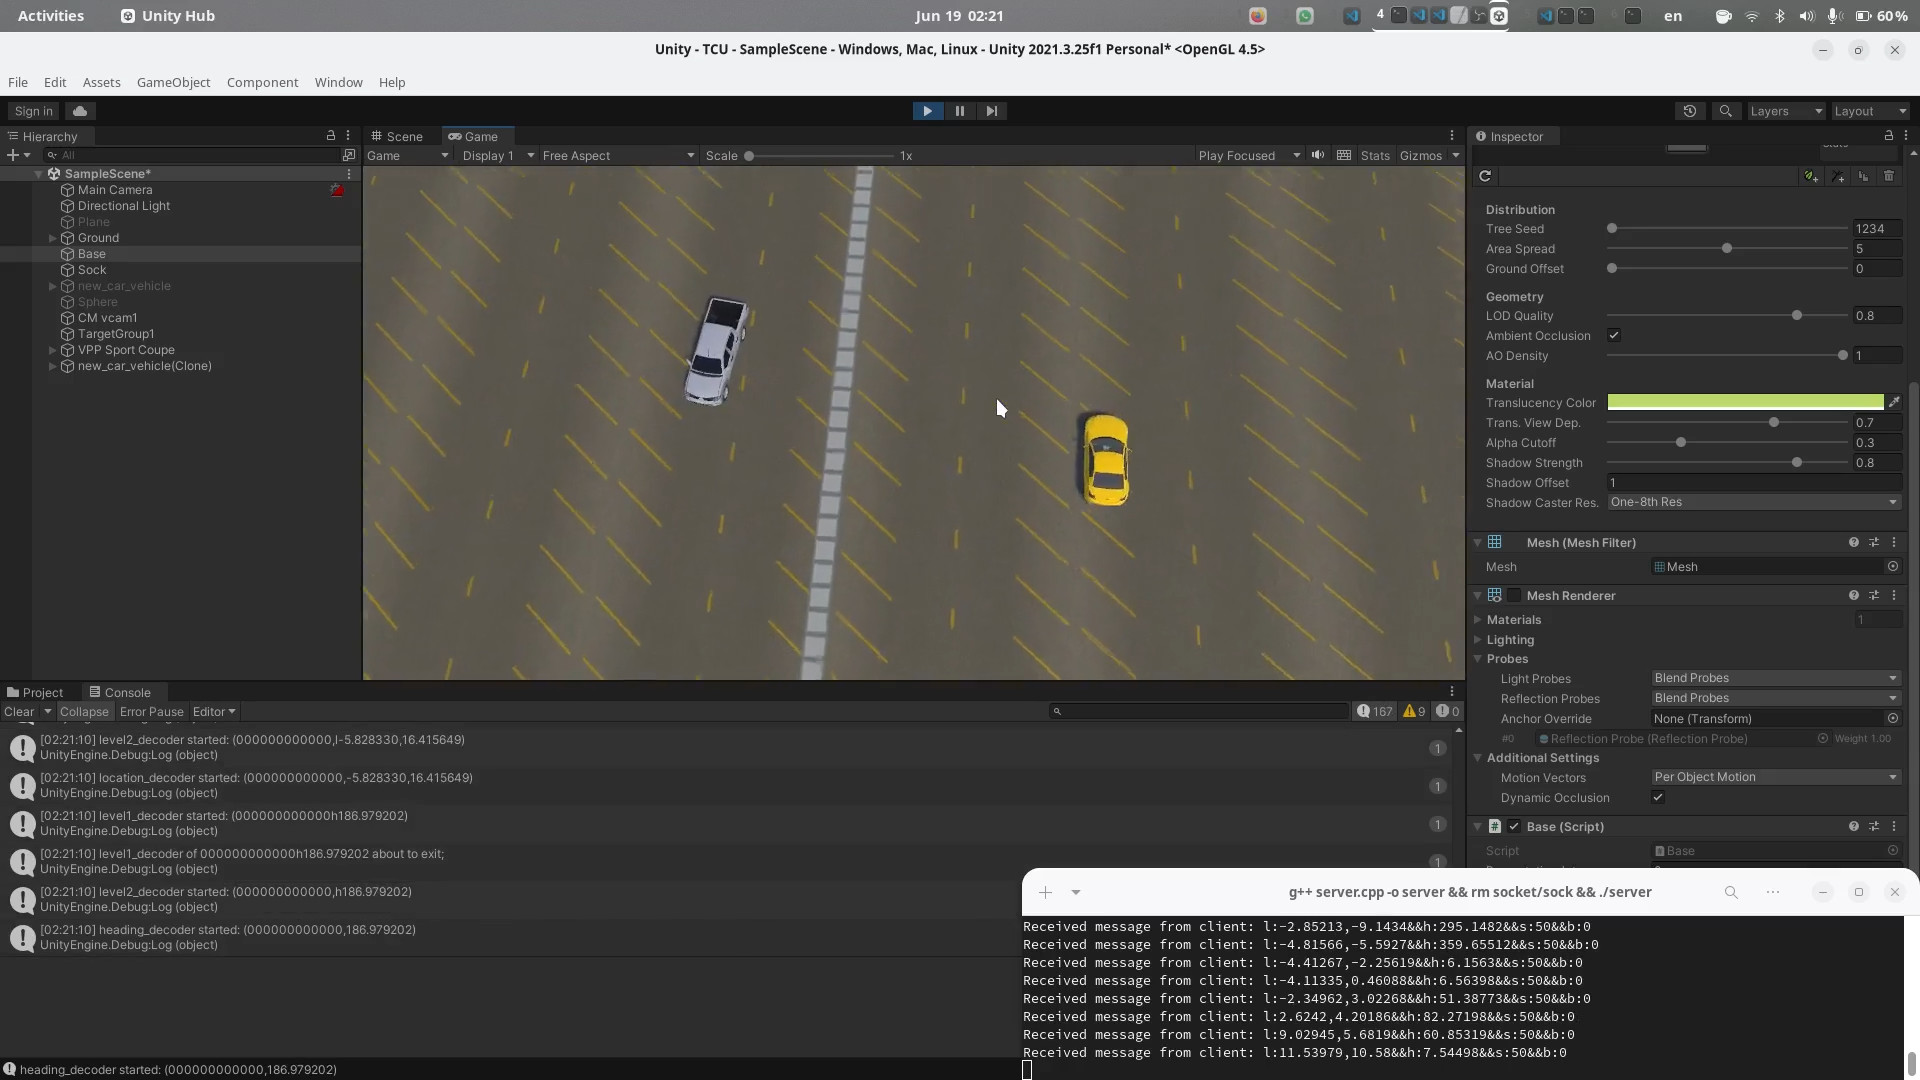
\includegraphics[scale=0.2]{34.png}
\caption[Simulation]{Simulation on Unity}
\label{fig:Simulation}
\end{figure}
\section{Conclusion}
The Unity simulation presented in this documentation offers a valuable tool for studying V2V communication, visualizing vehicle processes, and analyzing sensor data within a controlled virtual environment. By incorporating an Encoder/Decoder module, the simulation emulates the behavior of a real vehicle, enabling realistic interactions with surrounding virtual vehicles. This comprehensive and dynamic simulation framework contributes to the advancement of V2V technologies, ultimately leading to safer and more intelligent transportation systems.
\chapter{External ECUs}
\section{Overview of the External ECUs}
In an interconnected system where multiple Electronic Control Units (ECUs) collaborate, each ECU serves a specific purpose and contributes to the overall functionality and efficiency of the system. We have four main ECUs interconnected through Ethernet, each responsible for distinct tasks:
Speed ECU: The Speed ECU plays a vital role in monitoring and measuring the speed of the system. This information is crucial for numerous applications, including navigation systems, adaptive cruise control, and speed-dependent operations.
Heading ECU: The Heading ECU focuses on providing heading or directional information. It employs sensor magnetometers to detect the orientation or heading of the system with respect to a specific reference point, such as true north.
Diagnostic ECU: The Diagnostic ECU offers comprehensive fault diagnostic information pertaining to various aspects of the vehicle, including but not limited to tire pressure, battery health, and headlight functionality. the Diagnostic ECU can identify and report any abnormalities or issues, aiding in proactive maintenance, fault detection, and system health management.
MQTT ECU: The MQTT (Message Queuing Telemetry Transport) ECU serves as a bridge between the ECUs and the Transmission Control Unit (TCU). Its primary function is to wake up the TCU and facilitate communication between the TCU and other ECUs. The MQTT ECU uses the MQTT protocol to establish a connection, exchange messages, and retrieve relevant information from the TCU. This enables the ECUs to access real-time data from the TCU, enabling seamless integration and coordination between various components of the system.
By integrating these ECUs through an Ethernet connection, a robust and interconnected system is established. The Ethernet network allows for efficient and reliable communication among the ECUs, facilitating the exchange of data, control signals, and status updates. This connectivity enables the system to operate harmoniously, with each ECU contributing its specialized functionality to ensure accurate speed monitoring, precise heading information, comprehensive diagnostics, and seamless interaction with the TCU.
Moreover, this interconnected system offers flexibility and scalability, allowing for the addition of more ECUs or the integration of new functionalities as the requirements evolve. 
\section{Hardware Components of External ECUs}
\subsection{STM32}
\subsubsection{What is STM32?}
STM32 refers to a family of microcontrollers manufactured by STMicroelectronics. The STM32 microcontrollers are based on the ARM Cortex-M processor cores and are widely used in a variety of embedded systems and applications.

The STM32 family offers a wide range of microcontroller options, including different series and variants, to cater to different requirements and use cases. These microcontrollers are designed to provide a balance between performance, power efficiency, and cost-effectiveness.

The STM32 microcontrollers are known for their extensive feature sets, which typically include features such as multiple I/O ports, timers, communication interfaces (such as UART, SPI, I2C), analog-to-digital converters (ADCs), digital-to-analog converters (DACs), and various other peripherals.

The STM32 microcontrollers find applications in a wide range of industries, including automotive, industrial automation, consumer electronics, healthcare, and Internet of Things (IoT). They are often used in applications such as motor control, sensor interfacing, data acquisition, human-machine interfaces, communication devices, and more.
\begin{figure}[!ht]
\centering
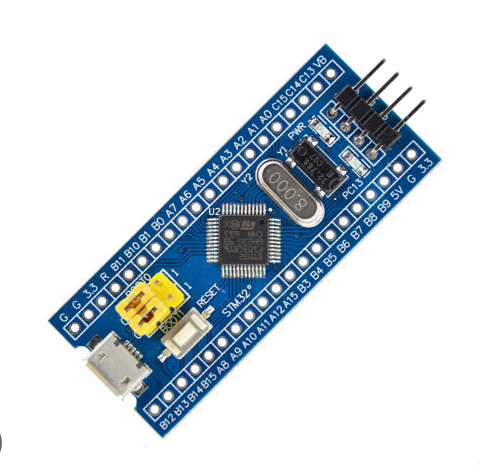
\includegraphics[scale=0.3]{STM32.png}
\caption[STM32]{STM32 MCU}
\label{fig:TCU}
\end{figure}
\subsubsection{STM32 Specifications}
\begin{itemize}
    \item Core Architecture: ARM Cortex-M3
    \item Clock Speed: Up to 72 MHz
    \item Flash Memory: 64 KB
    \item RAM: 20 KB
    \item 37 General-purpose I/O (GPIO) pins
    \begin{itemize}
        \item USART/UART (Universal Synchronous/Asynchronous Receiver/Transmitter)
        \item SPI (Serial Peripheral Interface)
        \item I2C (Inter-Integrated Circuit)
        \item USB (Universal Serial Bus)
        \item CAN (Controller Area Network)
        \item ADC (Analog-to-Digital Converter) with up to 16 channels
        \item DAC (Digital-to-Analog Converter) with 2 channels
        \item Timers: 3 General Purpose Timers, 2 Advanced Control Timers, 1 Basic Timer
        \item Real-Time Clock (RTC)
        \item Watchdog Timer
        \item DMA (Direct Memory Access) controller
        \item PWM (Pulse-Width Modulation) outputs
        \item External Interrupts
    \end{itemize}
    \item Operating Voltage Range: 2.0V to 3.6V
    \item Operating Temperature Range: -40°C to 85°C
    \item Power Consumption: Varies based on the operating mode (active, sleep, low-power modes, etc.) and the specific usage scenario.
    \item Package Type: LQFP (Low-Profile Quad Flat Package)
    \item Package Pin Count: 48 pins
\end{itemize}

\subsection{W5500}
\subsubsection{What is W5500}
The W5500 is a popular Ethernet controller chip designed for embedded systems and Internet of Things (IoT) applications. It is developed by WIZnet, a leading provider of Internet connectivity solutions.
The W5500 chip integrates a full hardware TCP/IP stack, allowing devices to establish and manage Ethernet connections with ease. It supports the standard Ethernet communication protocols such as TCP, UDP, IPv4, ICMP, ARP, and IGMP. This makes it suitable for applications that require reliable and efficient networking capabilities.
\subsubsection{W5500 Specifications}
\begin{figure}[!ht]
\centering
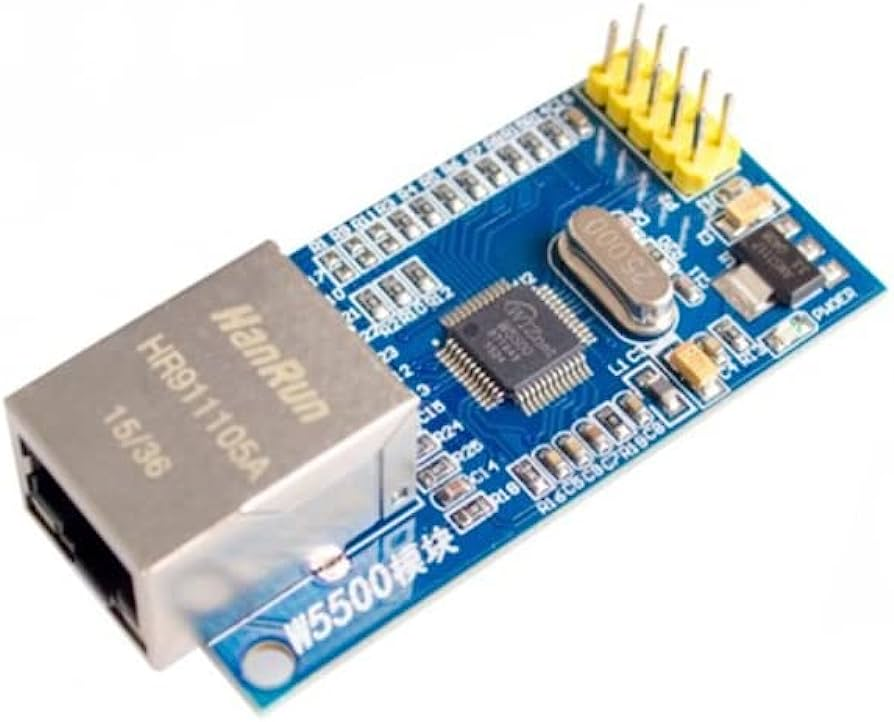
\includegraphics[scale=0.1]{W5500.png}
\caption[W5500]{W5500 module}
\label{fig:TCU}
\end{figure}
\begin{itemize}
\item Ethernet Interface: The chip provides a standard Ethernet interface with 10/100Mbps speed. It supports both full-duplex and half-duplex communication modes.
\item TCP/IP Stack: The W5500 incorporates a complete TCP/IP protocol stack in hardware, offloading the network processing tasks from the microcontroller or host processor. This relieves the burden on the main system and improves performance.
\item Hardware TCP/IP Processing: The chip handles various network functions, such as socket management, packet handling, IP fragmentation, retransmission, and checksum calculation, in hardware. This results in faster and more efficient network communication.
\item SPI Interface: The W5500 is typically interfaced with a microcontroller or host processor using the Serial Peripheral Interface (SPI). It communicates with the host system through SPI commands and data transfers.
\item Multiple Socket Support: The W5500 supports multiple simultaneous socket connections, allowing the device to handle multiple network connections concurrently. This is particularly useful for applications requiring multiple client-server connections or simultaneous data transfers.
\item Built-in Memory: The chip includes built-in memory for data buffering and storing network-related information, such as socket status, transmit/receive buffers, and socket options.
\item Low Power Consumption: The W5500 is designed to minimize power consumption, making it suitable for energy-efficient applications and battery-powered devices.
\item Support for Various Protocols: In addition to TCP/IP, the W5500 also supports other network protocols like UDP, IPv4, ICMP, ARP, and IGMP. This enables a wide range of network communication possibilities.
\end{itemize}
\subsection{4G Modem and Router}
\subsubsection{What is 4G Modem and Router?}
A 4G modem and router is a networking device that combines the functionalities of a 4G modem and a router in a single device. It enables users to connect to the internet using a 4G mobile broadband network and provides local network connectivity for multiple devices through wired or wireless connections. In the context of our project, we will utilize the 4G modem and router to establish an internet connection for our vehicle, ensuring reliable and high-speed internet access.
\begin{figure}[!ht]
\centering
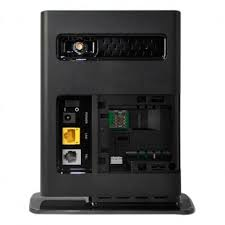
\includegraphics[scale=0.4]{4G Modem.png}
\caption[4G Modem Router]{4G Modem Router}
\label{fig:TCU}
\end{figure}
\subsubsection{Specifications}
\begin{itemize}
    \item Network Connectivity:
    \begin{enumerate}
        \item 4G LTE: Supports LTE Category 4 technology, offering download speeds of up to 150Mbps and upload speeds of up to 50Mbps.
        \item 3G: Provides fallback support for 3G networks (UMTS/HSPA) with download speeds of up to 42Mbps and upload speeds of up to 5.76Mbps.
        \item 2G: Supports GSM/GPRS/EDGE networks for basic cellular connectivity.
    \end{enumerate}
    \item Wireless Standards and Bands:
    \begin{enumerate}
        \item Wi-Fi: Supports 802.11b/g/n wireless standards, allowing for compatibility with a wide range of devices.
        \item Dual-Band: Operates on both 2.4GHz and 5GHz frequencies, providing flexibility and minimizing interference.
        \item Multiple Input Multiple Output (MIMO): Utilizes MIMO technology for improved wireless performance and coverage.
    \end{enumerate}
    \item Ethernet Ports:
    \begin{enumerate}
        \item LAN Ports: Equipped with four Ethernet LAN ports to establish wired connections with devices such as computers, gaming consoles, and smart TVs.
        \item WAN Port: Features one Ethernet WAN port for connecting to an external internet source or another router for additional network expansion.
    \end{enumerate}
    \item Voice Features:
    \begin{enumerate}
        \item Voice over IP (VoIP): Supports VoIP functionality for making and receiving phone calls over the internet.
        \item RJ11 Port: Includes an RJ11 port for connecting a telephone handset or fax machine.
    \end{enumerate}
    \item SIM Card Slot:
    \begin{enumerate}
        \item Supports a standard-sized SIM card for accessing the 4G LTE network and establishing internet connectivity.
    \end{enumerate}
    \item External Antenna Ports:
    \begin{enumerate}
        \item Provides two external antenna ports for connecting external antennas to enhance signal reception and coverage in areas with weak network signals.
    \end{enumerate}
    \item Security Features:
    \begin{enumerate}
        \item Built-in Firewall: Includes a built-in firewall for network security and protection against unauthorized access.
        \item WPA/WPA2 Encryption: Supports wireless encryption protocols (WPA and WPA2) to secure the wireless network.
    \end{enumerate}
    \item Management and Configuration:
    \begin{enumerate}
        \item Web Interface: Allows users to access and configure router settings through a web-based management interface.
        \item Mobile App: Offers a mobile app for easy management and monitoring of the router using a smartphone or tablet.
    \end{enumerate}
    \item Design and Dimensions:
    \begin{enumerate}
        \item Compact Design: Features a compact and sleek design suitable for home and small office environments.
        \item Dimensions: Typically measures around 190mm x 35mm x 176mm (W x H x D).
    \end{enumerate}
\end{itemize}
\subsection{Ethernet Switch}
\subsubsection{What is an Ethernet Switch?}
An Ethernet switch is a networking device that facilitates the efficient and reliable communication between multiple devices within a local area network (LAN). It serves as a central point for connecting and managing network devices, such as computers, servers, printers, and other Ethernet-enabled devices.
\begin{figure}[!ht]
\centering
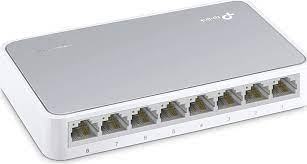
\includegraphics[scale=0.4]{Switch.png}
\caption[Switch]{Ethernet Switch}
\label{fig:TCU}
\end{figure}
\subsubsection{Switch Specifications}
\begin{itemize}
    \item \textbf{Network Segmentation}: An Ethernet switch enables the division of a LAN into multiple segments or network segments. Each port on the switch serves as an individual connection point for a device, allowing data to be sent and received within the specific segment it is connected to. This segmentation helps in improving network performance and reducing network congestion.
    \item \textbf{Packet Switching}: When data is transmitted from one device to another within the network, an Ethernet switch uses packet switching to efficiently route the data packets to the appropriate destination. The switch examines the destination MAC address of each incoming packet and forwards it only to the specific port where the destination device is connected, optimizing network traffic and minimizing data collisions.
    \item \textbf{MAC Address Learning}: Ethernet switches have the ability to learn and store the MAC addresses of devices connected to each of its ports. This information is stored in a table called the MAC address table or forwarding table. By maintaining this table, the switch can make forwarding decisions based on MAC addresses, ensuring that data is directed only to the intended recipients.
    \item \textbf{Full Duplex Communication}: An Ethernet switch supports full-duplex communication, allowing devices to transmit and receive data simultaneously at their maximum network speed. This feature enables faster and more efficient data transfer within the network.
    \item \textbf{Port Speed and Auto-negotiation}: Ethernet switches offer different port speeds, commonly 10/100/1000 Mbps (megabits per second) or Gigabit Ethernet. These speeds determine the maximum data transfer rate supported by each port. Additionally, switches support auto-negotiation, which allows the switch and connected devices to automatically determine and set the best available speed and communication mode.
\end{itemize}
\subsection{Hall Effect Sensor}

\subsubsection{What is Hall Effect Sensor?}
A Hall effect sensor is a transducer that detects the presence of a magnetic field and converts it into an electrical signal. Hall effect sensors are commonly used in various applications for their ability to measure magnetic fields accurately and provide real-time feedback.

The working principle of a Hall effect sensor is based on the Hall effect, which states that when a current-carrying conductor is exposed to a perpendicular magnetic field, a voltage difference is induced across the conductor. This voltage, known as the Hall voltage, is directly proportional to the strength of the magnetic field.

A Hall effect sensor typically consists of a thin strip or a semiconductor material, often made of gallium arsenide or indium antimonide. The strip carries a current and is placed perpendicular to the magnetic field being measured. When a magnetic field is applied, it causes electrons within the strip to be deflected to one side, creating an imbalance of charges. This charge imbalance generates the Hall voltage across the sensor.

The Hall voltage is then amplified and processed by electronic circuitry within the sensor, producing a usable output signal. The output can be analog (proportional voltage or current) or digital (on/off signal) depending on the sensor's design and application requirements.


\begin{figure}[!ht]
\centering
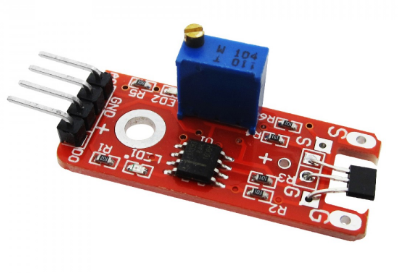
\includegraphics[scale=0.4]{HALL EFFECT SENSOR.png}
\caption[HALL EFFECT SENSOR]{Hall effect sensor module}
\label{fig:TCU}
\end{figure}

\subsubsection{Hall Effect Sensor Specifications}
\begin{itemize}
\item Operating Voltage: 5V DC
\item Output Voltage: Analog output
\item Detection Range: ±10 Gauss
\item Sensitivity: Approximately 2.5mV/Gauss
\item Operating Temperature: -40°C to +85°C
\item Dimensions: Approximately 29mm x 16mm x 13mm (L x W x H)
\item Weight: Approximately 3 grams
\item Mounting: The module usually comes with pre-drilled holes for easy installation and mounting on a circuit board or project enclosure.
\end{itemize}
\subsection{MPU6050}

\subsubsection{What is MPU6050?}

The MPU6050 with Magnetometer, also known as MPU6050+HMC5883L, is an enhanced version of the MPU6050 motion tracking device that incorporates an additional magnetometer or digital compass. This combination allows for comprehensive motion sensing and orientation tracking by integrating a three-axis accelerometer, a three-axis gyroscope, and a three-axis magnetometer within a single module.

\begin{figure}[!ht]
\centering
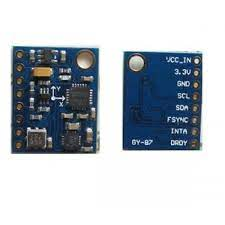
\includegraphics[scale=0.5]{mpu6050.png}
\caption[mpu6050]{MPU 6050 Module}
\label{fig:MPU6050}
\end{figure}

\subsubsection{MPU6050 Specifications}
\begin{itemize}
\item Accelerometer: The integrated three-axis accelerometer measures linear acceleration in three perpendicular directions (X, Y, and Z axes). It provides accurate data on changes in velocity and enables motion detection and vibration monitoring.
\item Gyroscope: The module features a three-axis gyroscope that measures angular velocity and rotation around the X, Y, and Z axes. It facilitates precise tracking of rotational movements and orientation changes.
\item Magnetometer (Digital Compass): The addition of a three-axis magnetometer allows for the measurement of the surrounding magnetic field. This enables orientation estimation with respect to Earth's magnetic field and provides compass functionality.
\item Digital Motion Processor (DMP): The MPU6050 with Magnetometer integrates a Digital Motion Processor, which offloads sensor fusion and sensor data processing tasks from the primary microcontroller or processor. The DMP combines data from the accelerometer, gyroscope, and magnetometer to provide fused and calibrated motion tracking outputs.
\item I2C Interface: Similar to the original MPU6050, the module communicates with the host microcontroller or processor using the widely-used I2C (Inter-Integrated Circuit) protocol, simplifying interfacing with various microcontrollers.
\item Motion Processing Capabilities: The enhanced module retains the advanced motion processing features of the MPU6050, including programmable digital filters, gesture recognition, and motion detection interrupt functionality. These features enable applications such as gaming, robotics, motion-controlled user interfaces, and inertial navigation systems.
\item Low Power Consumption: The module maintains the low power consumption characteristics of the MPU6050, making it suitable for energy-efficient and battery-powered devices.
\item Temperature Sensor: The MPU6050 with Magnetometer integrates an embedded temperature sensor, allowing accurate temperature measurements to account for environmental temperature changes that may affect the performance or calibration of the sensor outputs.
\end{itemize}

\subsection{Vibration and Shock Sensor}

\subsubsection{What is Vibration and Shock Sensor?}

The vibration sensor is a highly sensitive device employed for detecting and monitoring impact forces, shocks, and vibrations. Its main purpose is to accurately sense and analyze mechanical disturbances while effectively suppressing background noise that may interfere with the reliability of vibration measurements.

Comprising essential components such as a piezoelectric element, spring oscillator, sensitivity adjustment knob, and LED indicator, the vibration sensor is designed for optimal performance. The piezoelectric element plays a crucial role in converting mechanical vibrations into electrical signals, enabling precise detection and measurement of the impact forces and vibrations.

The spring oscillator mechanism ensures the sensor's responsiveness to varying levels of impact and vibration. By adjusting the sensitivity adjustment knob, users can fine-tune the sensor's sensitivity to suit specific requirements. For instance, rotating the knob clockwise enhances the sensor's sensitivity, allowing it to detect even subtle vibrations, while the LED indicator provides a visual cue by lighting up when the sensor registers impacts within a certain range.

This adjustable sensitivity feature of the vibration sensor enables customization to the desired level of responsiveness, making it versatile and adaptable for different applications. It ensures optimal performance by minimizing false readings caused by extraneous vibrations or background noise.
\begin{figure}[!ht]
\centering
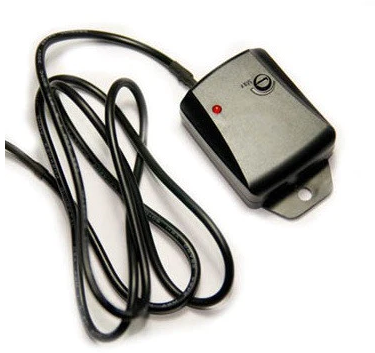
\includegraphics[scale=0.2]{VibrationANDShockSensor.png}
\caption[VibrationANDShockSensor]{Vibration sensing sensor}
\label{fig:TCU}
\end{figure}

\textbf{Vibration and Shock Sensor Specifications}
\begin{itemize}
\item Power requirements: DC 12V
\item Operating Temperature: $-30^\circ$C to $65^\circ$C
\item Dimensions: 45mm $\times$ 38mm $\times$ 20mm
\end{itemize}

\chapter{Software Hardware Interfacing and Connection}
\section{W5500 Interfacing with STM32}
\subsection{Introduction}
One of the notable limitations of STM32 microcontrollers is the absence of built-in Ethernet functionality. Unlike some other microcontrollers or systems-on-chip (SoCs) that come with integrated Ethernet controllers, STM32 microcontrollers primarily focus on providing a rich set of general-purpose input/output (GPIO) pins, a high-performance core, and various peripherals for different application needs. Ethernet connectivity, however, is not among these built-in features.

To overcome this limitation, we can turn to external modules that provide Ethernet connectivity. The W5500 module, specifically designed for SPI-to-Ethernet communication, acts as an intermediary between the STM32 microcontroller and the Ethernet network. It serves as an Ethernet controller that handles the complexities of Ethernet communication, allowing the STM32 microcontroller to seamlessly connect to Ethernet networks.

By integrating the W5500 module with an STM32 microcontroller, we gain the ability to establish bidirectional communication with Ethernet networks. The module takes care of the low-level Ethernet protocols, including packet formatting, transmission, and reception, while the STM32 microcontroller focuses on higher-level application tasks.

The W5500 module's SPI interface is well-suited for interfacing with STM32 microcontrollers. The SPI protocol is a widely used serial communication interface that allows efficient data transfer between the microcontroller and external devices. The STM32 microcontroller's SPI peripheral, combined with the SPI pins of the W5500 module, provides a reliable and straightforward means of communication between the two components.

Moreover, the W5500 module offers a range of features that make it an attractive choice for adding Ethernet connectivity to STM32 microcontroller projects. It incorporates a TCP/IP protocol stack directly on the module, eliminating the need for us to implement complex networking protocols from scratch. This integration simplifies the development process and accelerates time-to-market for Ethernet-enabled applications.

Furthermore, the W5500 module supports high-speed Ethernet communication, with capabilities of 10/100Mbps. This allows for fast and efficient data transfer between the STM32 microcontroller and the Ethernet network, enabling real-time communication, streaming applications, and quick response times for networked systems.

In addition, the W5500 module provides flexibility in network configuration. Developers can easily set up IP addresses, subnet masks, gateways, and MAC addresses to match the requirements of their specific applications and network environments. This configurability allows seamless integration with existing network infrastructures and ensures proper communication and data exchange within the network.

While STM32 microcontrollers lack built-in Ethernet functionality, the incorporation of the W5500 module presents an effective solution to this limitation. By integrating the W5500 module via the SPI interface, developers can empower their STM32 microcontroller projects with Ethernet connectivity, enabling seamless communication, data transfer, and interaction with Ethernet networks.

\subsection{Hardware Connection}

The Serial Peripheral Interface (SPI) is a widely used communication protocol for synchronous data transfer between a master device and one or more slave devices. In the case of the W5500 module and an STM32 microcontroller, the SPI protocol is employed to establish a reliable and efficient communication link.

The SPI connection between the W5500 module and the STM32 microcontroller involves several key pins and signals:
\begin{itemize}
\item SCK (Serial Clock): This is the clock signal generated by the master device, which in this case is the STM32 microcontroller. The SCK pin of the STM32 microcontroller is connected to the SCK pin of the W5500 module. The SCK signal synchronizes the data transfer between the microcontroller and the module, ensuring that both devices operate at the same clock rate.
\item MISO (Master In Slave Out): This pin is the data line for transferring data from the slave device, the W5500 module, to the master device, the STM32 microcontroller. The MISO pin of the W5500 module is connected to the MISO pin of the STM32 microcontroller. When the microcontroller sends a request or reads data from the module, the module responds by transmitting the requested data over the MISO line.
\item MOSI (Master Out Slave In): This pin is the data line for transferring data from the master device, the STM32 microcontroller, to the slave device, the W5500 module. The MOSI pin of the STM32 microcontroller is connected to the MOSI pin of the W5500 module. When the microcontroller needs to send data or commands to the module, it transmits them over the MOSI line.
\item CS (Chip Select): The Chip Select pin is used to select the specific slave device with which the master device wants to communicate. In this case, the CS pin of the W5500 module is connected to a GPIO pin of the STM32 microcontroller. By asserting the CS pin, the microcontroller activates the W5500 module and initiates communication with it.
\end{itemize}

The SPI connection allows full-duplex communication, meaning that data can be transmitted in both directions simultaneously. The microcontroller and the W5500 module can exchange data and commands efficiently, enabling seamless communication between the two devices.
\begin{figure}[!ht]
\centering
\includegraphics[scale=0.4]{35.png}
\caption[SPI to Ethernet connection]{SPI to Ethernet connection}
\label{fig:TCU}
\end{figure}
\subsection{SPI Operational Mode}
\subsubsection*{The W5500 module offers two distinct SPI operation modes:}
\begin{itemize}
\item \textbf{Variable Length Data Mode}: In the variable length data mode, the W5500 module supports variable-length data transmission over the SPI interface. This means that the module can handle data packets of different lengths during communication with the STM32 microcontroller. In this mode, the microcontroller sends a command to the W5500 module to initiate data transmission. The module responds by transmitting the requested data, which can be of variable length, back to the microcontroller over the SPI bus. This flexibility allows for efficient data transfer, as the module can dynamically adjust the length of the transmitted data based on the requirements of the application or network protocol being used. The variable length data mode is useful in scenarios where the size of the data being transmitted may vary, such as in applications involving variable-sized packets or when dealing with protocols that support variable-length payloads.
\item \textbf{Fixed Length Data Mode}: In the fixed length data mode, the W5500 module operates with a predetermined fixed length for data transmission over the SPI interface. In this mode, the module transmits and receives data packets of a specific, preconfigured length. When the STM32 microcontroller communicates with the W5500 module using the fixed length data mode, it sends a command along with the desired data length to the module. The module then transmits or receives the specified number of data bytes to or from the microcontroller. This fixed length operation ensures consistent and predictable data transfer, especially in applications or protocols that rely on fixed-size data packets.
\end{itemize}

We deliberately chose to utilize the variable length data mode for our application, primarily because of its exceptional capability to seamlessly handle varying data sizes. By selecting this mode, we can accommodate the dynamic nature of the data being transmitted, allowing for efficient and optimized communication regardless of the fluctuating lengths of the data packets involved. This versatility ensures that our system can adapt to diverse scenarios where the size of the transmitted data may differ, such as in sensor networks. Thus, the variable length data mode empowers us to achieve optimal data transfer rates while minimizing unnecessary overhead, making it the ideal choice for our specific requirements.

\begin{figure}[!ht]
\centering
\includegraphics[scale=0.7]{36.png}
\caption[Spi master slave configuration]{Spi master slave configuration}
\label{fig:TCU}
\end{figure}


The SPI frame in the W5500 module refers to the structure and format of the data exchanged between the module and the microcontroller during SPI communication. It defines how the data is organized, transmitted, and received over the SPI bus.

The SPI frame in the W5500 module consists of the following components:
\begin{itemize}
    \item \textbf{Control Bits}: These bits serve as the command signals that instruct the W5500 module on the type of SPI transaction being performed. They determine whether it is a read or write operation, control various communication settings, and provide mode selection options. By manipulating the control bits, the microcontroller can precisely define the nature of the SPI transaction, enabling efficient data transfer and module configuration.
    \item \textbf{Address}: The address field within the SPI frame specifies the memory location or register within the W5500 module that is being accessed. It acts as a reference point, allowing the module to identify the specific data location to read from or write to during the SPI transaction. The address field ensures accurate data retrieval and manipulation within the module's internal memory or registers, facilitating seamless interaction with the microcontroller.
    \item \textbf{Data}: The data field carries the actual payload being transmitted or received during the SPI transaction. It can include a wide range of information, such as configuration settings, command instructions, or the actual data being exchanged between the W5500 module and the microcontroller. The data field enables the transfer of critical information, facilitating data processing, protocol implementation, and seamless integration with other system components.
\end{itemize}

The SPI frame format is typically determined by the protocol and specifications of the device, in this case, the W5500 module. It is important to adhere to the defined SPI frame structure to ensure proper communication and accurate data transfer between the module and the microcontroller.

During an SPI transaction, the microcontroller initiates the communication by sending the SPI frame with the appropriate control bits, address, and data to the W5500 module. The module then responds by transmitting the requested data back to the microcontroller, following the same frame format.
\begin{figure}[!ht]
\centering
\includegraphics[scale=0.5]{38.png}
\caption[SPI to Ethernet]{SPI to Ethernet}
\label{fig:SPI to Ethernet}
\end{figure}

\subsubsection{Initialization and Configuration}

We have utilized the Wizchip library to facilitate the implementation of UDP communication with the W5500 module. To establish communication between the STM32 microcontroller and the W5500 module, it is crucial to initialize the SPI communication and configure the W5500 module accordingly. This involves setting up the SPI peripheral of the microcontroller and configuring the necessary GPIO pins. Accurate configuration of SPI parameters such as clock frequency, data format, and SPI mode is important to match the requirements of the W5500 module.

Next, the W5500 module needs to be configured with the necessary network settings. This includes specifying the IP address, subnet mask, gateway address, and MAC address. These settings enable the module to communicate over the network and establish connections. By providing accurate network configurations, the module seamlessly integrates into the desired network environment.

In our case, we chose UDP (User Datagram Protocol) as the operating mode for communication. UDP is ideal for applications that require simple, connectionless communication, making it suitable for scenarios such as streaming sensor data. With UDP, time is critical as it allows for real-time data streaming without the overhead of establishing and maintaining connections.

To facilitate data transmission and reception, memory buffers are allocated within the W5500 module. These buffers serve as temporary storage areas for the data exchanged between the module and the microcontroller. The size of these buffers should be determined based on the specific requirements of the application, ensuring sufficient space for the expected data payload.

\textbf{Send Data}

To send data using UDP with the W5500 module, you can utilize the SPI interface of the STM32 microcontroller to communicate with the module. Here is a detailed explanation of the process:
\begin{enumerate}
    \item Set Destination IP Address and Port: Determine the destination IP address and port number to which you want to send the data. These parameters specify the network location of the receiving device or application. Assign the destination IP address and port number to appropriate variables or constants.
    \item Initialize UDP Socket: Initialize a UDP socket on the W5500 module. Configure the socket with the necessary parameters such as the source port number and protocol. The W5500 module provides registers to set up the socket, allowing you to define its behavior.
    \item Send UDP Packet: To send the UDP packet, you need to write the packet data to the W5500 module's internal TX buffer. Use the SPI interface of the STM32 microcontroller to communicate with the W5500 module. Send the SEND command to start transmitting.
\end{enumerate}

\textbf{Receive Data}

To receive data using UDP with the W5500 module, you can utilize the SPI interface of the STM32 microcontroller to communicate with the module. Here is a detailed explanation of the process:
\begin{enumerate}
    \item Initialize UDP Socket: Initialize a UDP socket on the W5500 module. Configure the socket with the necessary parameters such as the source port number and protocol. The W5500 module provides registers to set up the socket, allowing you to define its behavior.
    \item Send Receive Command: Once the module is ready to receive data, send the RECV command to the W5500 module to initiate the reception process. This command instructs the module to start listening for incoming UDP packets on the specified local port.
\end{enumerate}

\section{Hall Effect Sensor}
\begin{figure}[!ht]
\centering
\includegraphics[scale=0.5]{39.png}
\caption[Hall effect sensor module]{Hall effect sensor module}
\label{fig:TCU}
\end{figure}
\subsection{Introduction}
The measurement of vehicle speed is an essential aspect of automotive engineering. Accurate speed monitoring plays a critical role in numerous applications, such as ensuring road safety, optimizing fuel efficiency, implementing intelligent transportation systems, and enhancing driver assistance systems. Vehicle speed data is also valuable for navigation purposes, traffic management, and performance analysis in motorsports and automotive research.

We will focus on a specific method for speed measurement utilizing a Hall effect sensor. The Hall effect sensor is widely employed in various industries due to its reliability, simplicity, and cost-effectiveness. It operates based on the principle of the Hall effect, discovered by Edwin Hall in 1879. According to this principle, when a current-carrying conductor is exposed to a perpendicular magnetic field, a voltage difference is induced across the conductor. This effect forms the foundation for speed measurement in many applications, including automotive systems.

The utilization of a Hall effect sensor for speed measurement offers several advantages. Firstly, it provides a contactless method for obtaining speed information, eliminating the need for physical contact with the vehicle's moving components. This aspect enhances durability and reduces maintenance requirements. Secondly, Hall effect sensors are capable of detecting a wide range of speeds, making them suitable for both low-speed and high-speed applications. Additionally, Hall effect sensors exhibit excellent reliability and can operate in diverse environmental conditions, including extreme temperatures, moisture, and vibrations.

\subsection{Sensors for Speed Measurement}
\subsubsection{Why Hall Effect Sensor?}
There are several methods available for measuring vehicle speed, such as radar-based systems, wheel speed sensors, and GPS. In this project, a Hall effect sensor is employed due to its simplicity, reliability, and cost-effectiveness. The Hall effect sensor operates based on the principle of the Hall effect, which states that when a magnetic field is applied perpendicular to the direction of current flow in a conductor, a voltage difference is generated across the conductor. This effect is utilized in speed measurement by placing magnets on the rotating wheel and using the Hall effect sensor to detect the passage of these magnets.

\subsection{Pin Diagram of Hall Effect Sensor}
A Hall effect sensor consists of a semiconductor material with a current-carrying conductor placed within a magnetic field. When the magnetic field is perpendicular to the direction of the current flow, a voltage difference is generated across the conductor. This voltage, known as the Hall voltage, is directly proportional to the strength of the magnetic field and the current flowing through the conductor.

Hall effect sensors commonly used for speed measurement in automotive applications are typically integrated circuits (ICs) that contain the Hall effect sensor element along with signal conditioning circuitry. These ICs provide a convenient interface for connecting the sensor to a microcontroller or other electronic components.

The Hall effect sensor IC typically has three main pins:
\begin{itemize}
    \item Vcc (Power Supply): This pin is connected to the positive supply voltage, typically 5V or 3.3V, to power the sensor.
    \item GND (Ground): This pin is connected to the ground reference of the system.
    \item OUT (Output): This pin provides the output signal that corresponds to the detected magnetic field.
\end{itemize}

In speed measurement applications, the Hall effect sensor is positioned near a rotating component, such as a toothed wheel or gear, that contains one or more magnets. As the magnet passes by the Hall effect sensor, it generates a magnetic field that is detected by the sensor. This detection triggers an output signal change, allowing the measurement of the time interval between the passage of the magnets and subsequently calculating the speed based on the known distance between them.

In the following sections, we will delve into the details of the methodology, including sensor placement, hardware setup, software implementation, debouncing techniques, and the transmission of speed data to external devices. Through this comprehensive exploration, engineers and enthusiasts will gain valuable insights into utilizing Hall effect sensors for car speed measurement, enabling them to develop their speed monitoring systems with precision and reliability.

\subsection{Methodology: Utilizing the Hall Effect Sensor for Speed Calculation}
\begin{figure}[!ht]
\centering
\includegraphics[scale=0.2]{40.png}
\caption[Speed measuring using Hall effect sensor and magnet]{Speed measuring using Hall effect sensor and magnet}
\label{fig:TCU}
\end{figure}

The following steps outline the procedure for calculating car speed using a Hall effect sensor:

\subsubsection{Hardware Setup}
\begin{itemize}
    \item Mount the Hall effect sensor near the wheel or axle of the vehicle.
    \item Attach two magnets to the rotating wheel at a distance of 18.84 centimeters apart.
\end{itemize}

\subsubsection{Software Implementation}
\begin{itemize}
    \item Set up an interrupt routine to be triggered when the Hall effect sensor detects a passing magnet.
    \item Implement a timer to measure the time interval between the detection of two consecutive magnets.
    \item Calculate the speed using the formula: Speed = Distance / Time, where Distance is the known distance between the magnets and Time is the measured time interval.
\end{itemize}

\subsubsection{Debouncing}
\begin{itemize}
    \item To prevent erroneous readings caused by bouncing or multiple detections within a short period, implement a debouncing mechanism.
    \item Use a lock variable and timers to introduce a delay (e.g., 0.3 seconds) before accepting a new reading after the first detection.
\end{itemize}

\subsubsection{Speed Display}
\begin{itemize}
    \item Use another timer to trigger an interrupt at a set interval (e.g., every 1.1 seconds) to display the calculated speed.
    \item Format the speed information and transmit it via SPI or Ethernet to Raspberry Pi or other external devices.
\end{itemize}

\subsection{Conclusion}
In conclusion, we outlined a methodology for calculating car speed using a Hall effect sensor. By leveraging the magnetic field detection principle of the Hall effect, the sensor can accurately measure the time interval between the passage of two magnets attached to the rotating wheel of a car. This measured time interval allows for the calculation of the car's speed based on the known distance between the magnets.

The utilization of a Hall effect sensor offers several advantages for speed measurement in automotive applications. It provides a contactless method for obtaining speed information, enhancing durability and reducing maintenance requirements. Hall effect sensors are capable of detecting a wide range of speeds, making them suitable for various vehicle types and speed ranges. Additionally, Hall effect sensors exhibit excellent reliability and can operate in diverse environmental conditions, ensuring their usability in automotive applications.

The specific implementation of the methodology involves hardware setup, software implementation, debouncing techniques, and speed display. By following these steps, engineers and enthusiasts can develop their speed monitoring systems with precision and reliability. The calculated speed data can be displayed through UART or transmitted to external devices via communication interfaces such as SPI or Ethernet.

It is important to note that while this documentation provides a comprehensive overview of the methodology, additional considerations such as system calibration, error handling, and integration with specific vehicle and microcontroller platforms should be taken into account for accurate and reliable speed measurement.

By implementing this methodology, engineers and enthusiasts can derive valuable insights from vehicle speed data, contributing to the improvement of automotive systems, safety, and overall driving experience. The flexibility and cost-effectiveness of the Hall effect sensor make it a suitable choice for speed measurement in various automotive applications, enabling advancements in performance analysis, navigation, and intelligent transportation systems.

\section{Interfacing Compass Sensor}

\subsection{Introduction}
In order to provide accurate motion and direction detection, a variety of devices use the LSM6DSO compass sensor, an advanced electronic component. Its combination of a 3-axis accelerometer and a 3-axis magnetometer enables it to precisely monitor movement and calculate the orientation of the object with respect to the Earth's magnetic field. The components, operation, features, benefits, and drawbacks of the LSM6DSO compass sensor will all be covered in this thorough introduction.

The LSM6DSO compass sensor is made up of a number of vital parts that cooperate to deliver precise motion and direction information:

\begin{itemize}
  \item \textbf{3-Axis Accelerometer:} X, Y, and Z are three perpendicular axes that are measured by a 3-axis accelerometer, which measures linear acceleration along each of them. It enables the sensor to comprehend the movement of the gadget in three dimensions by detecting variations in velocity.
  \item \textbf{3-Axis Magnetometer:} The magnetometer gauges the strength and direction of the magnetic field that surrounds the sensor along the same three axes. The sensor can determine the orientation of the object in relation to the Earth's magnetic field by detecting it.
  \item \textbf{Control Interface:} The sensor has a control interface for connecting to a host device like a microcontroller or CPU and establishing communication with the LSM6DSO. I2C (Inter-Integrated Circuit) and SPI (Serial Peripheral Interface) are two common protocols used.
\end{itemize}

\subsection{How It's Done}
The LSM6DSO compass sensor functions as follows:

\begin{itemize}
  \item \textbf{Data from the 3-axis accelerometer:} This device measures the linear acceleration that the sensor experiences along each of its three axes (X, Y, and Z). The movement of the gadget is tracked using this data, and variations in velocity are calculated.
  \item \textbf{Data from the 3-axis magnetometer:} The magnetometer simultaneously measures the strength and direction of the magnetic field in the immediate vicinity along the same three axes. The Earth's magnetic field is particularly detected, serving as an orientation reference.
  \item \textbf{Sensor Fusion:} To determine the exact orientation of the device, the sensor fusion algorithm integrates information from the accelerometer and magnetometer. It establishes the device's heading (direction) and tilt angles by contrasting the detected magnetic field with the magnetic field of the known Earth.
  \item \textbf{Output:} By sending the calculated orientation data from the LSM6DSO sensor to the host device, applications can accurately track motion, ascertain orientation, and input data for augmented reality, virtual reality, navigation systems, and other related applications.
\end{itemize}

\subsection{Applications of Compass Sensor}
The compass sensor finds applications in various fields, including:

\begin{itemize}
  \item Motion tracking
  \item Virtual reality
  \item Wearable devices
  \item Fitness trackers
  \item Gesture recognition
  \item Gaming
  \item Industrial automation
  \item Robotics
\end{itemize}

\subsection{Features}
The LSM6DSO compass sensor has a number of noteworthy features that enhance its functionality and adaptability:

\begin{itemize}
  \item \textbf{High Accuracy:} The sensor delivers exact readings, ensuring accurate tracking of motion and orientation.
  \item \textbf{Low Power Consumption:} It is made to perform effectively while using the least amount of power possible, making it suited for battery-powered devices and extending the life of their batteries.
  \item \textbf{Compact Size:} The LSM6DSO sensor is small, which enables integration into a variety of electronic equipment without taking up much room.
  \item \textbf{Broad Measurement Range:} The sensor has a large measurement range for the magnetometer and accelerometer, allowing it to handle a variety of applications and environmental situations.
  \item \textbf{Integral Sensor Fusion:} The sensor has sensor fusion algorithms that integrate information from the magnetometer and accelerometer to provide trustworthy and precise orientation data.
\end{itemize}

\subsection{Advantages of Compass Sensor}
The LSM6DSO compass sensor offers several advantages.

\begin{itemize}
  \item \textbf{Small and low-power:} The LSM6DSO is a very small and low-power sensor, which makes it perfect for wearable technology and other applications where size and power consumption are important considerations.
  \item \textbf{High sampling rate:} The LSM6DSO has a high sampling rate of up to 1000 Hz, allowing it to record extremely minute motion details.
  \item \textbf{Wide temperature range:} With a temperature range of -40 to +85°C, the LSM6DSO is appropriate for usage in a variety of settings.
  \item \textbf{Built-in DMP:} The LSM6DSO comes equipped with a digital motion processor (DMP) that can handle challenging motion processing jobs. The host microcontroller may then have more time to work on other projects, such data logging or user interface.
  \item \textbf{I2C and SPI interfaces:} The LSM6DSO is offered in both I2C and SPI variants, making it compatible with a variety of microcontrollers.
  \item \textbf{Supported by a range of development tools:} The LSM6DSO is supported by a range of development tools, making it simple to get started with the sensor.
\end{itemize}

\subsection*{Drawbacks of Compass Sensor}
Despite its advantages, the LSM6DSO compass sensor has a few drawbacks:

\begin{itemize}
  \item \textbf{Higher price:} Compared to other IMUs on the market, the LSM6DSO is often more expensive, which may make it less appealing for applications where money is an issue.
  \item \textbf{Complex configuration:} The LSM6DSO's additional capabilities and interface options, which may require more time and knowledge to set up properly, can make it more challenging to configure than comparable IMUs.
  \item \textbf{Availability:} The LSM6DSO might not be as commonly available as other IMUs, which can make it challenging to source for specific applications.
  \item \textbf{Sensitivity to outside influences:} Although the LSM6DSO has a high degree of accuracy, it is susceptible to outside influences like temperature and vibration, which may necessitate further calibration or adjustment to assure accurate readings.
\end{itemize}

\subsection*{Difference between LSM6DSO and MPU6050 (Compass Sensor)}
Both the LSM6DSO and MPU6050 are 6-axis motion sensors that track rotation and acceleration. However, they differ in several important ways:

\begin{itemize}
  \item \textbf{Power and Temperature Range:} The LSM6DSO uses less power and has a broader temperature range (-40 to +85°C) compared to the MPU6050.
  \item \textbf{Digital Motion Processor:} The LSM6DSO comes with a built-in digital motion processor (DMP) that can handle challenging motion processing tasks, while the MPU6050 lacks a DMP and relies on the host microcontroller for such operations.
  \item \textbf{Interface Options:} The LSM6DSO is available in both I2C and SPI versions, while the MPU6050 is only available in I2C.
  \item \textbf{Cost and Availability:} The LSM6DSO is generally more expensive and may be less commonly available compared to the MPU6050, which makes the latter a more cost-effective and easier-to-source option.
\end{itemize}
\subsection*{Here are some scenarios when the LSM6DSO might be a superior option}
\begin{itemize}
\item \textbf{Motion Tracking:} The LSM6DSO is perfect for applications that require continuous motion tracking, such as fitness trackers and gesture recognition systems, due to its high sampling rate and low power consumption.
\item \textbf{Virtual Reality:} The LSM6DSO's built-in digital motion processor (DMP) can be utilized to carry out challenging motion processing tasks, making it well-suited for determining the orientation of VR headsets.
\item \textbf{Wearable Gadgets:} The small size and low battery consumption of the LSM6DSO make it an excellent choice for wearable gadgets like smartwatches and fitness bands.
\end{itemize}

Here are some scenarios where the MPU6050 might be a superior option:

\begin{itemize}
\item \textbf{Projects with a Limited Budget:} If budget constraints are a concern, choosing the MPU6050 instead of the LSM6DSO might be preferable since it is less expensive.
\item \textbf{Simple Motion Sensing Applications:} Despite its lack of a built-in digital motion processor (DMP), the MPU6050 can still be used for simple motion sensing applications, such as determining the direction of tilt.
\item \textbf{Interfacing with Legacy Systems:} The MPU6050 may be a preferable option for interacting with legacy systems, as it is more readily available than the LSM6DSO in some cases.
\end{itemize}
\section{Electrical Diagram}
\begin{figure}[!ht]
\centering
\includegraphics[scale=0.2]{41.png}
\caption[Electrical Diagram Connection]{Electrical Diagram Connection}
\label{fig:TCU}
\end{figure}
The system as a whole is powered by a 12V battery. The voltage required to power the buck converter and the sensors is provided by it. A lower voltage that the sensors require is achieved by the buck converter by stepping down the voltage from the battery. Since a 12V battery's high voltage is insufficient for the majority of sensors to function, this is required.

The buck converter's output terminals are used to connect the sensors to it. Most sensors need a voltage of 5V or 3.3V, hence these voltages are often the output voltage of buck converters. The sensors then measure the environment, recording data on things like motion direction, acceleration, and speed.

Wires are frequently used to link the sensors, buck converter, and battery. To transport the required current by the system, the wires must be of an appropriate gauge. To keep them from coming loose, the connections should be done firmly.

The battery is linked to the buck converter's input terminals. The sensors are linked to the buck converter's output terminals. The microcontroller is then connected to the sensors.
\subsection{Buck Converter}
\begin{figure}[!ht]
\centering
\includegraphics[scale=0.3]{46.png}
\caption[Buck converter]{Buck converter}
\label{fig:TCU}
\end{figure}

\subsection{Introduction}

This 20W buck converter module with a digital display can be adjusted. It provides an input range of 0--40V DC with an accuracy of 0.05V and is based on the LM2596 3A step-down voltage regulator.

There is no display on a standard buck converter, therefore you must manually use a multimeter to measure the output, which can be laggy and ineffective. The output voltage readout for this buck converter is directly built into the board's display. A screw potentiometer that is also built into the board can be used to modify the output.

This module can be utilized in a variety of DC applications, including batteries, power transformers, DIY adjustable power supplies, 24V car power supplies, industrial equipment, and voltage ranges of 12V to 3.3V, 12V to 5V, 24V to 5V, 24V to 12V, 36V to 24V, among others.

Self-calibration mode is supported by the on-board voltage meter. The setting will be automatically stored, and you only need to calibrate it once.

How it's done:
\begin{enumerate}
    \item Three seconds of button holding. Hold the button for 3 seconds and then release it to enter input voltage calibration mode ("IN" is ON); hold the button for 3 seconds and then release it to enter output voltage calibration mode ("OUT" is ON); hold the button for 3 seconds and then release it to exit calibration mode, at which point all parameters will be saved automatically.
    \item By pressing the button while in calibration mode, you can change the value.
\end{enumerate}

Applications of buck converter:
\begin{itemize}
    \item Powering electronic devices such as laptops, smartphones, and tablets
    \item Charging batteries
    \item Regulating the voltage in solar panels
    \item Driving LED lights
\end{itemize}

\subsection{Features}

\begin{itemize}
    \item High-precision voltage output is supported by self-calibration capability. (Optimum input voltage is kept at 4.5V or higher)
    \item An indicator reveals which voltage is being measured when the measurement input or output button is pressed.
    \item If required, the display may be turned off. When the display turns off, hold the button down for two seconds before releasing it.
    \item No soldering is necessary when using wire terminals.
    \item There is a 4.0 to 40V input voltage. (Therefore, the input voltage has to be 1.5V more than the output voltage.)
    \item 1.25V to 37V of output voltage that is continuously adjustable. (Therefore, the input voltage has to be 1.5V more than the output voltage.)
    \item The maximum output current is 3A, but it is suggested that users stay within the 2.0A range because greater currents require a heatsink to dissipate heat.
    \item 20W is the output power. A heatsink is advised for power outputs greater than 15W.
    \item The device has a high conversion efficiency, averaging 88%.
    \item Reverse polarity protection, overheating prevention, and short circuit protection are all included in the device.
\end{itemize}

\subsection{Advantages of Buck Converter}

\begin{itemize}
    \item Great Efficiency: When compared to linear regulators, buck converters are noted for their great efficiency. They reduce power losses and boost total energy conversion efficiency by employing a switching topology.
    \item Step-Down Voltage: Buck converters enable effective step-down voltage conversion. They have the ability to transform greater input voltages into lower output voltages that are ideal for powering various electronic device parts and systems.
    \item Compact Size: Buck converters can be made to be small and light, which makes them useful for situations where space is at a premium or where weight and size restrictions are important.
    \item Wide Operating Range: Buck converters can often function over a wide operating range, allowing them to be used with a variety of power sources, including batteries, AC mains, or alternative energy sources.
    \item Fast Transient Response: Buck converters often have a fast transient response, which allows them to react quickly to changes in the load or input voltage and provide a stable, controlled output voltage under a variety of circumstances.
    \item Cost-Effective: Buck converters are popular for a variety of applications, including consumer electronics, automotive systems, and industrial equipment. They are frequently more affordable than other types of DC-DC converters.
    \item Flexibility in Control: Buck converters allow for a wide range of control features and methodologies. They can be controlled by a number of techniques, including pulse-width modulation (PWM), voltage mode control, and current mode control, allowing for optimization based on the requirements of the particular application.
    \item Built-in Safety Features: Many buck converters have built-in safety features like overcurrent protection, thermal shutdown, and overvoltage protection. In the event of a malfunction, these characteristics aid in protecting the converter and any attached devices from potential harm.
    \item Low Power Dissipation: Buck converters dissipate power at a fraction of the rate of linear regulators, resulting in higher overall energy efficiency and less heat production.
\end{itemize}


\chapter{STM32 MQTT Client}
\begin{figure}[!ht]
\centering
\includegraphics[scale=0.5]{42.png}
\caption[MQTT between the car and phone]{MQTT between the car and phone}
\label{fig:TCU}
\end{figure}
\section{Introduction}
The automotive industry is going through a big change as it integrates IoT technologies and cloud-based services. This transformation is revolutionizing how vehicles communicate, collect and analyze data, and enable remote control functions. To establish efficient communication between automotive systems, cloud servers, and mobile devices, choosing a strong messaging protocol is essential. In this documentation, we explore the use of MQTT \cite{yokotani2016comparison} (Message Queuing Telemetry Transport) in the automotive sector. We highlight its benefits and discuss how to implement an MQTT client using STM32 microcontrollers. We also look at how the STM32 client can wake up a Raspberry Pi to perform specific tasks, like sending the car's location or streaming camera data.

\subsection{Overview of MQTT in Automotive Communication}
MQTT allows multiple clients to exchange data simultaneously using a publish-subscribe messaging model. Clients can publish data to specific topics and only receive updates for the topics they subscribe to. This ensures efficient and targeted communication within the automotive ecosystem. MQTT is well-suited for real-time data exchange in applications such as vehicle tracking, telemetry, and sensor data transmission.

\subsection{Advantages of MQTT in Automotive Applications}
One of the advantages of MQTT in automotive applications is its support for different Quality of Service (QoS) levels, which determine the reliability of message delivery. MQTT offers options ranging from low to high reliability, taking into account factors like speed, reliability, and network bandwidth usage, to accommodate the specific needs of automotive applications.

Scalability and flexibility are crucial considerations for automotive systems in the dynamic IoT landscape. MQTT is highly scalable, allowing easy integration of new devices and services. It can handle a large number of connections, making it well-suited for automotive environments with multiple vehicles and cloud-based infrastructure. This scalability empowers the automotive industry to expand its IoT ecosystem and adapt to new technologies without significant constraints.

Implementing an MQTT client using STM32 microcontrollers brings several advantages to automotive scenarios. The STM32 client operates as an always-active device, continuously receiving messages from the cloud and triggering wake-up notifications for specific tasks. By combining MQTT and the STM32 client, seamless communication and control between users and the Raspberry Pi can be achieved. The Raspberry Pi serves as the central control unit, executing commands and actions based on wake-up notifications from the STM32 microcontroller. This integration establishes a robust and efficient system for communication, control, and security in the automotive industry.

\subsection{Introducing the STM32 Guard System}
We also introduce the STM32 Guard system, which enhances car security by integrating an STM32 microcontroller with a vibration and shock sensor. The system detects crash events and sends messages on the "car/crashed" topic, promptly alerting users and enabling further actions. The STM32 microcontroller can also receive wake-up commands through the MQTT broker, activating the Raspberry Pi to perform various actions based on the received commands. The combination of MQTT, STM32 microcontrollers, and Raspberry Pi integration provides a comprehensive solution for communication, control, and security in the automotive industry.

\subsection{The Future of MQTT in Smart and Connected Automotive Systems}
With the continuous advancements in IoT technologies, MQTT is set to play a significant role in shaping the future of smart and connected automotive systems. MQTT's low overhead, efficiency, publish-subscribe messaging model, real-time data exchange capabilities, support for different QoS levels, scalability, and flexibility make it an ideal choice for automotive applications. By effectively utilizing MQTT with STM32 microcontrollers and Raspberry Pi integration, automotive systems can achieve seamless communication, efficient control, and enhanced security, leading the industry towards a more connected and intelligent future.

\section{What is MQTT and How Does it Work?}
MQTT (Message Queuing Telemetry Transport) is a lightweight messaging protocol designed for efficient and reliable communication between devices in constrained environments, particularly those with limited bandwidth, power, and resources. It follows a publish-subscribe messaging model, where devices publish messages to specific topics, and other devices subscribe to those topics to receive the messages.

\begin{figure}[!ht]
\centering
\includegraphics[scale=0.4]{43.png}
\caption[HOW DOES MQTT WORK]{HOW DOES MQTT WORK}
\label{fig:TCU}
\end{figure}

Here's a simplified explanation of how MQTT works:

\textbf{Broker:} MQTT communication is facilitated by a central broker. The broker acts as a messaging hub that receives messages from publishing devices and forwards them to subscribing devices.

\textbf{Publisher:} A device that generates data or messages to be shared with other devices in the network is called a publisher. Publishers send messages to the broker by specifying a topic to which the message belongs. Topics are hierarchical and organized in a topic tree structure, allowing for efficient filtering and routing of messages.

\textbf{Subscriber:} A device that wants to receive messages from specific topics is called a subscriber. Subscribers subscribe to one or more topics of interest. They inform the broker about their subscriptions, and the broker ensures that the messages published to those topics are delivered to the subscribed devices.

\textbf{Message Transmission:} When a publisher sends a message to the broker, the broker receives it and forwards it to all subscribers that have subscribed to the corresponding topic. The broker ensures that the message is delivered to each subscriber based on its subscription.

\textbf{Quality of Service (QoS):} MQTT provides different levels of QoS to ensure reliable message delivery. The QoS levels are as follows:
\begin{itemize}
  \item \textbf{QoS 0}: At most once delivery. Messages are delivered with the best effort, but they can be lost or delivered multiple times.
  \item \textbf{QoS 1}: At least once delivery. Messages are guaranteed to be delivered at least once, but duplicates can occur.
  \item \textbf{QoS 2}: Exactly once delivery. Messages are guaranteed to be delivered exactly once, without duplicates.
\end{itemize}

\textbf{Lightweight Protocol:} MQTT is designed to be lightweight and efficient, minimizing the network overhead and conserving system resources. It uses a compact binary format for message transmission, reducing bandwidth usage and making it suitable for resource-constrained devices.

By leveraging the publish-subscribe model, MQTT enables efficient and targeted communication between devices in IoT environments. It facilitates real-time data exchange, supports reliable message delivery with different QoS levels, and allows for scalability and flexibility in connecting a large number of devices to the MQTT broker. Overall, MQTT provides a robust and efficient solution for communication in IoT systems.

\section{Why MQTT is used in the automotive industry?}
The automotive industry is undergoing a transformative shift towards connected cars that can communicate with the internet and exchange data. This transition is driven by the potential to leverage telemetry data from vehicles to create new revenue streams and enhance the overall user experience. However, implementing a connected car service that can effectively handle a large number of vehicles presents its own set of challenges.

\textbf{Communication Challenges in Connected Cars}

In most connected car services, establishing bi-directional communication between the car and the cloud is crucial. Cars need to send telemetry data to the cloud for applications like predictive maintenance and assisted driving. Additionally, cars must be able to receive messages from the cloud to respond to remote commands, such as remotely controlling door locks or activating lights.

\textbf{Problem of Cloud-to-Car Communication:}
Implementing communication from the cloud to the car poses a specific challenge. Traditionally, to send information or commands to a specific car, the cloud would require knowledge of the car's IP address. However, this assumption is impractical for cars that are constantly on the move and connected through cellular networks. Connected cars connected via cellular networks do not have fixed, single IP addresses like traditional devices. Instead, they are assigned dynamic IP addresses by the network they connect to. This dynamic assignment allows multiple devices, including cars, to connect to the network without requiring a unique IP address for each device.

\textbf{How MQTT Solves the Communication Challenges:}
To overcome the challenge of relying on static IP addresses for each car, alternative methods are needed for efficient communication between the cloud and cars. MQTT (Message Queuing Telemetry Transport) plays a crucial role in connected car communication. MQTT utilizes a publish-subscribe messaging model, enabling cars to publish data to specific topics in the cloud and receive updates only for the topics they are subscribed to. This approach ensures efficient and targeted communication without relying on static IP addresses. Cars can connect to the cloud using MQTT, even while in motion, and receive messages or commands based on their subscribed topics.

\textbf{Advantages of MQTT in Automotive Applications:}
MQTT offers several advantages that make it extensively used in the automotive industry:

\begin{itemize}
  \item \textbf{Low Overhead and Efficiency:} MQTT operates with minimal network overhead, reducing bandwidth consumption and optimizing power usage. This is particularly beneficial in automotive applications where resources are limited.
  \item \textbf{Publish-Subscribe Messaging Model:} MQTT employs a publish-subscribe messaging pattern, enabling multiple clients, such as cars, to publish data to specific topics and receive updates only for the topics they subscribe to. This ensures efficient and targeted communication between various components within the connected car ecosystem.
  \item \textbf{Real-time Data Exchange:} MQTT facilitates real-time data exchange, making it suitable for applications that require timely updates, such as vehicle tracking, telemetry, and sensor data transmission. This capability allows for swift and accurate information exchange between cars and the cloud.
  \item \textbf{Quality of Service (QoS) Levels:} MQTT supports multiple levels of Quality of Service to ensure reliable message delivery. These levels range from "at most once" (QoS 0) to "at least once" (QoS 1) and "exactly once" (QoS 2), offering flexibility based on the specific requirements of each application. This ensures that messages are delivered reliably and according to the desired level of assurance.
  \item \textbf{Scalability and Flexibility:} MQTT is highly scalable, capable of seamlessly integrating new devices and services. It can handle a large number of concurrent connections, making it well-suited for automotive environments with multiple vehicles and cloud-based infrastructure. This scalability and flexibility enable the growth and expansion of connected car services without significant technical limitations.
\end{itemize}
\subsubsection{Companies Using MQTT in Connected Car Services}
Companies in the automotive industry have turned to MQTT (Message Queuing Telemetry Transport) as the de facto IoT standard for connected car services. MQTT enables efficient and reliable communication between cars and the cloud, overcoming limitations such as unreliable connectivity, network latency, scalability, and security concerns.

Several prominent companies have adopted MQTT in their connected car services. For example:

\begin{itemize}
  \item BMW utilizes MQTT to provide reliable messaging for their car sharing application. Tesla employs MQTT for remote monitoring and software updates in their electric vehicles.
  \item Ford has integrated MQTT into their connected car platform for seamless communication with the cloud.
  \item Audi leverages MQTT to enhance the driving experience by collecting vehicle data and delivering personalized services.
  \item General Motors (GM) uses MQTT for remote diagnostics, vehicle tracking, and over-the-air updates.
  \item Daimler AG, the parent company of Mercedes-Benz, employs MQTT for data gathering, software updates, and advanced services like remote vehicle management and predictive maintenance.
\end{itemize}

In addition to these established automotive manufacturers, there are open-source MQTT brokers such as HiveMQ, Eclipse Mosquitto, and VerneMQ that offer solutions for implementing MQTT in connected car services. These brokers enable scalability, flexibility, and secure communication between vehicles and the cloud.

As the connected car industry continues to grow, it is expected that MQTT will be increasingly adopted as the preferred communication protocol for sending connected data from vehicles. MQTT's efficiency, reliability, scalability, and security features make it well-suited for the complex requirements of connected car services.

\section{STM32 Client always Awake for Cloud Communication}
In the world of IoT and embedded systems, the STM32 microcontroller family is widely recognized for its use in various applications, including automotive scenarios. By utilizing STM32 microcontrollers to implement an MQTT client, automotive systems can benefit from seamless and reliable communication with the cloud. Let's explore how this STM32 MQTT client works in a straightforward manner:

\begin{itemize}
  \item MQTT Client Configuration: The STM32 client is equipped with MQTT client libraries that allow it to establish a connection with the MQTT broker on the cloud server. This connection follows the MQTT protocol, ensuring efficient and secure message exchange.
  \item Subscribing to "Vehicle Wake Up" Topic: The STM32 client subscribes to a specific MQTT topic, such as "vehicle/wake-up." This topic serves as a dedicated channel through which the cloud server sends wake-up notifications to the STM32 client.
  \item Handling Wake-Up Notifications: When the STM32 client receives a wake-up message on the subscribed MQTT topic, it takes action to wake up the necessary components within the automotive system. For example, it can activate a Raspberry Pi or other control units, enabling the vehicle to perform specific tasks or respond to commands from the cloud.
\end{itemize}

By operating as an always-on device, the STM32 MQTT client ensures that it remains continuously connected to the cloud. This eliminates the need for frequent re-establishment of communication channels, resulting in reduced delays and improved responsiveness. The STM32 MQTT client simplifies and streamlines cloud communication for automotive applications, facilitating efficient data exchange, real-time updates, and remote control capabilities.

In summary, the STM32 MQTT client plays a crucial role in enabling reliable cloud communication for automotive systems. Its configuration, subscription to wake-up topics, and efficient handling of wake-up notifications ensure prompt responses to commands and the timely execution of tasks. With the STM32 MQTT client, automotive applications can maintain a robust connection with the cloud, enabling seamless data exchange and empowering advanced functionalities in connected vehicles.

\section{Raspberry Pi performing actions based on wake-up}

The Raspberry Pi plays a crucial role as the central control unit in the connected car system, acting as the brain that governs and coordinates all operations. Its primary function is to process information, analyze data, and execute commands, enabling seamless control and operation of the car.

To power on and activate the Raspberry Pi, an STM32 microcontroller is utilized. Acting as a vital communication link, the STM32 receives user commands through an MQTT broker, establishing a seamless connection between the user and the Raspberry Pi. These commands serve as specific instructions, essentially acting as a command prompt for the Raspberry Pi to initiate a particular action on the car.

The user commands can encompass various functionalities, such as requesting the car's current location for tracking purposes or capturing and streaming live video from the car's perspective in the event of suspected theft or unauthorized access. By leveraging the MQTT broker for message transmission, the STM32 effectively relays user commands to the Raspberry Pi, ensuring rapid and reliable communication. Leveraging its robust processing capabilities, the Raspberry Pi promptly and accurately executes the desired actions on the car. This integration facilitates seamless control and enables the car to respond swiftly to user commands, enhancing the overall user experience and providing enhanced control over the vehicle's functions.

This integration of the Raspberry Pi and STM32 microcontroller with MQTT communication enables the car to respond promptly to user commands, providing enhanced control and customization options. It empowers users to interact with their vehicles remotely and perform a wide range of actions with ease. From tracking the car's location to accessing real-time video feeds, the system offers convenience, security, and an enriched user experience in the realm of connected car technology.

\section{Step-by-Step Guide waking Up the Raspberry Pi}

\begin{itemize}
  \item Subscription and Message Reception:
    \begin{itemize}
      \item By subscribing to a specific topic, such as "vehicle wakeup," the system waits for incoming messages.
      \item When a message is received on the subscribed topic, it indicates the need to wake up the Raspberry Pi.
    \end{itemize}
  \item Voltage Output:
    \begin{itemize}
      \item To initiate the wake-up process, an output voltage needs to be generated from a GPIO pin on the STM32 microcontroller.
      \item The STM32 pin, acting as a control pin, is responsible for sending the wake-up signal.
    \end{itemize}
  \item Voltage Conversion:
    \begin{itemize}
      \item Since the voltage level required by the Raspberry Pi is 5.1V, a voltage conversion is necessary.
      \item This conversion can be achieved using a MOSFET.
      \item The MOSFET acts as a switch, allowing the STM32 pin's voltage to be boosted to the required 5.1V level.
    \end{itemize}
  \item Powering On the Raspberry Pi:
    \begin{itemize}
      \item With the voltage successfully converted, the 5.1V output from the MOSFET powers on the Raspberry Pi.
      \item The Raspberry Pi begins its booting process, initializing its components and preparing for operation.
    \end{itemize}
  \item Duration of High Pin State:
    \begin{itemize}
      \item To ensure that the Raspberry Pi has ample time to wake up completely, the control pin on the STM32 remains in a high state (sending the wake-up signal) for one minute.
      \item This duration accounts for potential variations in the Raspberry Pi's boot time and guarantees a successful wake-up process.
    \end{itemize}
\end{itemize}

By following these steps, you can wake up the Raspberry Pi by subscribing to a specific topic and receiving messages related to the "vehicle wakeup" event. Upon message reception, an output voltage is generated from the STM32's GPIO pin and converted to 5.1V using a MOSFET. This voltage powers on the Raspberry Pi, and the high state of the control pin is maintained for one minute to ensure the Raspberry Pi completes its wake-up process.
\section{STM32 Guard}

The STM32 Guard system is a comprehensive solution designed to enhance car security by integrating an STM32 microcontroller with a vibration and shock sensor. The sensor features three pins: one for voltage input, another for ground connection, and a third pin that sends a signal when a shock event occurs. This signal is used to enable an interrupt on a pin of the STM32 microcontroller. When the interrupt is triggered, the system publishes a message on the "car/crashed" topic to indicate a crash event.

\subsection{Vibration and Shock Sensor Interface}
\begin{figure}[!ht]
\centering
\includegraphics[scale=0.5]{44.png}
\caption[Vibration and shock sensor]{Vibration and Shock sensor}
\label{fig:TCU}
\end{figure}
The vibration and shock sensor used in the STM32 Guard system has three pins, each serving a specific purpose:

\begin{itemize}
  \item Voltage Input Pin: This pin is responsible for receiving voltage input ranging from 5 to 12 volts. The voltage range ensures compatibility with various automotive power systems.
  \item Ground Pin: The ground pin establishes the electrical ground connection, completing the circuit for the vibration and shock sensor.
  \item Shock Signal Pin: The shock signal pin is the key interface for crash detection. When a shock event occurs, the sensor generates a signal on this pin to indicate the impact or crash.
\end{itemize}

\subsection{STM32 Microcontroller Configuration}

The STM32 microcontroller is configured to interface with the vibration and shock sensor and respond to shock events by publishing a message on the "car/crashed" topic. Here's how it works:

\begin{itemize}
  \item Pin Configuration: A specific pin of the STM32 microcontroller is configured to receive the shock signal from the vibration and shock sensor. This pin is set up to generate an interrupt when the signal changes.
  \item Interrupt Handling: An interrupt service routine (ISR) is implemented in the firmware to handle the interrupt generated by the shock signal pin. This ISR is executed whenever a shock event is detected by the sensor.
  \item Crash Event Publishing and Raspberry Pi Wake-Up: Within the ISR, the STM32 microcontroller performs the following actions:
    \begin{itemize}
      \item Publishes a message on the "car/crashed" topic using MQTT. This message serves as a notification to indicate that a crash event has occurred.
    \end{itemize}
\end{itemize}

\subsection{User Notification and Wake-Up Actions}
Upon publishing the "car/crashed" message, the MQTT broker forwards the notification to the user's mobile application. The user is then alerted about the crash event and can take further actions. If the user intends to wake up the car for additional information or actions, they can publish a message to the "vehicle/wake-up" topic.

\begin{figure}[!ht]
\centering
\includegraphics[scale=0.3]{45.png}
\caption[STM32 Guard]{}
\label{fig:TCU}
\end{figure} 

\subsection{Wake-Up Actions and Raspberry Pi Integration}
When the STM32 microcontroller receives a wake-up command by subscribing to the "vehicle/wake-up" topic, it sends a wake-up signal to the Raspberry Pi. The Raspberry Pi, being connected to the STM32 microcontroller and the MQTT broker, can perform various wake-up actions based on the received command. These actions may include activating cameras for live streaming or determining the car's location using GPS or other mechanisms.
\subsection{Conclusion}
In conclusion, MQTT has become a preferred messaging protocol in the automotive industry due to its low overhead, efficiency, publish-subscribe messaging model, real-time data exchange capabilities, and support for different Quality of Service (QoS) levels. Its scalability and flexibility make it suitable for automotive environments with multiple vehicles and cloud-based infrastructure. Implementing an MQTT client using STM32 microcontrollers offers several advantages in automotive scenarios. The STM32 client acts as an always-on device, receiving messages from the cloud and triggering wake-up notifications for specific tasks. The integration of STM32 microcontrollers with Raspberry Pi enables seamless communication and control in the automotive system. The STM32 microcontroller serves as the communication link between the user and the Raspberry Pi, relaying commands and instructions through the MQTT broker. The Raspberry Pi functions as the central control unit, executing commands and performing actions based on wake-up notifications received from the STM32 microcontroller. By leveraging the MQTT broker for message transmission, the system enables rapid and reliable communication between the user, STM32 microcontroller, and Raspberry Pi. A step-by-step guide for waking up the Raspberry Pi was provided, outlining the process of subscribing to a specific topic, generating an output voltage, converting the voltage to the required level, and powering on the Raspberry Pi. The duration of the high pin state ensures that the Raspberry Pi has sufficient time to complete its wake-up process successfully. Additionally, the STM32 Guard system enhances car security by integrating an STM32 microcontroller with a vibration and shock sensor. The system detects crash events and publishes messages on the "car/crashed" topic, alerting the user and enabling further actions. The user can publish messages to the "vehicle/wake-up" topic to wake up the car for additional information or actions, which are executed by the Raspberry Pi based on the received commands. Overall, the use of MQTT in conjunction with STM32 microcontrollers and Raspberry Pi integration provides a robust and efficient solution for communication, control, and security in the automotive industry. The system offers real-time data exchange, remote monitoring capabilities, and the ability to perform various actions based on user commands and sensor inputs. With the continuous advancement of IoT technologies, MQTT is poised to play a crucial role in shaping the future of smart and connected automotive systems.

\chapter{Conclusion and future work}
\section{Conclusion}
In conclusion, software-defined vehicles represent a transformative leap forward in the automotive industry, offering a multitude of benefits that can revolutionize the way we conceive, manufacture, and experience vehicles. By decoupling hardware from software, these vehicles bring increased flexibility, scalability, and customization possibilities for manufacturers and consumers alike.

One of the primary advantages of software-defined vehicles is the streamlined production process they enable. Manufacturers can focus on developing standardized hardware components that can be utilized across different vehicle models. This approach simplifies manufacturing, reduces costs, and accelerates production cycles. Additionally, remote software updates and customizations can be seamlessly applied without the need for physical modifications, further enhancing efficiency and reducing time-to-market.

From a consumer perspective, software-defined vehicles offer an enhanced driving experience. Through over-the-air updates, these vehicles can continuously receive the latest software upgrades, bug fixes, and feature enhancements. This ensures that the vehicle's performance, safety features, and infotainment systems remain up to date throughout its lifespan. Moreover, software-defined vehicles allow for personalized settings and preferences, tailoring the driving experience to individual users' preferences and needs.

The integration of software-defined vehicles with the cloud takes these benefits to a new level. By leveraging the power of cloud computing resources, manufacturers gain access to massive computational capabilities and storage capacities. This empowers vehicles with advanced technologies such as artificial intelligence, machine learning, and predictive analytics. Real-time data processing, analysis, and decision-making become possible, enabling vehicles to make intelligent, data-driven decisions on the road. Furthermore, seamless connectivity facilitated by the cloud allows vehicles to communicate with each other, infrastructure, and other devices, leading to improved safety, efficient traffic management, and the development of autonomous driving capabilities.

Another significant advantage of cloud integration is the ability to collect and analyze vast amounts of data generated by software-defined vehicles. This data can provide valuable insights into vehicle performance, usage patterns, and user behavior. Manufacturers can leverage this information to improve their products, optimize maintenance schedules, and develop new services tailored to customer needs. The cloud platform becomes a powerful tool for innovation and continuous improvement in the automotive industry.

However, it is crucial to address the challenges and concerns associated with software-defined vehicles and cloud integration. Security and privacy become paramount considerations when dealing with connected vehicles and sensitive user data. Robust cybersecurity measures and data protection protocols must be implemented to safeguard against unauthorized access and ensure the privacy of users' information.

In summary, the integration of software-defined vehicles with cloud technology presents an exciting opportunity for the automotive industry. By embracing this innovative approach, manufacturers can achieve streamlined production processes, personalized driving experiences, and access to advanced computational capabilities. Cloud integration enables the collection and analysis of valuable data, empowering manufacturers to optimize their products and services. While challenges exist, addressing them through robust security measures can ensure a safer and more connected future for software-defined vehicles. By embracing the potential of software-defined vehicles and cloud integration, we can drive the industry forward and shape the future of mobility.

\section{Future Work}
\subsection{Cloud native Development}
Modern DevOps processes have robust testing infrastructure build into their testing and deployment pipelines. Currently this infrastructure from the cloud-native world lacks the ability to test and validate real-time workloads, or workloads that are targeting real-time or microcontroller based architectures. We need to enhance the cloud based tooling to meet the validation needs of safety and real-time domains.
\subsection{Cloud Native Trail}
The adoption of Cloud Native in Automotive requires collaboration and contribution of many different stakeholders. To indicate a clear and stepwise approach for a migration, a clear trail needs to be described 

%----------------------------------------------------------------------------------------
%	REFERENCES TABLE (DO NOT MODIFY)
%----------------------------------------------------------------------------------------
\newpage
\phantomsection 
\addchaptertocentry{References}  
\begin{center}{\Large\MakeUppercase{\textbf{References}}\par}\end{center}
\vspace{20pt}
\printbibliography[heading=none]



%----------------------------------------------------------------------------------------
%	ARABIC ABSTRACT (MODIFY AS DESIRED)

\begin{arabicabstractp}
\begin{Arabic}
تكنولوجيا المركبات ذات البرمجة قد ظهرت كتقنية مبتكرة في صناعة السيارات، مما جذب اهتمام الشركات المصنعة الرئيسيين في هذا المجال. تهدف هذه الرسالة إلى استكشاف إمكانات sVDS من خلال تحقيق عدة أهداف.

الهدف الأول هو إنشاء منصة حوسبه سحابية متكاملة )اجهزه حواسب متصله بشبكة الانترنت( مع وحدات التحكم المسؤله عن الاتصالات في المركبه )UCT(، والتي تمكِّن تحويل المركبات إلى كيانات محددة بالبرمجيات. تتيح هذه المنصة التحديثات القياسية والمستقلة والآمنة لنظام المركبة، بنفس طريقة تعديل وتطوير تطبيقات الهاتف المحمول. بالإضافة إلى ذلك، يتم تطوير نظام إدارة تحديث البرمجيات و عمليات التحقق والنشر لهذه  التحديثات من خلال واجهة المسؤول)nimdA(.

الهدف الثاني يركز على تأمين اتصال المركبة إلى المركبة )V2V(. يتم اقتراح بنية تحتية تسمح للمركبات بتسجيل أنفسها في مناطق جغرافية، مما يتيح للمركبات الأخرى تحديد هويتها وضمان صحة المركبات المحيطة. يتحسن الأمان العام ويتيح الاتصال الآمن والموثوق به للمركبات إلى المركبات.

علاوة على ذلك، تستكشف هذه الرسالة تطوير واجهة بديهية لأصحاب السيارات للوصول إلى مركباتهم من هواتفهم الذكية. تتيح هذه الواجهة التحكم المريح ومراقبة وظائف المركبة، مما يعزز تجربة المستخدم والراحة.

بالإضافة إلى ذلك، يتم تقديم ميزات اتصال المركبة بالحواسب السحابيه )C2V(، مما يوفر للمركبات القدرة على الاتصال والتواصل مع خدمات قائمة على السحابة. يتيح هذا للمركبات الوصول إلى مجموعة واسعة من الخدمات والبيانات، مثل معلومات حركة المرور في الوقت الحقيقي، وتحديثات البرامج، والإعدادات الشخصية. يعزز الاتصال C2V الوظائف والقدرات لـsVDS، مما يحسن راحة المستخدم ويوسع مجال الخدمات المتاحة.

لاعبون رئيسيون في الصناعة، بما في ذلك تيسلا، WMB، omyaW، MG،AIDIVN، و oelaV، قد أبدوا اهتمامًا واستثمارًا كبيرًا في sVDS. تعترف هذه الشركات بإمكانات sVDS للتمييز بمنتجاتها، وإدخال ميزات مبتكرة، وتبسيط عمليات الإنتاج. تشير مشاركتهم إلى أهمية البرمجيات والاتصالات المتزايدة في صناعة السيارات.

بشكل عام، تسهم هذه الرسالة في تقدم sVDS من خلال تحقيق أهداف رئيسية، واستكشاف الفوائد المحتملة، وإبراز الاهتمام والمشاركة من قبل الشركات الرائدة في الصناعة. تمهد النتائج الطريق لمزيد من البحث والتطوير في مجال المركبات ذات البرمجة البرمجية المثير.
\end{Arabic}
\end{arabicabstractp}

\end{document}  